\documentclass[twoside]{book}

% Packages required by doxygen
\usepackage{fixltx2e}
\usepackage{calc}
\usepackage{doxygen}
\usepackage[export]{adjustbox} % also loads graphicx
\usepackage{graphicx}
\usepackage[utf8]{inputenc}
\usepackage{makeidx}
\usepackage{multicol}
\usepackage{multirow}
\PassOptionsToPackage{warn}{textcomp}
\usepackage{textcomp}
\usepackage[nointegrals]{wasysym}
\usepackage[table]{xcolor}

% Font selection
\usepackage[T1]{fontenc}
\usepackage[scaled=.90]{helvet}
\usepackage{courier}
\usepackage{amssymb}
\usepackage{sectsty}
\renewcommand{\familydefault}{\sfdefault}
\allsectionsfont{%
  \fontseries{bc}\selectfont%
  \color{darkgray}%
}
\renewcommand{\DoxyLabelFont}{%
  \fontseries{bc}\selectfont%
  \color{darkgray}%
}
\newcommand{\+}{\discretionary{\mbox{\scriptsize$\hookleftarrow$}}{}{}}

% Page & text layout
\usepackage{geometry}
\geometry{%
  a4paper,%
  top=2.5cm,%
  bottom=2.5cm,%
  left=2.5cm,%
  right=2.5cm%
}
\tolerance=750
\hfuzz=15pt
\hbadness=750
\setlength{\emergencystretch}{15pt}
\setlength{\parindent}{0cm}
\setlength{\parskip}{3ex plus 2ex minus 2ex}
\makeatletter
\renewcommand{\paragraph}{%
  \@startsection{paragraph}{4}{0ex}{-1.0ex}{1.0ex}{%
    \normalfont\normalsize\bfseries\SS@parafont%
  }%
}
\renewcommand{\subparagraph}{%
  \@startsection{subparagraph}{5}{0ex}{-1.0ex}{1.0ex}{%
    \normalfont\normalsize\bfseries\SS@subparafont%
  }%
}
\makeatother

% Headers & footers
\usepackage{fancyhdr}
\pagestyle{fancyplain}
\fancyhead[LE]{\fancyplain{}{\bfseries\thepage}}
\fancyhead[CE]{\fancyplain{}{}}
\fancyhead[RE]{\fancyplain{}{\bfseries\leftmark}}
\fancyhead[LO]{\fancyplain{}{\bfseries\rightmark}}
\fancyhead[CO]{\fancyplain{}{}}
\fancyhead[RO]{\fancyplain{}{\bfseries\thepage}}
\fancyfoot[LE]{\fancyplain{}{}}
\fancyfoot[CE]{\fancyplain{}{}}
\fancyfoot[RE]{\fancyplain{}{\bfseries\scriptsize Generated by Doxygen }}
\fancyfoot[LO]{\fancyplain{}{\bfseries\scriptsize Generated by Doxygen }}
\fancyfoot[CO]{\fancyplain{}{}}
\fancyfoot[RO]{\fancyplain{}{}}
\renewcommand{\footrulewidth}{0.4pt}
\renewcommand{\chaptermark}[1]{%
  \markboth{#1}{}%
}
\renewcommand{\sectionmark}[1]{%
  \markright{\thesection\ #1}%
}

% Indices & bibliography
\usepackage{natbib}
\usepackage[titles]{tocloft}
\setcounter{tocdepth}{3}
\setcounter{secnumdepth}{5}
\makeindex

% Hyperlinks (required, but should be loaded last)
\usepackage{ifpdf}
\ifpdf
  \usepackage[pdftex,pagebackref=true]{hyperref}
\else
  \usepackage[ps2pdf,pagebackref=true]{hyperref}
\fi
\hypersetup{%
  colorlinks=true,%
  linkcolor=blue,%
  citecolor=blue,%
  unicode%
}

% Custom commands
\newcommand{\clearemptydoublepage}{%
  \newpage{\pagestyle{empty}\cleardoublepage}%
}

\usepackage{caption}
\captionsetup{labelsep=space,justification=centering,font={bf},singlelinecheck=off,skip=4pt,position=top}

%===== C O N T E N T S =====

\begin{document}

% Titlepage & ToC
\hypersetup{pageanchor=false,
             bookmarksnumbered=true,
             pdfencoding=unicode
            }
\pagenumbering{roman}
\begin{titlepage}
\vspace*{7cm}
\begin{center}%
{\Large Search folder }\\
\vspace*{1cm}
{\large Generated by Doxygen 1.8.11}\\
\end{center}
\end{titlepage}
\clearemptydoublepage
\tableofcontents
\clearemptydoublepage
\pagenumbering{arabic}
\hypersetup{pageanchor=true}

%--- Begin generated contents ---
\chapter{Search folder}
\label{index}\hypertarget{index}{}This project was done in the context of the System\textquotesingle{}s Programming semester project at \href{http://hepia.hesge.ch/}{\tt H\+E\+P\+IA}.

{\bfseries Authors\+:} David Gonzalez \& Claudio Sousa

\subsection*{Summary}

The project consists in developing a tool that creates a dynamic folder containing the result of a file search.

The tool is used by specifying a {\itshape destination} folder, a {\itshape source} folder and an optional filtering expression. The {\itshape destination} folder is created and inside is maintained an up-\/to-\/date list of symbolic links pointing to the files found within the {\itshape source} folder matchin the filtering expression.

The filtering expression syntax is closely inspired by the {\itshape find} command. The user may filter files according to the following criteria\+: {\itshape name$\ast$$\ast$, $\ast$group}, {\itshape owner}, {\itshape group owner}, $\ast$permission$\ast$$\ast$, $\ast$size$\ast$$\ast$, $\ast$access/modified/metadata time$\ast$$\ast$.

The criteria above may be combined using logical operators ({\itshape and, or, not}) or parenthesis.

For further information please have a look at the \href{https://gitlab.com/hepia-projects/smart-folder/blob/master/report/SmartFolder-architecture-document.pdf}{\tt architecture document}. 
\chapter{Data Structure Index}
\section{Data Structures}
Here are the data structures with brief descriptions\+:\begin{DoxyCompactList}
\item\contentsline{section}{\hyperlink{structfile__t}{file\+\_\+t} \\*Hashtable entry type used in {\ttfamily files} }{\pageref{structfile__t}}{}
\item\contentsline{section}{\hyperlink{structfinder__t}{finder\+\_\+t} \\*A chained list of found file names }{\pageref{structfinder__t}}{}
\item\contentsline{section}{\hyperlink{structio__file__list}{io\+\_\+file\+\_\+list} \\*Container for file lists (fixed size for simplification), used by \hyperlink{io_8c_adb8d68b54b043f5118a4cbfd49a8ec51}{io\+\_\+directory\+\_\+get\+\_\+all()} }{\pageref{structio__file__list}}{}
\item\contentsline{section}{\hyperlink{structparser__t}{parser\+\_\+t} \\*Formal expression representation }{\pageref{structparser__t}}{}
\item\contentsline{section}{\hyperlink{structsearchfolder__t}{searchfolder\+\_\+t} }{\pageref{structsearchfolder__t}}{}
\end{DoxyCompactList}

\chapter{File Index}
\section{File List}
Here is a list of all documented files with brief descriptions\+:\begin{DoxyCompactList}
\item\contentsline{section}{{\bfseries finder.\+c} }{\pageref{finder_8c}}{}
\item\contentsline{section}{{\bfseries finder.\+h} }{\pageref{finder_8h}}{}
\item\contentsline{section}{\hyperlink{io_8c}{io.\+c} \\*Helpers function around system calls for IO purpose }{\pageref{io_8c}}{}
\item\contentsline{section}{\hyperlink{io_8h}{io.\+h} \\*Helpers function around system calls for IO purpose }{\pageref{io_8h}}{}
\item\contentsline{section}{\hyperlink{ipc_8c}{ipc.\+c} \\*Manage communication between different instance of smartfolder }{\pageref{ipc_8c}}{}
\item\contentsline{section}{\hyperlink{ipc_8h}{ipc.\+h} \\*Manage communication between different instance of smartfolder }{\pageref{ipc_8h}}{}
\item\contentsline{section}{\hyperlink{linker_8c}{linker.\+c} \\*The linker maintains an updated list of links to the found files }{\pageref{linker_8c}}{}
\item\contentsline{section}{\hyperlink{linker_8h}{linker.\+h} \\*The linker maintains an updated list of links to the found files }{\pageref{linker_8h}}{}
\item\contentsline{section}{\hyperlink{logger_8c}{logger.\+c} \\*Simple logger functions that allow logging of various informations and errors }{\pageref{logger_8c}}{}
\item\contentsline{section}{\hyperlink{logger_8h}{logger.\+h} \\*Simple logger functions that allow logging of various informations and errors }{\pageref{logger_8h}}{}
\item\contentsline{section}{\hyperlink{main_8c}{main.\+c} \\*Main program\+: deamonise, parse argument and launch the search }{\pageref{main_8c}}{}
\item\contentsline{section}{\hyperlink{parser_8c}{parser.\+c} \\*Parses a string expression and return a formal representation }{\pageref{parser_8c}}{}
\item\contentsline{section}{\hyperlink{parser_8h}{parser.\+h} \\*Parses a string expression and return a formal representation }{\pageref{parser_8h}}{}
\item\contentsline{section}{{\bfseries searchfolder.\+c} }{\pageref{searchfolder_8c}}{}
\item\contentsline{section}{{\bfseries searchfolder.\+h} }{\pageref{searchfolder_8h}}{}
\item\contentsline{section}{\hyperlink{validator_8c}{validator.\+c} \\*Critera and operator evaluation functions }{\pageref{validator_8c}}{}
\item\contentsline{section}{\hyperlink{validator_8h}{validator.\+h} \\*Validates files against a parsed criteria expression }{\pageref{validator_8h}}{}
\end{DoxyCompactList}

\chapter{Data Structure Documentation}
\hypertarget{structfile__t}{}\section{file\+\_\+t Struct Reference}
\label{structfile__t}\index{file\+\_\+t@{file\+\_\+t}}
\subsection*{Data Fields}
\begin{DoxyCompactItemize}
\item 
long unsigned int {\bfseries id}\hypertarget{structfile__t_a44a772348760d7ca8095f707f652498a}{}\label{structfile__t_a44a772348760d7ca8095f707f652498a}

\item 
U\+T\+\_\+hash\+\_\+handle {\bfseries hh}\hypertarget{structfile__t_a67d3d81a4f9a9622b0befade8d131661}{}\label{structfile__t_a67d3d81a4f9a9622b0befade8d131661}

\end{DoxyCompactItemize}


\subsection{Detailed Description}


Definition at line 12 of file finder.\+c.



The documentation for this struct was generated from the following file\+:\begin{DoxyCompactItemize}
\item 
finder.\+c\end{DoxyCompactItemize}

\hypertarget{structfinder__t}{}\section{finder\+\_\+t Struct Reference}
\label{structfinder__t}\index{finder\+\_\+t@{finder\+\_\+t}}


A chained list of found file names.  




{\ttfamily \#include $<$finder.\+h$>$}



Collaboration diagram for finder\+\_\+t\+:\nopagebreak
\begin{figure}[H]
\begin{center}
\leavevmode
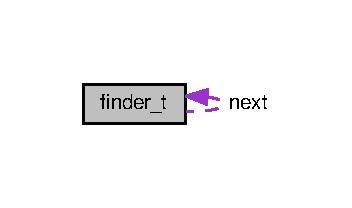
\includegraphics[width=188pt]{structfinder__t__coll__graph}
\end{center}
\end{figure}
\subsection*{Data Fields}
\begin{DoxyCompactItemize}
\item 
char $\ast$ \hyperlink{structfinder__t_aeac90097f29f7529968697163cea5c18}{filename}\hypertarget{structfinder__t_aeac90097f29f7529968697163cea5c18}{}\label{structfinder__t_aeac90097f29f7529968697163cea5c18}

\begin{DoxyCompactList}\small\item\em Found file name. \end{DoxyCompactList}\item 
struct \hyperlink{structfinder__t}{finder\+\_\+t} $\ast$ \hyperlink{structfinder__t_a7db9cac9324009990f14b7f84bf47d3c}{next}\hypertarget{structfinder__t_a7db9cac9324009990f14b7f84bf47d3c}{}\label{structfinder__t_a7db9cac9324009990f14b7f84bf47d3c}

\begin{DoxyCompactList}\small\item\em Next in the chain. \end{DoxyCompactList}\end{DoxyCompactItemize}


\subsection{Detailed Description}
A chained list of found file names. 

Definition at line 19 of file finder.\+h.



The documentation for this struct was generated from the following file\+:\begin{DoxyCompactItemize}
\item 
\hyperlink{finder_8h}{finder.\+h}\end{DoxyCompactItemize}

\hypertarget{structio__file__list}{}\section{io\+\_\+file\+\_\+list Struct Reference}
\label{structio__file__list}\index{io\+\_\+file\+\_\+list@{io\+\_\+file\+\_\+list}}
\subsection*{Data Fields}
\begin{DoxyCompactItemize}
\item 
char {\bfseries files} \mbox{[}I\+O\+\_\+\+D\+I\+R\+\_\+\+M\+A\+X\+\_\+\+F\+I\+L\+ES\mbox{]}\mbox{[}I\+O\+\_\+\+P\+A\+T\+H\+\_\+\+M\+A\+X\+\_\+\+S\+I\+ZE\mbox{]}\hypertarget{structio__file__list_aea2e7d487e7a0ce1737212bb7679dbcc}{}\label{structio__file__list_aea2e7d487e7a0ce1737212bb7679dbcc}

\item 
size\+\_\+t {\bfseries count}\hypertarget{structio__file__list_a76d971a3c552bc58ba9f0d5fceae9806}{}\label{structio__file__list_a76d971a3c552bc58ba9f0d5fceae9806}

\end{DoxyCompactItemize}


\subsection{Detailed Description}


Definition at line 17 of file io.\+h.



The documentation for this struct was generated from the following file\+:\begin{DoxyCompactItemize}
\item 
/home/claudio/git/smart-\/folder/src/io.\+h\end{DoxyCompactItemize}

\hypertarget{structparser__t}{}\section{parser\+\_\+t Struct Reference}
\label{structparser__t}\index{parser\+\_\+t@{parser\+\_\+t}}


Formal expression representation.  




{\ttfamily \#include $<$parser.\+h$>$}



Collaboration diagram for parser\+\_\+t\+:\nopagebreak
\begin{figure}[H]
\begin{center}
\leavevmode
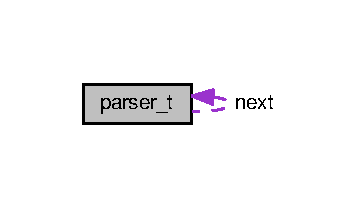
\includegraphics[width=172pt]{structparser__t__coll__graph}
\end{center}
\end{figure}
\subsection*{Data Fields}
\begin{DoxyCompactItemize}
\item 
\hyperlink{parser_8h_a4dcbe7148b91f50b0e7f3e08e780861d}{parser\+\_\+crit\+\_\+t} \hyperlink{structparser__t_af8e04406eee9097a92118be27b07eff7}{crit}
\begin{DoxyCompactList}\small\item\em The criteria for the token. \end{DoxyCompactList}\item 
void $\ast$ \hyperlink{structparser__t_a0f61d63b009d0880a89c843bd50d8d76}{value}
\begin{DoxyCompactList}\small\item\em The value of the criteria, the type depend on the type of \textquotesingle{}crit\textquotesingle{}. \end{DoxyCompactList}\item 
\hyperlink{parser_8h_ac721d0db2049edef01e62a2e63ff0472}{parser\+\_\+comp\+\_\+t} \hyperlink{structparser__t_a7bc05cec4ebb98215d11f1f354450f3d}{comp}
\begin{DoxyCompactList}\small\item\em The comparison to be used when evaluating the expression validity. \end{DoxyCompactList}\item 
struct \hyperlink{structparser__t}{parser\+\_\+t} $\ast$ \hyperlink{structparser__t_a044a5d882012dfdd9ea5e4f3a98fd8a2}{next}\hypertarget{structparser__t_a044a5d882012dfdd9ea5e4f3a98fd8a2}{}\label{structparser__t_a044a5d882012dfdd9ea5e4f3a98fd8a2}

\begin{DoxyCompactList}\small\item\em The next token in the expression. \end{DoxyCompactList}\end{DoxyCompactItemize}


\subsection{Detailed Description}
Formal expression representation. 

Contains the formal representation of the parsed expression in a ordered chained list. Each instance contains the information about a parsed expression token and the pointer to the {\ttfamily next} parsed expression token.

The order of the tokens in the chained list is not the same as the in the original string representation. Is has been reordered to encoded the priority of the operators and parenthesis in a infix notation 

Definition at line 71 of file parser.\+h.



\subsection{Field Documentation}
\index{parser\+\_\+t@{parser\+\_\+t}!comp@{comp}}
\index{comp@{comp}!parser\+\_\+t@{parser\+\_\+t}}
\subsubsection[{\texorpdfstring{comp}{comp}}]{\setlength{\rightskip}{0pt plus 5cm}{\bf parser\+\_\+comp\+\_\+t} comp}\hypertarget{structparser__t_a7bc05cec4ebb98215d11f1f354450f3d}{}\label{structparser__t_a7bc05cec4ebb98215d11f1f354450f3d}


The comparison to be used when evaluating the expression validity. 


\begin{DoxyItemize}
\item e.\+g. the {\ttfamily +} in the exp {\ttfamily -\/\+S\+I\+ZE +20}
\end{DoxyItemize}

\begin{DoxySeeAlso}{See also}
\hyperlink{parser_8h_ac721d0db2049edef01e62a2e63ff0472}{parser\+\_\+comp\+\_\+t} 
\end{DoxySeeAlso}


Definition at line 89 of file parser.\+h.

\index{parser\+\_\+t@{parser\+\_\+t}!crit@{crit}}
\index{crit@{crit}!parser\+\_\+t@{parser\+\_\+t}}
\subsubsection[{\texorpdfstring{crit}{crit}}]{\setlength{\rightskip}{0pt plus 5cm}{\bf parser\+\_\+crit\+\_\+t} crit}\hypertarget{structparser__t_af8e04406eee9097a92118be27b07eff7}{}\label{structparser__t_af8e04406eee9097a92118be27b07eff7}


The criteria for the token. 


\begin{DoxyItemize}
\item e.\+g. the {\ttfamily S\+I\+ZE} in the exp {\ttfamily -\/\+S\+I\+ZE +20}
\end{DoxyItemize}

\begin{DoxySeeAlso}{See also}
\hyperlink{parser_8h_a4dcbe7148b91f50b0e7f3e08e780861d}{parser\+\_\+crit\+\_\+t} 
\end{DoxySeeAlso}


Definition at line 77 of file parser.\+h.

\index{parser\+\_\+t@{parser\+\_\+t}!value@{value}}
\index{value@{value}!parser\+\_\+t@{parser\+\_\+t}}
\subsubsection[{\texorpdfstring{value}{value}}]{\setlength{\rightskip}{0pt plus 5cm}void$\ast$ value}\hypertarget{structparser__t_a0f61d63b009d0880a89c843bd50d8d76}{}\label{structparser__t_a0f61d63b009d0880a89c843bd50d8d76}


The value of the criteria, the type depend on the type of \textquotesingle{}crit\textquotesingle{}. 


\begin{DoxyItemize}
\item e.\+g. the {\ttfamily 20} in the exp {\ttfamily -\/\+S\+I\+ZE +20}
\end{DoxyItemize}

\begin{DoxySeeAlso}{See also}
\hyperlink{parser_8h_a4dcbe7148b91f50b0e7f3e08e780861d}{parser\+\_\+crit\+\_\+t} 
\end{DoxySeeAlso}


Definition at line 83 of file parser.\+h.



The documentation for this struct was generated from the following file\+:\begin{DoxyCompactItemize}
\item 
\hyperlink{parser_8h}{parser.\+h}\end{DoxyCompactItemize}

\hypertarget{structsearchfolder__t}{}\section{searchfolder\+\_\+t Struct Reference}
\label{structsearchfolder__t}\index{searchfolder\+\_\+t@{searchfolder\+\_\+t}}


Collaboration diagram for searchfolder\+\_\+t\+:\nopagebreak
\begin{figure}[H]
\begin{center}
\leavevmode
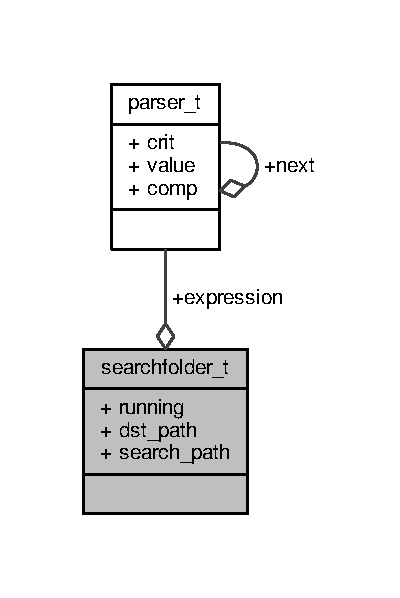
\includegraphics[width=185pt]{structsearchfolder__t__coll__graph}
\end{center}
\end{figure}
\subsection*{Data Fields}
\begin{DoxyCompactItemize}
\item 
bool {\bfseries running}\hypertarget{structsearchfolder__t_a36f7b6be7108281af77939ceaec42fd6}{}\label{structsearchfolder__t_a36f7b6be7108281af77939ceaec42fd6}

\item 
char $\ast$ {\bfseries dst\+\_\+path}\hypertarget{structsearchfolder__t_a74a7cec2bc63610109c58ef392d14e27}{}\label{structsearchfolder__t_a74a7cec2bc63610109c58ef392d14e27}

\item 
char $\ast$ {\bfseries search\+\_\+path}\hypertarget{structsearchfolder__t_a614ce96a64fa528698e05ce10070efe9}{}\label{structsearchfolder__t_a614ce96a64fa528698e05ce10070efe9}

\item 
\hyperlink{structparser__t}{parser\+\_\+t} $\ast$ {\bfseries expression}\hypertarget{structsearchfolder__t_a37eed245f4d8beb45412f8ba904643b2}{}\label{structsearchfolder__t_a37eed245f4d8beb45412f8ba904643b2}

\end{DoxyCompactItemize}


\subsection{Detailed Description}


Definition at line 11 of file searchfolder.\+c.



The documentation for this struct was generated from the following file\+:\begin{DoxyCompactItemize}
\item 
/home/claudio/git/smart-\/folder/src/searchfolder.\+c\end{DoxyCompactItemize}

\chapter{File Documentation}
\hypertarget{finder_8c}{}\section{finder.\+c File Reference}
\label{finder_8c}\index{finder.\+c@{finder.\+c}}


The finder retrives the list of files matching an expression.  


{\ttfamily \#include $<$dirent.\+h$>$}\\*
{\ttfamily \#include $<$string.\+h$>$}\\*
{\ttfamily \#include $<$sys/stat.\+h$>$}\\*
{\ttfamily \#include $<$unistd.\+h$>$}\\*
{\ttfamily \#include \char`\"{}finder.\+h\char`\"{}}\\*
{\ttfamily \#include \char`\"{}io.\+h\char`\"{}}\\*
{\ttfamily \#include \char`\"{}logger.\+h\char`\"{}}\\*
{\ttfamily \#include \char`\"{}vendor/uthash.\+h\char`\"{}}\\*
Include dependency graph for finder.\+c\+:\nopagebreak
\begin{figure}[H]
\begin{center}
\leavevmode
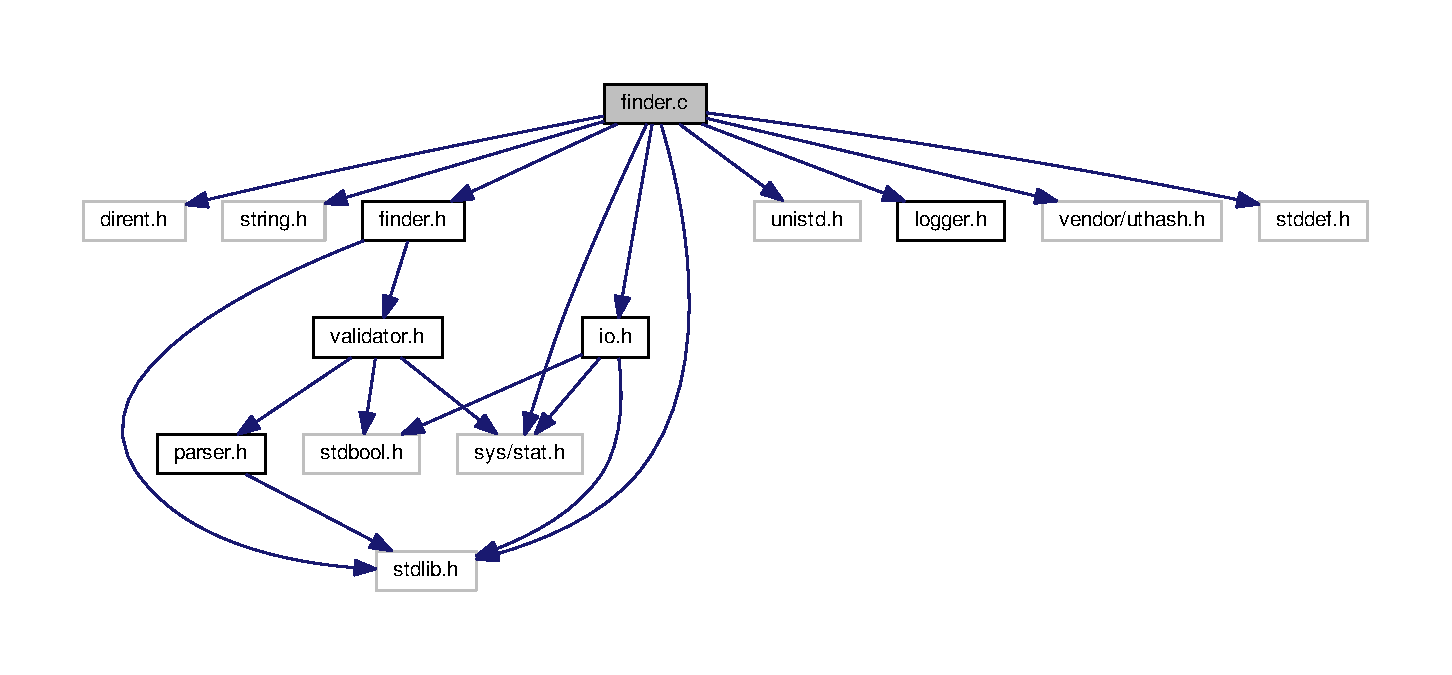
\includegraphics[width=350pt]{finder_8c__incl}
\end{center}
\end{figure}
\subsection*{Data Structures}
\begin{DoxyCompactItemize}
\item 
struct \hyperlink{structfile__t}{file\+\_\+t}
\begin{DoxyCompactList}\small\item\em Hashtable entry type used in {\ttfamily files}. \end{DoxyCompactList}\end{DoxyCompactItemize}
\subsection*{Typedefs}
\begin{DoxyCompactItemize}
\item 
typedef struct \hyperlink{structfile__t}{file\+\_\+t} \hyperlink{finder_8c_a67703743f2db513ba0def3664b12c985}{file\+\_\+t}
\begin{DoxyCompactList}\small\item\em Hashtable entry type used in {\ttfamily files}. \end{DoxyCompactList}\end{DoxyCompactItemize}
\subsection*{Functions}
\begin{DoxyCompactItemize}
\item 
static \hyperlink{structfinder__t}{finder\+\_\+t} $\ast$ \hyperlink{finder_8c_ac340644baae8a9317350f9e392c42368}{finder\+\_\+add\+\_\+found\+\_\+file} (char $\ast$filename, \hyperlink{structfinder__t}{finder\+\_\+t} $\ast$currentfile)
\begin{DoxyCompactList}\small\item\em Adds the found valid file to the list of found files. \end{DoxyCompactList}\item 
static bool \hyperlink{finder_8c_a025d083ddfaf8d1f24984a6f2dac247e}{finder\+\_\+hash\+\_\+exist} (long unsigned int inode)\hypertarget{finder_8c_a025d083ddfaf8d1f24984a6f2dac247e}{}\label{finder_8c_a025d083ddfaf8d1f24984a6f2dac247e}

\begin{DoxyCompactList}\small\item\em Verifies if an inode id has already been processed. \end{DoxyCompactList}\item 
static void \hyperlink{finder_8c_ab2145ca21a64cfad661093363718886d}{finder\+\_\+hash\+\_\+add} (long unsigned int inode)\hypertarget{finder_8c_ab2145ca21a64cfad661093363718886d}{}\label{finder_8c_ab2145ca21a64cfad661093363718886d}

\begin{DoxyCompactList}\small\item\em Adds an inode id to the hashtable of processed files. \end{DoxyCompactList}\item 
static void \hyperlink{finder_8c_aa6168ebbf59fa8aa0a5cb2ad29126119}{finder\+\_\+hash\+\_\+clear} ()\hypertarget{finder_8c_aa6168ebbf59fa8aa0a5cb2ad29126119}{}\label{finder_8c_aa6168ebbf59fa8aa0a5cb2ad29126119}

\begin{DoxyCompactList}\small\item\em Clears (frees) the processed files hashtable. \end{DoxyCompactList}\item 
static \hyperlink{structfinder__t}{finder\+\_\+t} $\ast$ \hyperlink{finder_8c_ac6a4585aa622dde1e020ec1315dc508c}{finder\+\_\+find\+\_\+in\+\_\+dir} (char $\ast$dir, \hyperlink{structfinder__t}{finder\+\_\+t} $\ast$filelist, \hyperlink{structparser__t}{parser\+\_\+t} $\ast$expression)
\begin{DoxyCompactList}\small\item\em Searches a directory recursively for files matching the expression. \end{DoxyCompactList}\item 
static \hyperlink{structfinder__t}{finder\+\_\+t} $\ast$ \hyperlink{finder_8c_a412e38578fba998523148c001076dd17}{finder\+\_\+process\+\_\+dent} (struct dirent $\ast$dent, char $\ast$dirpath, \hyperlink{structfinder__t}{finder\+\_\+t} $\ast$filelist, \hyperlink{structparser__t}{parser\+\_\+t} $\ast$expression)
\begin{DoxyCompactList}\small\item\em Processes a found directory entity. \end{DoxyCompactList}\item 
\hyperlink{structfinder__t}{finder\+\_\+t} $\ast$ \hyperlink{finder_8c_aed5e5c02d7edae974a768b4229453a97}{finder\+\_\+find} (char $\ast$search\+\_\+path, \hyperlink{structparser__t}{parser\+\_\+t} $\ast$expression)
\begin{DoxyCompactList}\small\item\em Finds the files in the {\ttfamily search\+\_\+path} matchin the {\ttfamily expression} \end{DoxyCompactList}\item 
void \hyperlink{finder_8c_a4a192d238e16272f38645ae201f1748f}{finder\+\_\+free} (\hyperlink{structfinder__t}{finder\+\_\+t} $\ast$finder)
\begin{DoxyCompactList}\small\item\em Frees the memory allocated by {\ttfamily finder} \end{DoxyCompactList}\end{DoxyCompactItemize}
\subsection*{Variables}
\begin{DoxyCompactItemize}
\item 
static struct \hyperlink{structfile__t}{file\+\_\+t} $\ast$ \hyperlink{finder_8c_a8bb2e2bcd7c9c20c6bdf286c0c1b67e4}{files} = N\+U\+LL
\begin{DoxyCompactList}\small\item\em Hashtable containing the processed files. \end{DoxyCompactList}\end{DoxyCompactItemize}


\subsection{Detailed Description}
The finder retrives the list of files matching an expression. 

A specified is search resursively for all find valid against a give filtering expression.

Symbolic links are followed, and an hashtable is kept with the id\textquotesingle{}s (inode id) of the processed paths to avoid processing the same paths twice and avoid infinte loops. 

\subsection{Typedef Documentation}
\index{finder.\+c@{finder.\+c}!file\+\_\+t@{file\+\_\+t}}
\index{file\+\_\+t@{file\+\_\+t}!finder.\+c@{finder.\+c}}
\subsubsection[{\texorpdfstring{file\+\_\+t}{file_t}}]{\setlength{\rightskip}{0pt plus 5cm}typedef struct {\bf file\+\_\+t}  {\bf file\+\_\+t}}\hypertarget{finder_8c_a67703743f2db513ba0def3664b12c985}{}\label{finder_8c_a67703743f2db513ba0def3664b12c985}


Hashtable entry type used in {\ttfamily files}. 

Each instance contains the inode id of a path already processed \begin{DoxySeeAlso}{See also}
\hyperlink{finder_8c_a8bb2e2bcd7c9c20c6bdf286c0c1b67e4}{files} 
\end{DoxySeeAlso}


\subsection{Function Documentation}
\index{finder.\+c@{finder.\+c}!finder\+\_\+add\+\_\+found\+\_\+file@{finder\+\_\+add\+\_\+found\+\_\+file}}
\index{finder\+\_\+add\+\_\+found\+\_\+file@{finder\+\_\+add\+\_\+found\+\_\+file}!finder.\+c@{finder.\+c}}
\subsubsection[{\texorpdfstring{finder\+\_\+add\+\_\+found\+\_\+file(char $\ast$filename, finder\+\_\+t $\ast$currentfile)}{finder_add_found_file(char *filename, finder_t *currentfile)}}]{\setlength{\rightskip}{0pt plus 5cm}static {\bf finder\+\_\+t}$\ast$ finder\+\_\+add\+\_\+found\+\_\+file (
\begin{DoxyParamCaption}
\item[{char $\ast$}]{filename, }
\item[{{\bf finder\+\_\+t} $\ast$}]{currentfile}
\end{DoxyParamCaption}
)\hspace{0.3cm}{\ttfamily [static]}}\hypertarget{finder_8c_ac340644baae8a9317350f9e392c42368}{}\label{finder_8c_ac340644baae8a9317350f9e392c42368}


Adds the found valid file to the list of found files. 


\begin{DoxyParams}{Parameters}
{\em filename} & Found file\textquotesingle{}s name \\
\hline
{\em currentfile} & Chained list of found files \\
\hline
\end{DoxyParams}
\begin{DoxyReturn}{Returns}
New pointer to the found files chained list 
\end{DoxyReturn}


Definition at line 41 of file finder.\+c.

\index{finder.\+c@{finder.\+c}!finder\+\_\+find@{finder\+\_\+find}}
\index{finder\+\_\+find@{finder\+\_\+find}!finder.\+c@{finder.\+c}}
\subsubsection[{\texorpdfstring{finder\+\_\+find(char $\ast$search\+\_\+path, parser\+\_\+t $\ast$expression)}{finder_find(char *search_path, parser_t *expression)}}]{\setlength{\rightskip}{0pt plus 5cm}{\bf finder\+\_\+t}$\ast$ finder\+\_\+find (
\begin{DoxyParamCaption}
\item[{char $\ast$}]{search\+\_\+path, }
\item[{{\bf parser\+\_\+t} $\ast$}]{expression}
\end{DoxyParamCaption}
)}\hypertarget{finder_8c_aed5e5c02d7edae974a768b4229453a97}{}\label{finder_8c_aed5e5c02d7edae974a768b4229453a97}


Finds the files in the {\ttfamily search\+\_\+path} matchin the {\ttfamily expression} 

Search is performed recusively and symbolic links are followed.


\begin{DoxyParams}{Parameters}
{\em search\+\_\+path} & Where to look for the files \\
\hline
{\em expression} & Filter expression used against found files \\
\hline
\end{DoxyParams}
\begin{DoxyReturn}{Returns}
List of found files 
\end{DoxyReturn}


Definition at line 172 of file finder.\+c.

\index{finder.\+c@{finder.\+c}!finder\+\_\+find\+\_\+in\+\_\+dir@{finder\+\_\+find\+\_\+in\+\_\+dir}}
\index{finder\+\_\+find\+\_\+in\+\_\+dir@{finder\+\_\+find\+\_\+in\+\_\+dir}!finder.\+c@{finder.\+c}}
\subsubsection[{\texorpdfstring{finder\+\_\+find\+\_\+in\+\_\+dir(char $\ast$dir, finder\+\_\+t $\ast$filelist, parser\+\_\+t $\ast$expression)}{finder_find_in_dir(char *dir, finder_t *filelist, parser_t *expression)}}]{\setlength{\rightskip}{0pt plus 5cm}static {\bf finder\+\_\+t} $\ast$ finder\+\_\+find\+\_\+in\+\_\+dir (
\begin{DoxyParamCaption}
\item[{char $\ast$}]{dir, }
\item[{{\bf finder\+\_\+t} $\ast$}]{filelist, }
\item[{{\bf parser\+\_\+t} $\ast$}]{expression}
\end{DoxyParamCaption}
)\hspace{0.3cm}{\ttfamily [static]}}\hypertarget{finder_8c_ac6a4585aa622dde1e020ec1315dc508c}{}\label{finder_8c_ac6a4585aa622dde1e020ec1315dc508c}


Searches a directory recursively for files matching the expression. 

Iterates over the directory entities and delegates their processing to {\ttfamily finder\+\_\+process\+\_\+dent}. Directories are added to the hastable of processed paths. 
\begin{DoxyParams}{Parameters}
{\em dir} & Directory full path \\
\hline
{\em filelist} & Pointer to the found files chained list \\
\hline
{\em expression} & Filtering expression \\
\hline
\end{DoxyParams}
\begin{DoxyReturn}{Returns}
New pointer to the found files chained list 
\end{DoxyReturn}


Definition at line 139 of file finder.\+c.

\index{finder.\+c@{finder.\+c}!finder\+\_\+free@{finder\+\_\+free}}
\index{finder\+\_\+free@{finder\+\_\+free}!finder.\+c@{finder.\+c}}
\subsubsection[{\texorpdfstring{finder\+\_\+free(finder\+\_\+t $\ast$finder)}{finder_free(finder_t *finder)}}]{\setlength{\rightskip}{0pt plus 5cm}void finder\+\_\+free (
\begin{DoxyParamCaption}
\item[{{\bf finder\+\_\+t} $\ast$}]{finder}
\end{DoxyParamCaption}
)}\hypertarget{finder_8c_a4a192d238e16272f38645ae201f1748f}{}\label{finder_8c_a4a192d238e16272f38645ae201f1748f}


Frees the memory allocated by {\ttfamily finder} 


\begin{DoxyParams}{Parameters}
{\em finder} & The instance to be freed \\
\hline
\end{DoxyParams}


Definition at line 179 of file finder.\+c.

\index{finder.\+c@{finder.\+c}!finder\+\_\+process\+\_\+dent@{finder\+\_\+process\+\_\+dent}}
\index{finder\+\_\+process\+\_\+dent@{finder\+\_\+process\+\_\+dent}!finder.\+c@{finder.\+c}}
\subsubsection[{\texorpdfstring{finder\+\_\+process\+\_\+dent(struct dirent $\ast$dent, char $\ast$dirpath, finder\+\_\+t $\ast$filelist, parser\+\_\+t $\ast$expression)}{finder_process_dent(struct dirent *dent, char *dirpath, finder_t *filelist, parser_t *expression)}}]{\setlength{\rightskip}{0pt plus 5cm}static {\bf finder\+\_\+t}$\ast$ finder\+\_\+process\+\_\+dent (
\begin{DoxyParamCaption}
\item[{struct dirent $\ast$}]{dent, }
\item[{char $\ast$}]{dirpath, }
\item[{{\bf finder\+\_\+t} $\ast$}]{filelist, }
\item[{{\bf parser\+\_\+t} $\ast$}]{expression}
\end{DoxyParamCaption}
)\hspace{0.3cm}{\ttfamily [static]}}\hypertarget{finder_8c_a412e38578fba998523148c001076dd17}{}\label{finder_8c_a412e38578fba998523148c001076dd17}


Processes a found directory entity. 

If it is a {\itshape directory}\+:
\begin{DoxyItemize}
\item we use {\ttfamily finder\+\_\+find\+\_\+in\+\_\+dir} to analyze the content
\end{DoxyItemize}

If it is a {\itshape regular file}\+:
\begin{DoxyItemize}
\item we check that if has not been processed yet
\item we check if is valid file against the expression
\item if the two previous conditions are met\+:
\begin{DoxyItemize}
\item it is added to the hashtable of processed files
\item it is added to the list of valid files found
\end{DoxyItemize}
\end{DoxyItemize}

If it is a {\itshape symbolic link}, we retrieve the target and check the target type\+:
\begin{DoxyItemize}
\item if it is a $\ast$directory, we proceed with the above conditions for directories
\item otherwise we proceed with above conditions for regular files
\end{DoxyItemize}


\begin{DoxyParams}{Parameters}
{\em dent} & Directory entity to process \\
\hline
{\em dirpath} & Directory entity full path \\
\hline
{\em filelist} & Pointer to the found files chained list \\
\hline
{\em expression} & Filtering expression \\
\hline
\end{DoxyParams}
\begin{DoxyReturn}{Returns}
New pointer to the found files chained list 
\end{DoxyReturn}


Definition at line 100 of file finder.\+c.



\subsection{Variable Documentation}
\index{finder.\+c@{finder.\+c}!files@{files}}
\index{files@{files}!finder.\+c@{finder.\+c}}
\subsubsection[{\texorpdfstring{files}{files}}]{\setlength{\rightskip}{0pt plus 5cm}struct {\bf file\+\_\+t}$\ast$ files = N\+U\+LL\hspace{0.3cm}{\ttfamily [static]}}\hypertarget{finder_8c_a8bb2e2bcd7c9c20c6bdf286c0c1b67e4}{}\label{finder_8c_a8bb2e2bcd7c9c20c6bdf286c0c1b67e4}


Hashtable containing the processed files. 

Used to avoid processing same paths twice. \begin{DoxySeeAlso}{See also}
\hyperlink{structfile__t}{file\+\_\+t} 
\end{DoxySeeAlso}


Definition at line 25 of file finder.\+c.


\hypertarget{finder_8h}{}\section{finder.\+h File Reference}
\label{finder_8h}\index{finder.\+h@{finder.\+h}}


The finder retrives the list of files matching an expression.  


{\ttfamily \#include $<$stdlib.\+h$>$}\\*
{\ttfamily \#include \char`\"{}validator.\+h\char`\"{}}\\*
Include dependency graph for finder.\+h\+:\nopagebreak
\begin{figure}[H]
\begin{center}
\leavevmode
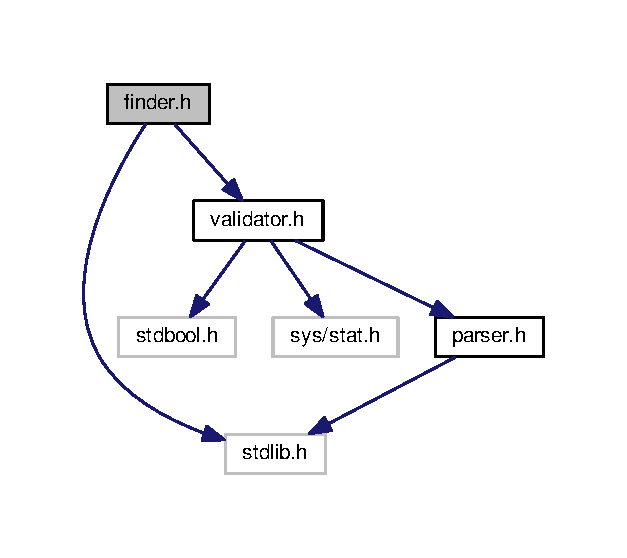
\includegraphics[width=301pt]{finder_8h__incl}
\end{center}
\end{figure}
This graph shows which files directly or indirectly include this file\+:\nopagebreak
\begin{figure}[H]
\begin{center}
\leavevmode
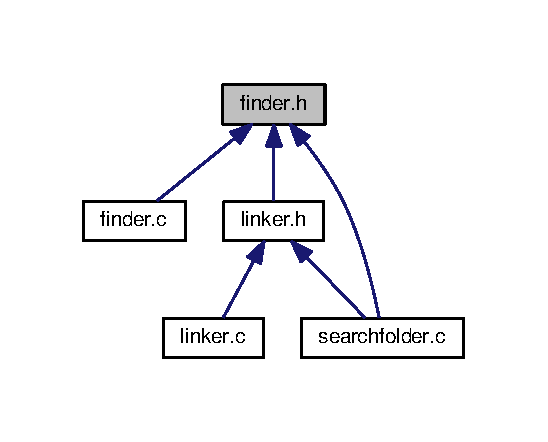
\includegraphics[width=263pt]{finder_8h__dep__incl}
\end{center}
\end{figure}
\subsection*{Data Structures}
\begin{DoxyCompactItemize}
\item 
struct \hyperlink{structfinder__t}{finder\+\_\+t}
\begin{DoxyCompactList}\small\item\em A chained list of found file names. \end{DoxyCompactList}\end{DoxyCompactItemize}
\subsection*{Typedefs}
\begin{DoxyCompactItemize}
\item 
typedef struct \hyperlink{structfinder__t}{finder\+\_\+t} \hyperlink{finder_8h_a0a83931979ff8debdb25fb5b4c486af9}{finder\+\_\+t}\hypertarget{finder_8h_a0a83931979ff8debdb25fb5b4c486af9}{}\label{finder_8h_a0a83931979ff8debdb25fb5b4c486af9}

\begin{DoxyCompactList}\small\item\em A chained list of found file names. \end{DoxyCompactList}\end{DoxyCompactItemize}
\subsection*{Functions}
\begin{DoxyCompactItemize}
\item 
\hyperlink{structfinder__t}{finder\+\_\+t} $\ast$ \hyperlink{finder_8h_aed5e5c02d7edae974a768b4229453a97}{finder\+\_\+find} (char $\ast$search\+\_\+path, \hyperlink{structparser__t}{parser\+\_\+t} $\ast$expression)
\begin{DoxyCompactList}\small\item\em Finds the files in the {\ttfamily search\+\_\+path} matchin the {\ttfamily expression} \end{DoxyCompactList}\item 
void \hyperlink{finder_8h_a4a192d238e16272f38645ae201f1748f}{finder\+\_\+free} (\hyperlink{structfinder__t}{finder\+\_\+t} $\ast$finder)
\begin{DoxyCompactList}\small\item\em Frees the memory allocated by {\ttfamily finder} \end{DoxyCompactList}\end{DoxyCompactItemize}


\subsection{Detailed Description}
The finder retrives the list of files matching an expression. 

A specified is search resursively for all find valid against a give filtering expression.

Symbolic links are followed, and an hashtable is kept with the id\textquotesingle{}s (inode id) of the found files to avoid processing the same paths twice and avoid infinte loops. 

\subsection{Function Documentation}
\index{finder.\+h@{finder.\+h}!finder\+\_\+find@{finder\+\_\+find}}
\index{finder\+\_\+find@{finder\+\_\+find}!finder.\+h@{finder.\+h}}
\subsubsection[{\texorpdfstring{finder\+\_\+find(char $\ast$search\+\_\+path, parser\+\_\+t $\ast$expression)}{finder_find(char *search_path, parser_t *expression)}}]{\setlength{\rightskip}{0pt plus 5cm}{\bf finder\+\_\+t}$\ast$ finder\+\_\+find (
\begin{DoxyParamCaption}
\item[{char $\ast$}]{search\+\_\+path, }
\item[{{\bf parser\+\_\+t} $\ast$}]{expression}
\end{DoxyParamCaption}
)}\hypertarget{finder_8h_aed5e5c02d7edae974a768b4229453a97}{}\label{finder_8h_aed5e5c02d7edae974a768b4229453a97}


Finds the files in the {\ttfamily search\+\_\+path} matchin the {\ttfamily expression} 

Search is performed recusively and symbolic links are followed.


\begin{DoxyParams}{Parameters}
{\em search\+\_\+path} & Where to look for the files \\
\hline
{\em expression} & Filter expression used against found files \\
\hline
\end{DoxyParams}
\begin{DoxyReturn}{Returns}
List of found files 
\end{DoxyReturn}


Definition at line 172 of file finder.\+c.

\index{finder.\+h@{finder.\+h}!finder\+\_\+free@{finder\+\_\+free}}
\index{finder\+\_\+free@{finder\+\_\+free}!finder.\+h@{finder.\+h}}
\subsubsection[{\texorpdfstring{finder\+\_\+free(finder\+\_\+t $\ast$finder)}{finder_free(finder_t *finder)}}]{\setlength{\rightskip}{0pt plus 5cm}void finder\+\_\+free (
\begin{DoxyParamCaption}
\item[{{\bf finder\+\_\+t} $\ast$}]{finder}
\end{DoxyParamCaption}
)}\hypertarget{finder_8h_a4a192d238e16272f38645ae201f1748f}{}\label{finder_8h_a4a192d238e16272f38645ae201f1748f}


Frees the memory allocated by {\ttfamily finder} 


\begin{DoxyParams}{Parameters}
{\em finder} & The instance to be freed \\
\hline
\end{DoxyParams}


Definition at line 179 of file finder.\+c.


\hypertarget{io_8c}{}\section{io.\+c File Reference}
\label{io_8c}\index{io.\+c@{io.\+c}}


Helpers function around system calls for IO purpose.  


{\ttfamily \#include $<$stdio.\+h$>$}\\*
{\ttfamily \#include $<$stdlib.\+h$>$}\\*
{\ttfamily \#include $<$string.\+h$>$}\\*
{\ttfamily \#include $<$unistd.\+h$>$}\\*
{\ttfamily \#include $<$fcntl.\+h$>$}\\*
{\ttfamily \#include $<$dirent.\+h$>$}\\*
{\ttfamily \#include \char`\"{}io.\+h\char`\"{}}\\*
{\ttfamily \#include \char`\"{}logger.\+h\char`\"{}}\\*
Include dependency graph for io.\+c\+:\nopagebreak
\begin{figure}[H]
\begin{center}
\leavevmode
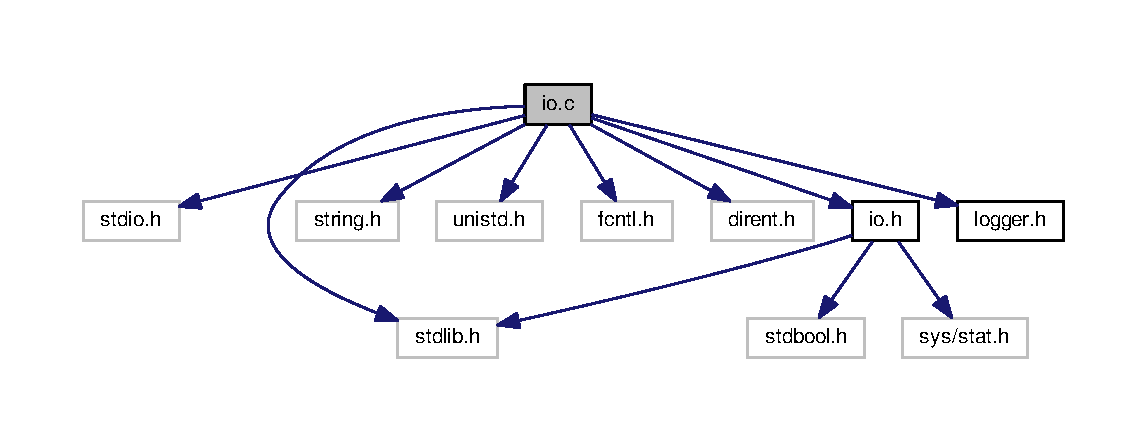
\includegraphics[width=350pt]{io_8c__incl}
\end{center}
\end{figure}
\subsection*{Macros}
\begin{DoxyCompactItemize}
\item 
\#define {\bfseries I\+O\+\_\+\+T\+M\+P\+\_\+\+B\+U\+F\+\_\+\+S\+I\+ZE}~4096\hypertarget{io_8c_adfab913360aa0f08f7a5f5bc02596913}{}\label{io_8c_adfab913360aa0f08f7a5f5bc02596913}

\item 
\#define {\bfseries I\+O\+\_\+\+D\+E\+F\+A\+U\+L\+T\+\_\+\+P\+E\+RM}~0644\hypertarget{io_8c_af0da451625569400b3945b0c4b659e8a}{}\label{io_8c_af0da451625569400b3945b0c4b659e8a}

\item 
\#define {\bfseries I\+O\+\_\+\+D\+E\+F\+A\+U\+L\+T\+\_\+\+M\+O\+DE}~S\+\_\+\+I\+R\+W\+XU $\vert$ S\+\_\+\+I\+R\+W\+XG\hypertarget{io_8c_a6f438420fd5a13d4bb608b397ca56db9}{}\label{io_8c_a6f438420fd5a13d4bb608b397ca56db9}

\end{DoxyCompactItemize}
\subsection*{Functions}
\begin{DoxyCompactItemize}
\item 
bool \hyperlink{io_8c_a159fbc793fca80d55a1f441af6c0fff6}{io\+\_\+file\+\_\+exists} (char $\ast$path)
\begin{DoxyCompactList}\small\item\em Determine if a file in the specified path exists. \end{DoxyCompactList}\item 
int \hyperlink{io_8c_a9954a448697a3890f6de7e204c0bbc63}{io\+\_\+file\+\_\+read\+\_\+content} (char $\ast$path, char $\ast$dst\+\_\+buffer, size\+\_\+t buf\+\_\+size)
\begin{DoxyCompactList}\small\item\em Fully read a file and put it in the destination buffer. \end{DoxyCompactList}\item 
int \hyperlink{io_8c_aa7db87fd66e6470dc35ce6683302c27a}{io\+\_\+file\+\_\+write} (char $\ast$path, char $\ast$content)
\begin{DoxyCompactList}\small\item\em Write the content in the specified path. \end{DoxyCompactList}\item 
int \hyperlink{io_8c_a0f360b2e15078bfa6c1870168c7c5290}{io\+\_\+file\+\_\+write\+\_\+fd} (int fd, char $\ast$content)
\begin{DoxyCompactList}\small\item\em Write the content in the specified path. \end{DoxyCompactList}\item 
int \hyperlink{io_8c_af87219af18ad7932389bf1f6074b490e}{io\+\_\+file\+\_\+delete} (char $\ast$path)
\begin{DoxyCompactList}\small\item\em Delete a file. \end{DoxyCompactList}\item 
bool \hyperlink{io_8c_a923afb970c89a949e354ca2e37e2b41a}{io\+\_\+directory\+\_\+exists} (char $\ast$path)
\begin{DoxyCompactList}\small\item\em Determine if a directory in the specified path exists. \end{DoxyCompactList}\item 
\hyperlink{structio__file__list}{io\+\_\+file\+\_\+list} $\ast$ \hyperlink{io_8c_adb8d68b54b043f5118a4cbfd49a8ec51}{io\+\_\+directory\+\_\+get\+\_\+all} (char $\ast$path)
\begin{DoxyCompactList}\small\item\em Get all element contained in the specified directory. \end{DoxyCompactList}\item 
void \hyperlink{io_8c_a0a8c4afe4b5ca881249bd543d0e10893}{io\+\_\+directory\+\_\+get\+\_\+all\+\_\+free} (\hyperlink{structio__file__list}{io\+\_\+file\+\_\+list} $\ast$filelist)
\begin{DoxyCompactList}\small\item\em Free a previously created list of files. \end{DoxyCompactList}\item 
int \hyperlink{io_8c_a8ba974718b179b7e353ca509d9624025}{io\+\_\+directory\+\_\+create} (char $\ast$path)
\begin{DoxyCompactList}\small\item\em Create a directory in the specified path. \end{DoxyCompactList}\item 
int \hyperlink{io_8c_aaa99d4fcb2d73da0b4f999576139cbdf}{io\+\_\+directory\+\_\+create\+\_\+parent} (char $\ast$path)
\begin{DoxyCompactList}\small\item\em Create a directory in the specified path and all its parents. \end{DoxyCompactList}\item 
int \hyperlink{io_8c_a6624d60efc4bbe979fcaf6f1ff7706a1}{io\+\_\+directory\+\_\+delete} (char $\ast$path)
\begin{DoxyCompactList}\small\item\em Delete a directory and all childrens. \end{DoxyCompactList}\item 
bool \hyperlink{io_8c_aaec48033f093fde5912023e4dc887121}{io\+\_\+link\+\_\+exists} (char $\ast$path)
\begin{DoxyCompactList}\small\item\em Determine if a link in the specified path exists. \end{DoxyCompactList}\end{DoxyCompactItemize}


\subsection{Detailed Description}
Helpers function around system calls for IO purpose. 

\begin{DoxyAuthor}{Author}
Claudio Sousa, Gonzalez David 
\end{DoxyAuthor}


\subsection{Function Documentation}
\index{io.\+c@{io.\+c}!io\+\_\+directory\+\_\+create@{io\+\_\+directory\+\_\+create}}
\index{io\+\_\+directory\+\_\+create@{io\+\_\+directory\+\_\+create}!io.\+c@{io.\+c}}
\subsubsection[{\texorpdfstring{io\+\_\+directory\+\_\+create(char $\ast$path)}{io_directory_create(char *path)}}]{\setlength{\rightskip}{0pt plus 5cm}int io\+\_\+directory\+\_\+create (
\begin{DoxyParamCaption}
\item[{char $\ast$}]{path}
\end{DoxyParamCaption}
)}\hypertarget{io_8c_a8ba974718b179b7e353ca509d9624025}{}\label{io_8c_a8ba974718b179b7e353ca509d9624025}


Create a directory in the specified path. 


\begin{DoxyParams}{Parameters}
{\em path} & Dir path to create \\
\hline
\end{DoxyParams}
\begin{DoxyReturn}{Returns}
0 if created, 1 if error 
\end{DoxyReturn}


Definition at line 124 of file io.\+c.

\index{io.\+c@{io.\+c}!io\+\_\+directory\+\_\+create\+\_\+parent@{io\+\_\+directory\+\_\+create\+\_\+parent}}
\index{io\+\_\+directory\+\_\+create\+\_\+parent@{io\+\_\+directory\+\_\+create\+\_\+parent}!io.\+c@{io.\+c}}
\subsubsection[{\texorpdfstring{io\+\_\+directory\+\_\+create\+\_\+parent(char $\ast$path)}{io_directory_create_parent(char *path)}}]{\setlength{\rightskip}{0pt plus 5cm}int io\+\_\+directory\+\_\+create\+\_\+parent (
\begin{DoxyParamCaption}
\item[{char $\ast$}]{path}
\end{DoxyParamCaption}
)}\hypertarget{io_8c_aaa99d4fcb2d73da0b4f999576139cbdf}{}\label{io_8c_aaa99d4fcb2d73da0b4f999576139cbdf}


Create a directory in the specified path and all its parents. 

If a the directory and its parents already exist, nothing is done. 
\begin{DoxyParams}{Parameters}
{\em path} & Dir path to create \\
\hline
\end{DoxyParams}
\begin{DoxyReturn}{Returns}
0 if created, 1 if error 
\end{DoxyReturn}


Definition at line 133 of file io.\+c.

\index{io.\+c@{io.\+c}!io\+\_\+directory\+\_\+delete@{io\+\_\+directory\+\_\+delete}}
\index{io\+\_\+directory\+\_\+delete@{io\+\_\+directory\+\_\+delete}!io.\+c@{io.\+c}}
\subsubsection[{\texorpdfstring{io\+\_\+directory\+\_\+delete(char $\ast$path)}{io_directory_delete(char *path)}}]{\setlength{\rightskip}{0pt plus 5cm}int io\+\_\+directory\+\_\+delete (
\begin{DoxyParamCaption}
\item[{char $\ast$}]{path}
\end{DoxyParamCaption}
)}\hypertarget{io_8c_a6624d60efc4bbe979fcaf6f1ff7706a1}{}\label{io_8c_a6624d60efc4bbe979fcaf6f1ff7706a1}


Delete a directory and all childrens. 


\begin{DoxyParams}{Parameters}
{\em path} & Directory path to delete \\
\hline
\end{DoxyParams}
\begin{DoxyReturn}{Returns}
0 if deleted, 1 if error 
\end{DoxyReturn}


Definition at line 152 of file io.\+c.

\index{io.\+c@{io.\+c}!io\+\_\+directory\+\_\+exists@{io\+\_\+directory\+\_\+exists}}
\index{io\+\_\+directory\+\_\+exists@{io\+\_\+directory\+\_\+exists}!io.\+c@{io.\+c}}
\subsubsection[{\texorpdfstring{io\+\_\+directory\+\_\+exists(char $\ast$path)}{io_directory_exists(char *path)}}]{\setlength{\rightskip}{0pt plus 5cm}bool io\+\_\+directory\+\_\+exists (
\begin{DoxyParamCaption}
\item[{char $\ast$}]{path}
\end{DoxyParamCaption}
)}\hypertarget{io_8c_a923afb970c89a949e354ca2e37e2b41a}{}\label{io_8c_a923afb970c89a949e354ca2e37e2b41a}


Determine if a directory in the specified path exists. 


\begin{DoxyParams}{Parameters}
{\em path} & File path to check \\
\hline
\end{DoxyParams}
\begin{DoxyReturn}{Returns}
True if exists, false otherwise 
\end{DoxyReturn}


Definition at line 82 of file io.\+c.

\index{io.\+c@{io.\+c}!io\+\_\+directory\+\_\+get\+\_\+all@{io\+\_\+directory\+\_\+get\+\_\+all}}
\index{io\+\_\+directory\+\_\+get\+\_\+all@{io\+\_\+directory\+\_\+get\+\_\+all}!io.\+c@{io.\+c}}
\subsubsection[{\texorpdfstring{io\+\_\+directory\+\_\+get\+\_\+all(char $\ast$path)}{io_directory_get_all(char *path)}}]{\setlength{\rightskip}{0pt plus 5cm}{\bf io\+\_\+file\+\_\+list}$\ast$ io\+\_\+directory\+\_\+get\+\_\+all (
\begin{DoxyParamCaption}
\item[{char $\ast$}]{path}
\end{DoxyParamCaption}
)}\hypertarget{io_8c_adb8d68b54b043f5118a4cbfd49a8ec51}{}\label{io_8c_adb8d68b54b043f5118a4cbfd49a8ec51}


Get all element contained in the specified directory. 


\begin{DoxyParams}{Parameters}
{\em path} & Dir path to scan \\
\hline
\end{DoxyParams}
\begin{DoxyReturn}{Returns}
List of files 
\end{DoxyReturn}


Definition at line 87 of file io.\+c.

\index{io.\+c@{io.\+c}!io\+\_\+directory\+\_\+get\+\_\+all\+\_\+free@{io\+\_\+directory\+\_\+get\+\_\+all\+\_\+free}}
\index{io\+\_\+directory\+\_\+get\+\_\+all\+\_\+free@{io\+\_\+directory\+\_\+get\+\_\+all\+\_\+free}!io.\+c@{io.\+c}}
\subsubsection[{\texorpdfstring{io\+\_\+directory\+\_\+get\+\_\+all\+\_\+free(io\+\_\+file\+\_\+list $\ast$filelist)}{io_directory_get_all_free(io_file_list *filelist)}}]{\setlength{\rightskip}{0pt plus 5cm}void io\+\_\+directory\+\_\+get\+\_\+all\+\_\+free (
\begin{DoxyParamCaption}
\item[{{\bf io\+\_\+file\+\_\+list} $\ast$}]{filelist}
\end{DoxyParamCaption}
)}\hypertarget{io_8c_a0a8c4afe4b5ca881249bd543d0e10893}{}\label{io_8c_a0a8c4afe4b5ca881249bd543d0e10893}


Free a previously created list of files. 


\begin{DoxyParams}{Parameters}
{\em filelist} & File list to free \\
\hline
\end{DoxyParams}


Definition at line 120 of file io.\+c.

\index{io.\+c@{io.\+c}!io\+\_\+file\+\_\+delete@{io\+\_\+file\+\_\+delete}}
\index{io\+\_\+file\+\_\+delete@{io\+\_\+file\+\_\+delete}!io.\+c@{io.\+c}}
\subsubsection[{\texorpdfstring{io\+\_\+file\+\_\+delete(char $\ast$path)}{io_file_delete(char *path)}}]{\setlength{\rightskip}{0pt plus 5cm}int io\+\_\+file\+\_\+delete (
\begin{DoxyParamCaption}
\item[{char $\ast$}]{path}
\end{DoxyParamCaption}
)}\hypertarget{io_8c_af87219af18ad7932389bf1f6074b490e}{}\label{io_8c_af87219af18ad7932389bf1f6074b490e}


Delete a file. 


\begin{DoxyParams}{Parameters}
{\em path} & File path to delete \\
\hline
\end{DoxyParams}
\begin{DoxyReturn}{Returns}
0 if deleted, 1 if error 
\end{DoxyReturn}


Definition at line 73 of file io.\+c.

\index{io.\+c@{io.\+c}!io\+\_\+file\+\_\+exists@{io\+\_\+file\+\_\+exists}}
\index{io\+\_\+file\+\_\+exists@{io\+\_\+file\+\_\+exists}!io.\+c@{io.\+c}}
\subsubsection[{\texorpdfstring{io\+\_\+file\+\_\+exists(char $\ast$path)}{io_file_exists(char *path)}}]{\setlength{\rightskip}{0pt plus 5cm}bool io\+\_\+file\+\_\+exists (
\begin{DoxyParamCaption}
\item[{char $\ast$}]{path}
\end{DoxyParamCaption}
)}\hypertarget{io_8c_a159fbc793fca80d55a1f441af6c0fff6}{}\label{io_8c_a159fbc793fca80d55a1f441af6c0fff6}


Determine if a file in the specified path exists. 


\begin{DoxyParams}{Parameters}
{\em path} & File path to check \\
\hline
\end{DoxyParams}
\begin{DoxyReturn}{Returns}
True if exists, false otherwise 
\end{DoxyReturn}


Definition at line 20 of file io.\+c.

\index{io.\+c@{io.\+c}!io\+\_\+file\+\_\+read\+\_\+content@{io\+\_\+file\+\_\+read\+\_\+content}}
\index{io\+\_\+file\+\_\+read\+\_\+content@{io\+\_\+file\+\_\+read\+\_\+content}!io.\+c@{io.\+c}}
\subsubsection[{\texorpdfstring{io\+\_\+file\+\_\+read\+\_\+content(char $\ast$path, char $\ast$dst\+\_\+buffer, size\+\_\+t buf\+\_\+size)}{io_file_read_content(char *path, char *dst_buffer, size_t buf_size)}}]{\setlength{\rightskip}{0pt plus 5cm}int io\+\_\+file\+\_\+read\+\_\+content (
\begin{DoxyParamCaption}
\item[{char $\ast$}]{path, }
\item[{char $\ast$}]{dst\+\_\+buffer, }
\item[{size\+\_\+t}]{buf\+\_\+size}
\end{DoxyParamCaption}
)}\hypertarget{io_8c_a9954a448697a3890f6de7e204c0bbc63}{}\label{io_8c_a9954a448697a3890f6de7e204c0bbc63}


Fully read a file and put it in the destination buffer. 


\begin{DoxyParams}{Parameters}
{\em path} & File path to read \\
\hline
{\em dst\+\_\+buffer} & Buffer to put the result \\
\hline
\end{DoxyParams}
\begin{DoxyReturn}{Returns}
Success result, return 0 only when it has fully read it, 1 if any error occurs 
\end{DoxyReturn}


Definition at line 25 of file io.\+c.

\index{io.\+c@{io.\+c}!io\+\_\+file\+\_\+write@{io\+\_\+file\+\_\+write}}
\index{io\+\_\+file\+\_\+write@{io\+\_\+file\+\_\+write}!io.\+c@{io.\+c}}
\subsubsection[{\texorpdfstring{io\+\_\+file\+\_\+write(char $\ast$path, char $\ast$content)}{io_file_write(char *path, char *content)}}]{\setlength{\rightskip}{0pt plus 5cm}int io\+\_\+file\+\_\+write (
\begin{DoxyParamCaption}
\item[{char $\ast$}]{path, }
\item[{char $\ast$}]{content}
\end{DoxyParamCaption}
)}\hypertarget{io_8c_aa7db87fd66e6470dc35ce6683302c27a}{}\label{io_8c_aa7db87fd66e6470dc35ce6683302c27a}


Write the content in the specified path. 


\begin{DoxyParams}{Parameters}
{\em path} & File path to write in \\
\hline
{\em content} & Content to put in the file \\
\hline
\end{DoxyParams}
\begin{DoxyReturn}{Returns}
Success result, return 0 only when it has fully written it, 1 if any error occurs 
\end{DoxyReturn}


Definition at line 45 of file io.\+c.

\index{io.\+c@{io.\+c}!io\+\_\+file\+\_\+write\+\_\+fd@{io\+\_\+file\+\_\+write\+\_\+fd}}
\index{io\+\_\+file\+\_\+write\+\_\+fd@{io\+\_\+file\+\_\+write\+\_\+fd}!io.\+c@{io.\+c}}
\subsubsection[{\texorpdfstring{io\+\_\+file\+\_\+write\+\_\+fd(int fd, char $\ast$content)}{io_file_write_fd(int fd, char *content)}}]{\setlength{\rightskip}{0pt plus 5cm}int io\+\_\+file\+\_\+write\+\_\+fd (
\begin{DoxyParamCaption}
\item[{int}]{fd, }
\item[{char $\ast$}]{content}
\end{DoxyParamCaption}
)}\hypertarget{io_8c_a0f360b2e15078bfa6c1870168c7c5290}{}\label{io_8c_a0f360b2e15078bfa6c1870168c7c5290}


Write the content in the specified path. 


\begin{DoxyParams}{Parameters}
{\em fd} & file descriptor to write in \\
\hline
{\em content} & Content to put in the file descriptor \\
\hline
\end{DoxyParams}
\begin{DoxyReturn}{Returns}
Success result, return 0 only when it has fully written it, 1 if any error occurs 
\end{DoxyReturn}


Definition at line 61 of file io.\+c.

\index{io.\+c@{io.\+c}!io\+\_\+link\+\_\+exists@{io\+\_\+link\+\_\+exists}}
\index{io\+\_\+link\+\_\+exists@{io\+\_\+link\+\_\+exists}!io.\+c@{io.\+c}}
\subsubsection[{\texorpdfstring{io\+\_\+link\+\_\+exists(char $\ast$path)}{io_link_exists(char *path)}}]{\setlength{\rightskip}{0pt plus 5cm}bool io\+\_\+link\+\_\+exists (
\begin{DoxyParamCaption}
\item[{char $\ast$}]{path}
\end{DoxyParamCaption}
)}\hypertarget{io_8c_aaec48033f093fde5912023e4dc887121}{}\label{io_8c_aaec48033f093fde5912023e4dc887121}


Determine if a link in the specified path exists. 


\begin{DoxyParams}{Parameters}
{\em path} & Link path to check \\
\hline
\end{DoxyParams}
\begin{DoxyReturn}{Returns}
True if exists, false otherwise 
\end{DoxyReturn}


Definition at line 169 of file io.\+c.


\hypertarget{io_8h}{}\section{io.\+h File Reference}
\label{io_8h}\index{io.\+h@{io.\+h}}


Helpers function around system calls for IO purpose.  


{\ttfamily \#include $<$stdlib.\+h$>$}\\*
{\ttfamily \#include $<$stdbool.\+h$>$}\\*
{\ttfamily \#include $<$sys/stat.\+h$>$}\\*
Include dependency graph for io.\+h\+:\nopagebreak
\begin{figure}[H]
\begin{center}
\leavevmode
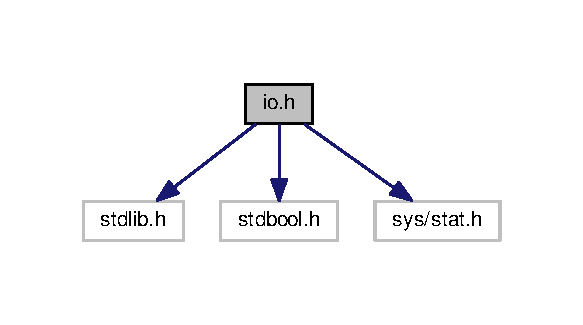
\includegraphics[width=280pt]{io_8h__incl}
\end{center}
\end{figure}
This graph shows which files directly or indirectly include this file\+:
\nopagebreak
\begin{figure}[H]
\begin{center}
\leavevmode
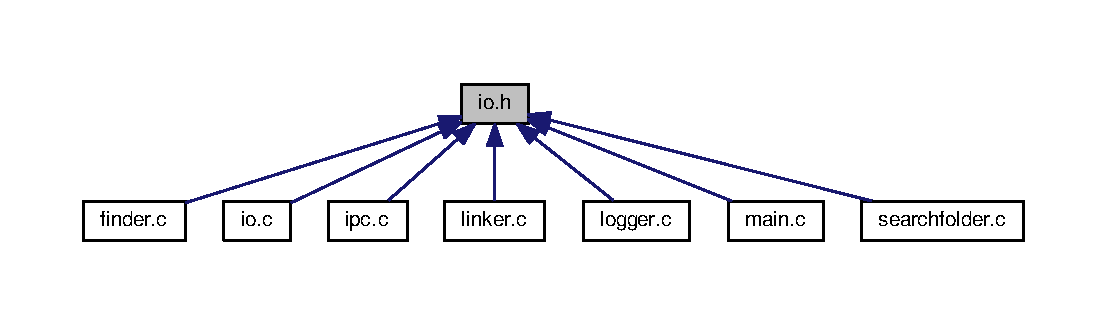
\includegraphics[width=350pt]{io_8h__dep__incl}
\end{center}
\end{figure}
\subsection*{Data Structures}
\begin{DoxyCompactItemize}
\item 
struct \hyperlink{structio__file__list}{io\+\_\+file\+\_\+list}
\begin{DoxyCompactList}\small\item\em Container for file lists (fixed size for simplification), used by \hyperlink{io_8c_adb8d68b54b043f5118a4cbfd49a8ec51}{io\+\_\+directory\+\_\+get\+\_\+all()}. \end{DoxyCompactList}\end{DoxyCompactItemize}
\subsection*{Macros}
\begin{DoxyCompactItemize}
\item 
\#define \hyperlink{io_8h_a3459a8a15f99dc120380d828bc7a4cd8}{I\+O\+\_\+\+P\+A\+T\+H\+\_\+\+M\+A\+X\+\_\+\+S\+I\+ZE}~4096\hypertarget{io_8h_a3459a8a15f99dc120380d828bc7a4cd8}{}\label{io_8h_a3459a8a15f99dc120380d828bc7a4cd8}

\begin{DoxyCompactList}\small\item\em Maximum string size for path. \end{DoxyCompactList}\item 
\#define \hyperlink{io_8h_a4f83737c59830cd64451f3e29bfe714d}{I\+O\+\_\+\+P\+A\+T\+H\+\_\+\+S\+EP}~\textquotesingle{}/\textquotesingle{}\hypertarget{io_8h_a4f83737c59830cd64451f3e29bfe714d}{}\label{io_8h_a4f83737c59830cd64451f3e29bfe714d}

\begin{DoxyCompactList}\small\item\em Path separator for path construction. \end{DoxyCompactList}\item 
\#define \hyperlink{io_8h_a467d28fd66a94e856cb73b80110d730a}{I\+O\+\_\+\+D\+I\+R\+\_\+\+M\+A\+X\+\_\+\+F\+I\+L\+ES}~1024\hypertarget{io_8h_a467d28fd66a94e856cb73b80110d730a}{}\label{io_8h_a467d28fd66a94e856cb73b80110d730a}

\begin{DoxyCompactList}\small\item\em Maximum files allowed in the list of files. \end{DoxyCompactList}\end{DoxyCompactItemize}
\subsection*{Typedefs}
\begin{DoxyCompactItemize}
\item 
typedef struct \hyperlink{structio__file__list}{io\+\_\+file\+\_\+list} \hyperlink{io_8h_aff2e2b3b9ce6a73d29d9a69f32a4c8ee}{io\+\_\+file\+\_\+list}\hypertarget{io_8h_aff2e2b3b9ce6a73d29d9a69f32a4c8ee}{}\label{io_8h_aff2e2b3b9ce6a73d29d9a69f32a4c8ee}

\begin{DoxyCompactList}\small\item\em Container for file lists (fixed size for simplification), used by \hyperlink{io_8c_adb8d68b54b043f5118a4cbfd49a8ec51}{io\+\_\+directory\+\_\+get\+\_\+all()}. \end{DoxyCompactList}\end{DoxyCompactItemize}
\subsection*{Functions}
\begin{DoxyCompactItemize}
\item 
bool \hyperlink{io_8h_a159fbc793fca80d55a1f441af6c0fff6}{io\+\_\+file\+\_\+exists} (char $\ast$path)
\begin{DoxyCompactList}\small\item\em Determine if a file in the specified path exists. \end{DoxyCompactList}\item 
int \hyperlink{io_8h_a9954a448697a3890f6de7e204c0bbc63}{io\+\_\+file\+\_\+read\+\_\+content} (char $\ast$path, char $\ast$dst\+\_\+buffer, size\+\_\+t buf\+\_\+size)
\begin{DoxyCompactList}\small\item\em Fully read a file and put it in the destination buffer. \end{DoxyCompactList}\item 
int \hyperlink{io_8h_aa7db87fd66e6470dc35ce6683302c27a}{io\+\_\+file\+\_\+write} (char $\ast$path, char $\ast$content)
\begin{DoxyCompactList}\small\item\em Write the content in the specified path. \end{DoxyCompactList}\item 
int \hyperlink{io_8h_a0f360b2e15078bfa6c1870168c7c5290}{io\+\_\+file\+\_\+write\+\_\+fd} (int fd, char $\ast$content)
\begin{DoxyCompactList}\small\item\em Write the content in the specified path. \end{DoxyCompactList}\item 
int \hyperlink{io_8h_af87219af18ad7932389bf1f6074b490e}{io\+\_\+file\+\_\+delete} (char $\ast$path)
\begin{DoxyCompactList}\small\item\em Delete a file. \end{DoxyCompactList}\item 
bool \hyperlink{io_8h_a923afb970c89a949e354ca2e37e2b41a}{io\+\_\+directory\+\_\+exists} (char $\ast$path)
\begin{DoxyCompactList}\small\item\em Determine if a directory in the specified path exists. \end{DoxyCompactList}\item 
\hyperlink{structio__file__list}{io\+\_\+file\+\_\+list} $\ast$ \hyperlink{io_8h_adb8d68b54b043f5118a4cbfd49a8ec51}{io\+\_\+directory\+\_\+get\+\_\+all} (char $\ast$path)
\begin{DoxyCompactList}\small\item\em Get all element contained in the specified directory. \end{DoxyCompactList}\item 
void \hyperlink{io_8h_a0a8c4afe4b5ca881249bd543d0e10893}{io\+\_\+directory\+\_\+get\+\_\+all\+\_\+free} (\hyperlink{structio__file__list}{io\+\_\+file\+\_\+list} $\ast$filelist)
\begin{DoxyCompactList}\small\item\em Free a previously created list of files. \end{DoxyCompactList}\item 
int \hyperlink{io_8h_a8ba974718b179b7e353ca509d9624025}{io\+\_\+directory\+\_\+create} (char $\ast$path)
\begin{DoxyCompactList}\small\item\em Create a directory in the specified path. \end{DoxyCompactList}\item 
int \hyperlink{io_8h_aaa99d4fcb2d73da0b4f999576139cbdf}{io\+\_\+directory\+\_\+create\+\_\+parent} (char $\ast$path)
\begin{DoxyCompactList}\small\item\em Create a directory in the specified path and all its parents. \end{DoxyCompactList}\item 
int \hyperlink{io_8h_a6624d60efc4bbe979fcaf6f1ff7706a1}{io\+\_\+directory\+\_\+delete} (char $\ast$path)
\begin{DoxyCompactList}\small\item\em Delete a directory and all childrens. \end{DoxyCompactList}\item 
bool \hyperlink{io_8h_aaec48033f093fde5912023e4dc887121}{io\+\_\+link\+\_\+exists} (char $\ast$path)
\begin{DoxyCompactList}\small\item\em Determine if a link in the specified path exists. \end{DoxyCompactList}\end{DoxyCompactItemize}


\subsection{Detailed Description}
Helpers function around system calls for IO purpose. 

\begin{DoxyAuthor}{Author}
Claudio Sousa, Gonzalez David 
\end{DoxyAuthor}


\subsection{Function Documentation}
\index{io.\+h@{io.\+h}!io\+\_\+directory\+\_\+create@{io\+\_\+directory\+\_\+create}}
\index{io\+\_\+directory\+\_\+create@{io\+\_\+directory\+\_\+create}!io.\+h@{io.\+h}}
\subsubsection[{\texorpdfstring{io\+\_\+directory\+\_\+create(char $\ast$path)}{io_directory_create(char *path)}}]{\setlength{\rightskip}{0pt plus 5cm}int io\+\_\+directory\+\_\+create (
\begin{DoxyParamCaption}
\item[{char $\ast$}]{path}
\end{DoxyParamCaption}
)}\hypertarget{io_8h_a8ba974718b179b7e353ca509d9624025}{}\label{io_8h_a8ba974718b179b7e353ca509d9624025}


Create a directory in the specified path. 


\begin{DoxyParams}{Parameters}
{\em path} & Dir path to create \\
\hline
\end{DoxyParams}
\begin{DoxyReturn}{Returns}
0 if created, 1 if error 
\end{DoxyReturn}


Definition at line 124 of file io.\+c.

\index{io.\+h@{io.\+h}!io\+\_\+directory\+\_\+create\+\_\+parent@{io\+\_\+directory\+\_\+create\+\_\+parent}}
\index{io\+\_\+directory\+\_\+create\+\_\+parent@{io\+\_\+directory\+\_\+create\+\_\+parent}!io.\+h@{io.\+h}}
\subsubsection[{\texorpdfstring{io\+\_\+directory\+\_\+create\+\_\+parent(char $\ast$path)}{io_directory_create_parent(char *path)}}]{\setlength{\rightskip}{0pt plus 5cm}int io\+\_\+directory\+\_\+create\+\_\+parent (
\begin{DoxyParamCaption}
\item[{char $\ast$}]{path}
\end{DoxyParamCaption}
)}\hypertarget{io_8h_aaa99d4fcb2d73da0b4f999576139cbdf}{}\label{io_8h_aaa99d4fcb2d73da0b4f999576139cbdf}


Create a directory in the specified path and all its parents. 

If a the directory and its parents already exist, nothing is done. 
\begin{DoxyParams}{Parameters}
{\em path} & Dir path to create \\
\hline
\end{DoxyParams}
\begin{DoxyReturn}{Returns}
0 if created, 1 if error 
\end{DoxyReturn}


Definition at line 133 of file io.\+c.

\index{io.\+h@{io.\+h}!io\+\_\+directory\+\_\+delete@{io\+\_\+directory\+\_\+delete}}
\index{io\+\_\+directory\+\_\+delete@{io\+\_\+directory\+\_\+delete}!io.\+h@{io.\+h}}
\subsubsection[{\texorpdfstring{io\+\_\+directory\+\_\+delete(char $\ast$path)}{io_directory_delete(char *path)}}]{\setlength{\rightskip}{0pt plus 5cm}int io\+\_\+directory\+\_\+delete (
\begin{DoxyParamCaption}
\item[{char $\ast$}]{path}
\end{DoxyParamCaption}
)}\hypertarget{io_8h_a6624d60efc4bbe979fcaf6f1ff7706a1}{}\label{io_8h_a6624d60efc4bbe979fcaf6f1ff7706a1}


Delete a directory and all childrens. 


\begin{DoxyParams}{Parameters}
{\em path} & Directory path to delete \\
\hline
\end{DoxyParams}
\begin{DoxyReturn}{Returns}
0 if deleted, 1 if error 
\end{DoxyReturn}


Definition at line 152 of file io.\+c.

\index{io.\+h@{io.\+h}!io\+\_\+directory\+\_\+exists@{io\+\_\+directory\+\_\+exists}}
\index{io\+\_\+directory\+\_\+exists@{io\+\_\+directory\+\_\+exists}!io.\+h@{io.\+h}}
\subsubsection[{\texorpdfstring{io\+\_\+directory\+\_\+exists(char $\ast$path)}{io_directory_exists(char *path)}}]{\setlength{\rightskip}{0pt plus 5cm}bool io\+\_\+directory\+\_\+exists (
\begin{DoxyParamCaption}
\item[{char $\ast$}]{path}
\end{DoxyParamCaption}
)}\hypertarget{io_8h_a923afb970c89a949e354ca2e37e2b41a}{}\label{io_8h_a923afb970c89a949e354ca2e37e2b41a}


Determine if a directory in the specified path exists. 


\begin{DoxyParams}{Parameters}
{\em path} & File path to check \\
\hline
\end{DoxyParams}
\begin{DoxyReturn}{Returns}
True if exists, false otherwise 
\end{DoxyReturn}


Definition at line 82 of file io.\+c.

\index{io.\+h@{io.\+h}!io\+\_\+directory\+\_\+get\+\_\+all@{io\+\_\+directory\+\_\+get\+\_\+all}}
\index{io\+\_\+directory\+\_\+get\+\_\+all@{io\+\_\+directory\+\_\+get\+\_\+all}!io.\+h@{io.\+h}}
\subsubsection[{\texorpdfstring{io\+\_\+directory\+\_\+get\+\_\+all(char $\ast$path)}{io_directory_get_all(char *path)}}]{\setlength{\rightskip}{0pt plus 5cm}{\bf io\+\_\+file\+\_\+list}$\ast$ io\+\_\+directory\+\_\+get\+\_\+all (
\begin{DoxyParamCaption}
\item[{char $\ast$}]{path}
\end{DoxyParamCaption}
)}\hypertarget{io_8h_adb8d68b54b043f5118a4cbfd49a8ec51}{}\label{io_8h_adb8d68b54b043f5118a4cbfd49a8ec51}


Get all element contained in the specified directory. 


\begin{DoxyParams}{Parameters}
{\em path} & Dir path to scan \\
\hline
\end{DoxyParams}
\begin{DoxyReturn}{Returns}
List of files 
\end{DoxyReturn}


Definition at line 87 of file io.\+c.

\index{io.\+h@{io.\+h}!io\+\_\+directory\+\_\+get\+\_\+all\+\_\+free@{io\+\_\+directory\+\_\+get\+\_\+all\+\_\+free}}
\index{io\+\_\+directory\+\_\+get\+\_\+all\+\_\+free@{io\+\_\+directory\+\_\+get\+\_\+all\+\_\+free}!io.\+h@{io.\+h}}
\subsubsection[{\texorpdfstring{io\+\_\+directory\+\_\+get\+\_\+all\+\_\+free(io\+\_\+file\+\_\+list $\ast$filelist)}{io_directory_get_all_free(io_file_list *filelist)}}]{\setlength{\rightskip}{0pt plus 5cm}void io\+\_\+directory\+\_\+get\+\_\+all\+\_\+free (
\begin{DoxyParamCaption}
\item[{{\bf io\+\_\+file\+\_\+list} $\ast$}]{filelist}
\end{DoxyParamCaption}
)}\hypertarget{io_8h_a0a8c4afe4b5ca881249bd543d0e10893}{}\label{io_8h_a0a8c4afe4b5ca881249bd543d0e10893}


Free a previously created list of files. 


\begin{DoxyParams}{Parameters}
{\em filelist} & File list to free \\
\hline
\end{DoxyParams}


Definition at line 120 of file io.\+c.

\index{io.\+h@{io.\+h}!io\+\_\+file\+\_\+delete@{io\+\_\+file\+\_\+delete}}
\index{io\+\_\+file\+\_\+delete@{io\+\_\+file\+\_\+delete}!io.\+h@{io.\+h}}
\subsubsection[{\texorpdfstring{io\+\_\+file\+\_\+delete(char $\ast$path)}{io_file_delete(char *path)}}]{\setlength{\rightskip}{0pt plus 5cm}int io\+\_\+file\+\_\+delete (
\begin{DoxyParamCaption}
\item[{char $\ast$}]{path}
\end{DoxyParamCaption}
)}\hypertarget{io_8h_af87219af18ad7932389bf1f6074b490e}{}\label{io_8h_af87219af18ad7932389bf1f6074b490e}


Delete a file. 


\begin{DoxyParams}{Parameters}
{\em path} & File path to delete \\
\hline
\end{DoxyParams}
\begin{DoxyReturn}{Returns}
0 if deleted, 1 if error 
\end{DoxyReturn}


Definition at line 73 of file io.\+c.

\index{io.\+h@{io.\+h}!io\+\_\+file\+\_\+exists@{io\+\_\+file\+\_\+exists}}
\index{io\+\_\+file\+\_\+exists@{io\+\_\+file\+\_\+exists}!io.\+h@{io.\+h}}
\subsubsection[{\texorpdfstring{io\+\_\+file\+\_\+exists(char $\ast$path)}{io_file_exists(char *path)}}]{\setlength{\rightskip}{0pt plus 5cm}bool io\+\_\+file\+\_\+exists (
\begin{DoxyParamCaption}
\item[{char $\ast$}]{path}
\end{DoxyParamCaption}
)}\hypertarget{io_8h_a159fbc793fca80d55a1f441af6c0fff6}{}\label{io_8h_a159fbc793fca80d55a1f441af6c0fff6}


Determine if a file in the specified path exists. 


\begin{DoxyParams}{Parameters}
{\em path} & File path to check \\
\hline
\end{DoxyParams}
\begin{DoxyReturn}{Returns}
True if exists, false otherwise 
\end{DoxyReturn}


Definition at line 20 of file io.\+c.

\index{io.\+h@{io.\+h}!io\+\_\+file\+\_\+read\+\_\+content@{io\+\_\+file\+\_\+read\+\_\+content}}
\index{io\+\_\+file\+\_\+read\+\_\+content@{io\+\_\+file\+\_\+read\+\_\+content}!io.\+h@{io.\+h}}
\subsubsection[{\texorpdfstring{io\+\_\+file\+\_\+read\+\_\+content(char $\ast$path, char $\ast$dst\+\_\+buffer, size\+\_\+t buf\+\_\+size)}{io_file_read_content(char *path, char *dst_buffer, size_t buf_size)}}]{\setlength{\rightskip}{0pt plus 5cm}int io\+\_\+file\+\_\+read\+\_\+content (
\begin{DoxyParamCaption}
\item[{char $\ast$}]{path, }
\item[{char $\ast$}]{dst\+\_\+buffer, }
\item[{size\+\_\+t}]{buf\+\_\+size}
\end{DoxyParamCaption}
)}\hypertarget{io_8h_a9954a448697a3890f6de7e204c0bbc63}{}\label{io_8h_a9954a448697a3890f6de7e204c0bbc63}


Fully read a file and put it in the destination buffer. 


\begin{DoxyParams}{Parameters}
{\em path} & File path to read \\
\hline
{\em dst\+\_\+buffer} & Buffer to put the result \\
\hline
\end{DoxyParams}
\begin{DoxyReturn}{Returns}
Success result, return 0 only when it has fully read it, 1 if any error occurs 
\end{DoxyReturn}


Definition at line 25 of file io.\+c.

\index{io.\+h@{io.\+h}!io\+\_\+file\+\_\+write@{io\+\_\+file\+\_\+write}}
\index{io\+\_\+file\+\_\+write@{io\+\_\+file\+\_\+write}!io.\+h@{io.\+h}}
\subsubsection[{\texorpdfstring{io\+\_\+file\+\_\+write(char $\ast$path, char $\ast$content)}{io_file_write(char *path, char *content)}}]{\setlength{\rightskip}{0pt plus 5cm}int io\+\_\+file\+\_\+write (
\begin{DoxyParamCaption}
\item[{char $\ast$}]{path, }
\item[{char $\ast$}]{content}
\end{DoxyParamCaption}
)}\hypertarget{io_8h_aa7db87fd66e6470dc35ce6683302c27a}{}\label{io_8h_aa7db87fd66e6470dc35ce6683302c27a}


Write the content in the specified path. 


\begin{DoxyParams}{Parameters}
{\em path} & File path to write in \\
\hline
{\em content} & Content to put in the file \\
\hline
\end{DoxyParams}
\begin{DoxyReturn}{Returns}
Success result, return 0 only when it has fully written it, 1 if any error occurs 
\end{DoxyReturn}


Definition at line 45 of file io.\+c.

\index{io.\+h@{io.\+h}!io\+\_\+file\+\_\+write\+\_\+fd@{io\+\_\+file\+\_\+write\+\_\+fd}}
\index{io\+\_\+file\+\_\+write\+\_\+fd@{io\+\_\+file\+\_\+write\+\_\+fd}!io.\+h@{io.\+h}}
\subsubsection[{\texorpdfstring{io\+\_\+file\+\_\+write\+\_\+fd(int fd, char $\ast$content)}{io_file_write_fd(int fd, char *content)}}]{\setlength{\rightskip}{0pt plus 5cm}int io\+\_\+file\+\_\+write\+\_\+fd (
\begin{DoxyParamCaption}
\item[{int}]{fd, }
\item[{char $\ast$}]{content}
\end{DoxyParamCaption}
)}\hypertarget{io_8h_a0f360b2e15078bfa6c1870168c7c5290}{}\label{io_8h_a0f360b2e15078bfa6c1870168c7c5290}


Write the content in the specified path. 


\begin{DoxyParams}{Parameters}
{\em fd} & file descriptor to write in \\
\hline
{\em content} & Content to put in the file descriptor \\
\hline
\end{DoxyParams}
\begin{DoxyReturn}{Returns}
Success result, return 0 only when it has fully written it, 1 if any error occurs 
\end{DoxyReturn}


Definition at line 61 of file io.\+c.

\index{io.\+h@{io.\+h}!io\+\_\+link\+\_\+exists@{io\+\_\+link\+\_\+exists}}
\index{io\+\_\+link\+\_\+exists@{io\+\_\+link\+\_\+exists}!io.\+h@{io.\+h}}
\subsubsection[{\texorpdfstring{io\+\_\+link\+\_\+exists(char $\ast$path)}{io_link_exists(char *path)}}]{\setlength{\rightskip}{0pt plus 5cm}bool io\+\_\+link\+\_\+exists (
\begin{DoxyParamCaption}
\item[{char $\ast$}]{path}
\end{DoxyParamCaption}
)}\hypertarget{io_8h_aaec48033f093fde5912023e4dc887121}{}\label{io_8h_aaec48033f093fde5912023e4dc887121}


Determine if a link in the specified path exists. 


\begin{DoxyParams}{Parameters}
{\em path} & Link path to check \\
\hline
\end{DoxyParams}
\begin{DoxyReturn}{Returns}
True if exists, false otherwise 
\end{DoxyReturn}


Definition at line 169 of file io.\+c.


\hypertarget{ipc_8c}{}\section{ipc.\+c File Reference}
\label{ipc_8c}\index{ipc.\+c@{ipc.\+c}}


Manage communication between different instance of smartfolder.  


{\ttfamily \#include $<$stdio.\+h$>$}\\*
{\ttfamily \#include $<$string.\+h$>$}\\*
{\ttfamily \#include $<$unistd.\+h$>$}\\*
{\ttfamily \#include $<$signal.\+h$>$}\\*
{\ttfamily \#include $<$inttypes.\+h$>$}\\*
{\ttfamily \#include \char`\"{}ipc.\+h\char`\"{}}\\*
{\ttfamily \#include \char`\"{}io.\+h\char`\"{}}\\*
{\ttfamily \#include \char`\"{}logger.\+h\char`\"{}}\\*
Include dependency graph for ipc.\+c\+:\nopagebreak
\begin{figure}[H]
\begin{center}
\leavevmode
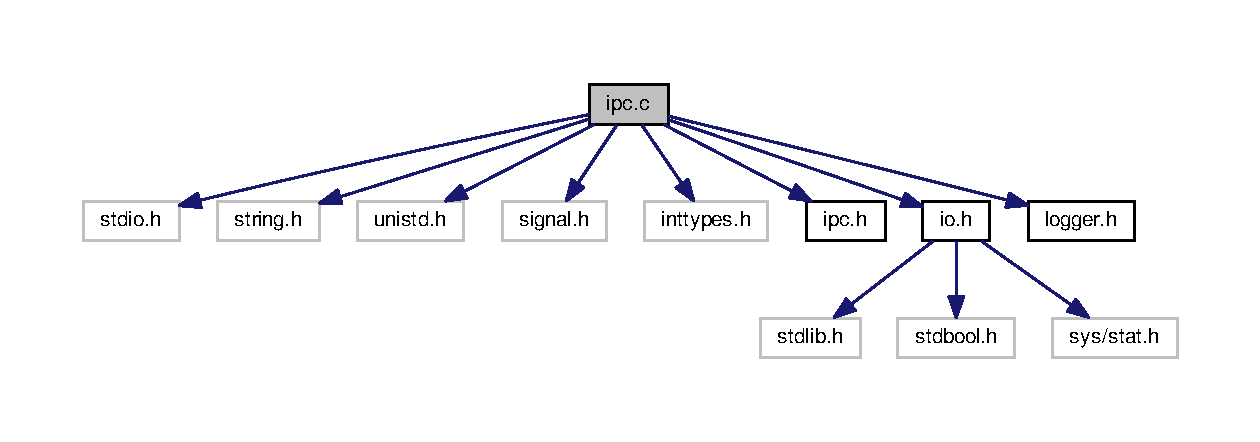
\includegraphics[width=350pt]{ipc_8c__incl}
\end{center}
\end{figure}
\subsection*{Macros}
\begin{DoxyCompactItemize}
\item 
\#define {\bfseries I\+P\+C\+\_\+\+M\+A\+X\+\_\+\+P\+I\+D\+\_\+\+S\+I\+ZE}~10\hypertarget{ipc_8c_a62451a7cf42dd8bb5d114bdd83b60520}{}\label{ipc_8c_a62451a7cf42dd8bb5d114bdd83b60520}

\item 
\#define {\bfseries I\+P\+C\+\_\+\+H\+O\+M\+E\+\_\+\+P\+A\+TH}~\char`\"{}/.searchfolder/\char`\"{}\hypertarget{ipc_8c_a000cc2e9e8132b15572f3e3ac63ebfde}{}\label{ipc_8c_a000cc2e9e8132b15572f3e3ac63ebfde}

\item 
\#define {\bfseries I\+P\+C\+\_\+\+R\+U\+N\+\_\+\+P\+A\+TH}~\char`\"{}/run/\char`\"{}\hypertarget{ipc_8c_a1d9abc515eaca8f30f4215eadb7417a2}{}\label{ipc_8c_a1d9abc515eaca8f30f4215eadb7417a2}

\item 
\#define {\bfseries I\+P\+C\+\_\+\+H\+O\+M\+E\+\_\+\+R\+U\+N\+\_\+\+P\+A\+TH}~I\+P\+C\+\_\+\+H\+O\+M\+E\+\_\+\+P\+A\+TH I\+P\+C\+\_\+\+R\+U\+N\+\_\+\+P\+A\+TH\hypertarget{ipc_8c_aa70926ca30ee98b193e64ef623f44556}{}\label{ipc_8c_aa70926ca30ee98b193e64ef623f44556}

\end{DoxyCompactItemize}
\subsection*{Functions}
\begin{DoxyCompactItemize}
\item 
static int \hyperlink{ipc_8c_a22de351993e78407550fe96832679286}{ipc\+\_\+get\+\_\+pid\+\_\+file\+\_\+path} (char $\ast$dst\+\_\+path, char $\ast$pid\+\_\+path)
\begin{DoxyCompactList}\small\item\em Return the pid file path for the watch constructed from the folder. \end{DoxyCompactList}\item 
void \hyperlink{ipc_8c_a3afaf4791a2c7adbc333713aa73a11a2}{ipc\+\_\+sig\+\_\+handler} ()\hypertarget{ipc_8c_a3afaf4791a2c7adbc333713aa73a11a2}{}\label{ipc_8c_a3afaf4791a2c7adbc333713aa73a11a2}

\begin{DoxyCompactList}\small\item\em I\+PC signal handler for S\+I\+G\+T\+E\+R\+M$\vert$\+S\+I\+G\+I\+NT that remove the watch and optionally call a callback. \end{DoxyCompactList}\item 
int \hyperlink{ipc_8c_a869a843644acd5eab7270099bc112a69}{ipc\+\_\+set\+\_\+watch} (char $\ast$dst\+\_\+path, ipc\+\_\+stop\+\_\+callback cb, void $\ast$cb\+\_\+arg)
\begin{DoxyCompactList}\small\item\em Create the instance run file for further identification by other instances, and setup signal catch. \end{DoxyCompactList}\item 
int \hyperlink{ipc_8c_a4f14d264fa040d8103d6e7a2f6088f44}{ipc\+\_\+remove\+\_\+watch} (char $\ast$dst\+\_\+path)
\begin{DoxyCompactList}\small\item\em Removes the watch file for the given search path. \end{DoxyCompactList}\item 
int \hyperlink{ipc_8c_a3cbaa8bad6fdc71f32bb803d628fcf25}{ipc\+\_\+stop\+\_\+watch} (char $\ast$dst\+\_\+path)
\begin{DoxyCompactList}\small\item\em Stop the instance designated by the given search path, using the S\+I\+G\+T\+E\+RM signal. \end{DoxyCompactList}\end{DoxyCompactItemize}
\subsection*{Variables}
\begin{DoxyCompactItemize}
\item 
static char \hyperlink{ipc_8c_aec456f2204fb2e615ce9e4884186e5f7}{g\+\_\+watch\+\_\+dst\+\_\+path} \mbox{[}\hyperlink{io_8h_a3459a8a15f99dc120380d828bc7a4cd8}{I\+O\+\_\+\+P\+A\+T\+H\+\_\+\+M\+A\+X\+\_\+\+S\+I\+ZE}\mbox{]} = \char`\"{}\char`\"{}\hypertarget{ipc_8c_aec456f2204fb2e615ce9e4884186e5f7}{}\label{ipc_8c_aec456f2204fb2e615ce9e4884186e5f7}

\begin{DoxyCompactList}\small\item\em Destination path on which this instance operates on. \end{DoxyCompactList}\item 
static ipc\+\_\+stop\+\_\+callback \hyperlink{ipc_8c_aa0e3adb6fceaeeb9422d6a46fdc30562}{g\+\_\+watch\+\_\+cb} = N\+U\+LL\hypertarget{ipc_8c_aa0e3adb6fceaeeb9422d6a46fdc30562}{}\label{ipc_8c_aa0e3adb6fceaeeb9422d6a46fdc30562}

\begin{DoxyCompactList}\small\item\em Provided callback when a signal is received. \end{DoxyCompactList}\item 
static void $\ast$ \hyperlink{ipc_8c_afc105ac7cbd447a0ab79b555cd65194f}{g\+\_\+watch\+\_\+cb\+\_\+arg} = N\+U\+LL\hypertarget{ipc_8c_afc105ac7cbd447a0ab79b555cd65194f}{}\label{ipc_8c_afc105ac7cbd447a0ab79b555cd65194f}

\begin{DoxyCompactList}\small\item\em Callback data for the callback when signal is received. \end{DoxyCompactList}\end{DoxyCompactItemize}


\subsection{Detailed Description}
Manage communication between different instance of smartfolder. 

In order to do this, during initialisation (ipc\+\_\+set\+\_\+watch), it create a file in the user home directory and put the P\+ID of the current instance in it. The name of this file is constructed by taking the provided destination path and replacing all directory separator by an underscore.

It also setup two signals catch (S\+I\+G\+I\+NT and S\+I\+G\+T\+E\+RM) for cleanup purpose. The callback and callback data are provided by the caller, and stored as global for usage in the signl handler. This is this handler that also remove the file in the user home directory.

Now, to terminate an instance, it gets the P\+ID of the target instance by getting it in the concerned file. To get this file, it does the same string replacement in the provided destination folder to have the right name. Then, with the P\+ID, it launch a S\+I\+G\+T\+E\+RM signal to the instance.

When a signal is received, the signal handler will first remove the file and call the callback if any.

\begin{DoxyAuthor}{Author}
Claudio Sousa, Gonzalez David 
\end{DoxyAuthor}


\subsection{Function Documentation}
\index{ipc.\+c@{ipc.\+c}!ipc\+\_\+get\+\_\+pid\+\_\+file\+\_\+path@{ipc\+\_\+get\+\_\+pid\+\_\+file\+\_\+path}}
\index{ipc\+\_\+get\+\_\+pid\+\_\+file\+\_\+path@{ipc\+\_\+get\+\_\+pid\+\_\+file\+\_\+path}!ipc.\+c@{ipc.\+c}}
\subsubsection[{\texorpdfstring{ipc\+\_\+get\+\_\+pid\+\_\+file\+\_\+path(char $\ast$dst\+\_\+path, char $\ast$pid\+\_\+path)}{ipc_get_pid_file_path(char *dst_path, char *pid_path)}}]{\setlength{\rightskip}{0pt plus 5cm}static int ipc\+\_\+get\+\_\+pid\+\_\+file\+\_\+path (
\begin{DoxyParamCaption}
\item[{char $\ast$}]{dst\+\_\+path, }
\item[{char $\ast$}]{pid\+\_\+path}
\end{DoxyParamCaption}
)\hspace{0.3cm}{\ttfamily [static]}}\hypertarget{ipc_8c_a22de351993e78407550fe96832679286}{}\label{ipc_8c_a22de351993e78407550fe96832679286}


Return the pid file path for the watch constructed from the folder. 

The pid filename is constructed by simply replacing the \textquotesingle{}/\textquotesingle{} character by \textquotesingle{}\+\_\+\textquotesingle{} 
\begin{DoxyParams}{Parameters}
{\em dst\+\_\+path} & The destination path to construct the filename from \\
\hline
{\em pid\+\_\+path} & String to store the resulting pid filename \\
\hline
\end{DoxyParams}


Definition at line 59 of file ipc.\+c.

\index{ipc.\+c@{ipc.\+c}!ipc\+\_\+remove\+\_\+watch@{ipc\+\_\+remove\+\_\+watch}}
\index{ipc\+\_\+remove\+\_\+watch@{ipc\+\_\+remove\+\_\+watch}!ipc.\+c@{ipc.\+c}}
\subsubsection[{\texorpdfstring{ipc\+\_\+remove\+\_\+watch(char $\ast$dst\+\_\+path)}{ipc_remove_watch(char *dst_path)}}]{\setlength{\rightskip}{0pt plus 5cm}int ipc\+\_\+remove\+\_\+watch (
\begin{DoxyParamCaption}
\item[{char $\ast$}]{dst\+\_\+path}
\end{DoxyParamCaption}
)}\hypertarget{ipc_8c_a4f14d264fa040d8103d6e7a2f6088f44}{}\label{ipc_8c_a4f14d264fa040d8103d6e7a2f6088f44}


Removes the watch file for the given search path. 


\begin{DoxyParams}{Parameters}
{\em dst\+\_\+path} & The destination path that designate the instance \\
\hline
\end{DoxyParams}
\begin{DoxyReturn}{Returns}
Error indicator\+: 0 for OK, 1 for an error 
\end{DoxyReturn}


Definition at line 132 of file ipc.\+c.

\index{ipc.\+c@{ipc.\+c}!ipc\+\_\+set\+\_\+watch@{ipc\+\_\+set\+\_\+watch}}
\index{ipc\+\_\+set\+\_\+watch@{ipc\+\_\+set\+\_\+watch}!ipc.\+c@{ipc.\+c}}
\subsubsection[{\texorpdfstring{ipc\+\_\+set\+\_\+watch(char $\ast$dst\+\_\+path, ipc\+\_\+stop\+\_\+callback cb, void $\ast$cb\+\_\+arg)}{ipc_set_watch(char *dst_path, ipc_stop_callback cb, void *cb_arg)}}]{\setlength{\rightskip}{0pt plus 5cm}int ipc\+\_\+set\+\_\+watch (
\begin{DoxyParamCaption}
\item[{char $\ast$}]{dst\+\_\+path, }
\item[{ipc\+\_\+stop\+\_\+callback}]{cb, }
\item[{void $\ast$}]{cb\+\_\+arg}
\end{DoxyParamCaption}
)}\hypertarget{ipc_8c_a869a843644acd5eab7270099bc112a69}{}\label{ipc_8c_a869a843644acd5eab7270099bc112a69}


Create the instance run file for further identification by other instances, and setup signal catch. 


\begin{DoxyParams}{Parameters}
{\em dst\+\_\+path} & The destination path this instance operates on \\
\hline
{\em cb} & Callback when a stop signal is received \\
\hline
{\em cb\+\_\+arg} & Callback argument \\
\hline
\end{DoxyParams}
\begin{DoxyReturn}{Returns}
Error indicator\+: 0 for OK, 1 for an error 
\end{DoxyReturn}


Definition at line 92 of file ipc.\+c.

\index{ipc.\+c@{ipc.\+c}!ipc\+\_\+stop\+\_\+watch@{ipc\+\_\+stop\+\_\+watch}}
\index{ipc\+\_\+stop\+\_\+watch@{ipc\+\_\+stop\+\_\+watch}!ipc.\+c@{ipc.\+c}}
\subsubsection[{\texorpdfstring{ipc\+\_\+stop\+\_\+watch(char $\ast$dst\+\_\+path)}{ipc_stop_watch(char *dst_path)}}]{\setlength{\rightskip}{0pt plus 5cm}int ipc\+\_\+stop\+\_\+watch (
\begin{DoxyParamCaption}
\item[{char $\ast$}]{dst\+\_\+path}
\end{DoxyParamCaption}
)}\hypertarget{ipc_8c_a3cbaa8bad6fdc71f32bb803d628fcf25}{}\label{ipc_8c_a3cbaa8bad6fdc71f32bb803d628fcf25}


Stop the instance designated by the given search path, using the S\+I\+G\+T\+E\+RM signal. 


\begin{DoxyParams}{Parameters}
{\em dst\+\_\+path} & The destination path that designate the instance \\
\hline
\end{DoxyParams}
\begin{DoxyReturn}{Returns}
Error indicator\+: 0 for OK, 1 for an error 
\end{DoxyReturn}


Definition at line 146 of file ipc.\+c.


\hypertarget{ipc_8h}{}\section{ipc.\+h File Reference}
\label{ipc_8h}\index{ipc.\+h@{ipc.\+h}}


Manage communication between different instance of smartfolder.  


This graph shows which files directly or indirectly include this file\+:\nopagebreak
\begin{figure}[H]
\begin{center}
\leavevmode
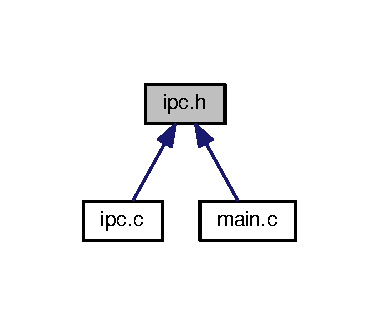
\includegraphics[width=182pt]{ipc_8h__dep__incl}
\end{center}
\end{figure}
\subsection*{Typedefs}
\begin{DoxyCompactItemize}
\item 
typedef void($\ast$ {\bfseries ipc\+\_\+stop\+\_\+callback}) (void $\ast$)\hypertarget{ipc_8h_a411bc98eff907bee7fb3371d08bf48db}{}\label{ipc_8h_a411bc98eff907bee7fb3371d08bf48db}

\end{DoxyCompactItemize}
\subsection*{Functions}
\begin{DoxyCompactItemize}
\item 
int \hyperlink{ipc_8h_a869a843644acd5eab7270099bc112a69}{ipc\+\_\+set\+\_\+watch} (char $\ast$dst\+\_\+path, ipc\+\_\+stop\+\_\+callback cb, void $\ast$cb\+\_\+arg)
\begin{DoxyCompactList}\small\item\em Create the instance run file for further identification by other instances, and setup signal catch. \end{DoxyCompactList}\item 
int \hyperlink{ipc_8h_a4f14d264fa040d8103d6e7a2f6088f44}{ipc\+\_\+remove\+\_\+watch} (char $\ast$dst\+\_\+path)
\begin{DoxyCompactList}\small\item\em Removes the watch file for the given search path. \end{DoxyCompactList}\item 
int \hyperlink{ipc_8h_a3cbaa8bad6fdc71f32bb803d628fcf25}{ipc\+\_\+stop\+\_\+watch} (char $\ast$dst\+\_\+path)
\begin{DoxyCompactList}\small\item\em Stop the instance designated by the given search path, using the S\+I\+G\+T\+E\+RM signal. \end{DoxyCompactList}\end{DoxyCompactItemize}


\subsection{Detailed Description}
Manage communication between different instance of smartfolder. 

In order to do this, during initialisation (ipc\+\_\+set\+\_\+watch), it create a file in the user home directory and put the P\+ID of the current instance in it. The name of this file is constructed by taking the provided destination path and replacing all directory separator by an underscore.

It also setup two signals catch (S\+I\+G\+I\+NT and S\+I\+G\+T\+E\+RM) for cleanup purpose. The callback and callback data are provided by the caller, and stored as global for usage in the signl handler. This is this handler that also remove the file in the user home directory.

Now, to terminate an instance, it gets the P\+ID of the target instance by getting it in the concerned file. To get this file, it does the same string replacement in the provided destination folder to have the right name. Then, with the P\+ID, it launch a S\+I\+G\+T\+E\+RM signal to the instance.

When a signal is received, the signal handler will first remove the file and call the callback if any.

\begin{DoxyAuthor}{Author}
Claudio Sousa, Gonzalez David 
\end{DoxyAuthor}


\subsection{Function Documentation}
\index{ipc.\+h@{ipc.\+h}!ipc\+\_\+remove\+\_\+watch@{ipc\+\_\+remove\+\_\+watch}}
\index{ipc\+\_\+remove\+\_\+watch@{ipc\+\_\+remove\+\_\+watch}!ipc.\+h@{ipc.\+h}}
\subsubsection[{\texorpdfstring{ipc\+\_\+remove\+\_\+watch(char $\ast$dst\+\_\+path)}{ipc_remove_watch(char *dst_path)}}]{\setlength{\rightskip}{0pt plus 5cm}int ipc\+\_\+remove\+\_\+watch (
\begin{DoxyParamCaption}
\item[{char $\ast$}]{dst\+\_\+path}
\end{DoxyParamCaption}
)}\hypertarget{ipc_8h_a4f14d264fa040d8103d6e7a2f6088f44}{}\label{ipc_8h_a4f14d264fa040d8103d6e7a2f6088f44}


Removes the watch file for the given search path. 


\begin{DoxyParams}{Parameters}
{\em dst\+\_\+path} & The destination path that designate the instance \\
\hline
\end{DoxyParams}
\begin{DoxyReturn}{Returns}
Error indicator\+: 0 for OK, 1 for an error 
\end{DoxyReturn}


Definition at line 132 of file ipc.\+c.

\index{ipc.\+h@{ipc.\+h}!ipc\+\_\+set\+\_\+watch@{ipc\+\_\+set\+\_\+watch}}
\index{ipc\+\_\+set\+\_\+watch@{ipc\+\_\+set\+\_\+watch}!ipc.\+h@{ipc.\+h}}
\subsubsection[{\texorpdfstring{ipc\+\_\+set\+\_\+watch(char $\ast$dst\+\_\+path, ipc\+\_\+stop\+\_\+callback cb, void $\ast$cb\+\_\+arg)}{ipc_set_watch(char *dst_path, ipc_stop_callback cb, void *cb_arg)}}]{\setlength{\rightskip}{0pt plus 5cm}int ipc\+\_\+set\+\_\+watch (
\begin{DoxyParamCaption}
\item[{char $\ast$}]{dst\+\_\+path, }
\item[{ipc\+\_\+stop\+\_\+callback}]{cb, }
\item[{void $\ast$}]{cb\+\_\+arg}
\end{DoxyParamCaption}
)}\hypertarget{ipc_8h_a869a843644acd5eab7270099bc112a69}{}\label{ipc_8h_a869a843644acd5eab7270099bc112a69}


Create the instance run file for further identification by other instances, and setup signal catch. 


\begin{DoxyParams}{Parameters}
{\em dst\+\_\+path} & The destination path this instance operates on \\
\hline
{\em cb} & Callback when a stop signal is received \\
\hline
{\em cb\+\_\+arg} & Callback argument \\
\hline
\end{DoxyParams}
\begin{DoxyReturn}{Returns}
Error indicator\+: 0 for OK, 1 for an error 
\end{DoxyReturn}


Definition at line 92 of file ipc.\+c.

\index{ipc.\+h@{ipc.\+h}!ipc\+\_\+stop\+\_\+watch@{ipc\+\_\+stop\+\_\+watch}}
\index{ipc\+\_\+stop\+\_\+watch@{ipc\+\_\+stop\+\_\+watch}!ipc.\+h@{ipc.\+h}}
\subsubsection[{\texorpdfstring{ipc\+\_\+stop\+\_\+watch(char $\ast$dst\+\_\+path)}{ipc_stop_watch(char *dst_path)}}]{\setlength{\rightskip}{0pt plus 5cm}int ipc\+\_\+stop\+\_\+watch (
\begin{DoxyParamCaption}
\item[{char $\ast$}]{dst\+\_\+path}
\end{DoxyParamCaption}
)}\hypertarget{ipc_8h_a3cbaa8bad6fdc71f32bb803d628fcf25}{}\label{ipc_8h_a3cbaa8bad6fdc71f32bb803d628fcf25}


Stop the instance designated by the given search path, using the S\+I\+G\+T\+E\+RM signal. 


\begin{DoxyParams}{Parameters}
{\em dst\+\_\+path} & The destination path that designate the instance \\
\hline
\end{DoxyParams}
\begin{DoxyReturn}{Returns}
Error indicator\+: 0 for OK, 1 for an error 
\end{DoxyReturn}


Definition at line 146 of file ipc.\+c.


\hypertarget{linker_8c}{}\section{linker.\+c File Reference}
\label{linker_8c}\index{linker.\+c@{linker.\+c}}


The linker maintains an updated list of links to the found files.  


{\ttfamily \#include $<$stdio.\+h$>$}\\*
{\ttfamily \#include $<$string.\+h$>$}\\*
{\ttfamily \#include $<$unistd.\+h$>$}\\*
{\ttfamily \#include $<$libgen.\+h$>$}\\*
{\ttfamily \#include \char`\"{}linker.\+h\char`\"{}}\\*
{\ttfamily \#include \char`\"{}io.\+h\char`\"{}}\\*
{\ttfamily \#include \char`\"{}logger.\+h\char`\"{}}\\*
Include dependency graph for linker.\+c\+:\nopagebreak
\begin{figure}[H]
\begin{center}
\leavevmode
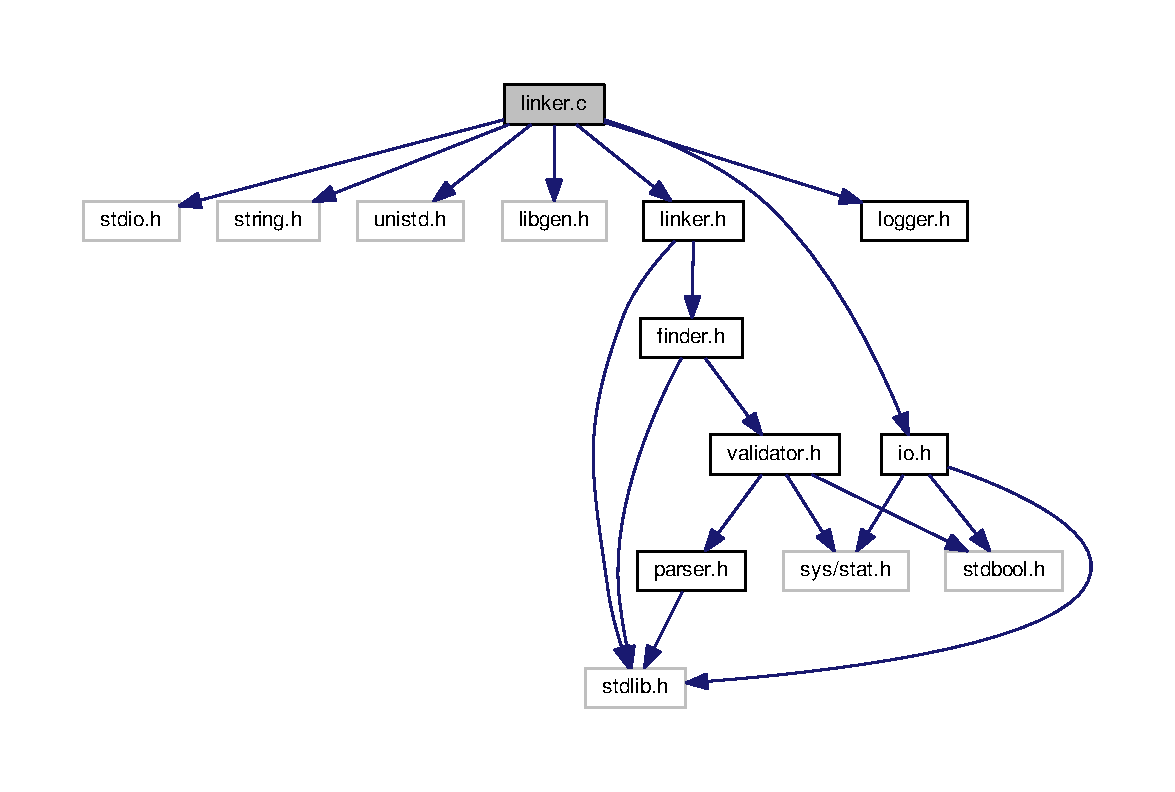
\includegraphics[width=350pt]{linker_8c__incl}
\end{center}
\end{figure}
\subsection*{Functions}
\begin{DoxyCompactItemize}
\item 
void \hyperlink{linker_8c_a2d26744c8bc9442c30314d61f19bb2b5}{linker\+\_\+purge} (char $\ast$dst\+\_\+path, \hyperlink{structfinder__t}{finder\+\_\+t} $\ast$\hyperlink{finder_8c_a8bb2e2bcd7c9c20c6bdf286c0c1b67e4}{files})
\begin{DoxyCompactList}\small\item\em Delete all links in the destination folder that are no longer in the given list. \end{DoxyCompactList}\item 
void \hyperlink{linker_8c_a03bffbdcce1d8af640bd0cac561dfdae}{linker\+\_\+update} (char $\ast$dst\+\_\+path, \hyperlink{structfinder__t}{finder\+\_\+t} $\ast$\hyperlink{finder_8c_a8bb2e2bcd7c9c20c6bdf286c0c1b67e4}{files})
\begin{DoxyCompactList}\small\item\em Update the links in the destination folder (create new ones and purge older ones). \end{DoxyCompactList}\end{DoxyCompactItemize}


\subsection{Detailed Description}
The linker maintains an updated list of links to the found files. 

The linker has two jobs\+:
\begin{DoxyItemize}
\item creates the links for the provided list of files found;
\item deletes old links that are no longer present in the list.
\end{DoxyItemize}

In order to create the links, it simply take the base name of the target file and create the link with this name in the destination folder. But to manage duplicate, it count the number of files that has the same basename in the list before the current one and if it is not 0, append the number to the name.

To purge the destination folder, it gets all the links in it. Then, for each link, it determines whether a file is no longer here by searching the target of the link in the list. If it is not found, the linker deletes the link in the destination folder.

\begin{DoxyAuthor}{Author}
Claudio Sousa, Gonzalez David 
\end{DoxyAuthor}


\subsection{Function Documentation}
\index{linker.\+c@{linker.\+c}!linker\+\_\+purge@{linker\+\_\+purge}}
\index{linker\+\_\+purge@{linker\+\_\+purge}!linker.\+c@{linker.\+c}}
\subsubsection[{\texorpdfstring{linker\+\_\+purge(char $\ast$dst\+\_\+path, finder\+\_\+t $\ast$files)}{linker_purge(char *dst_path, finder_t *files)}}]{\setlength{\rightskip}{0pt plus 5cm}void linker\+\_\+purge (
\begin{DoxyParamCaption}
\item[{char $\ast$}]{dst\+\_\+path, }
\item[{{\bf finder\+\_\+t} $\ast$}]{files}
\end{DoxyParamCaption}
)}\hypertarget{linker_8c_a2d26744c8bc9442c30314d61f19bb2b5}{}\label{linker_8c_a2d26744c8bc9442c30314d61f19bb2b5}


Delete all links in the destination folder that are no longer in the given list. 

To determine whether a file is no longer here, it searchs the target of the link in the list. If it is not found, the linker delete the link. 
\begin{DoxyParams}{Parameters}
{\em dst\+\_\+path} & Where to put the links \\
\hline
{\em files} & List of files to link \\
\hline
\end{DoxyParams}


Definition at line 36 of file linker.\+c.

\index{linker.\+c@{linker.\+c}!linker\+\_\+update@{linker\+\_\+update}}
\index{linker\+\_\+update@{linker\+\_\+update}!linker.\+c@{linker.\+c}}
\subsubsection[{\texorpdfstring{linker\+\_\+update(char $\ast$dst\+\_\+path, finder\+\_\+t $\ast$files)}{linker_update(char *dst_path, finder_t *files)}}]{\setlength{\rightskip}{0pt plus 5cm}void linker\+\_\+update (
\begin{DoxyParamCaption}
\item[{char $\ast$}]{dst\+\_\+path, }
\item[{{\bf finder\+\_\+t} $\ast$}]{files}
\end{DoxyParamCaption}
)}\hypertarget{linker_8c_a03bffbdcce1d8af640bd0cac561dfdae}{}\label{linker_8c_a03bffbdcce1d8af640bd0cac561dfdae}


Update the links in the destination folder (create new ones and purge older ones). 


\begin{DoxyParams}{Parameters}
{\em dst\+\_\+path} & Where to put the links \\
\hline
{\em files} & List of files to link \\
\hline
\end{DoxyParams}


Definition at line 66 of file linker.\+c.


\hypertarget{linker_8h}{}\section{linker.\+h File Reference}
\label{linker_8h}\index{linker.\+h@{linker.\+h}}


The linker maintains an updated list of links to the found files.  


{\ttfamily \#include $<$stdlib.\+h$>$}\\*
{\ttfamily \#include \char`\"{}finder.\+h\char`\"{}}\\*
Include dependency graph for linker.\+h\+:\nopagebreak
\begin{figure}[H]
\begin{center}
\leavevmode
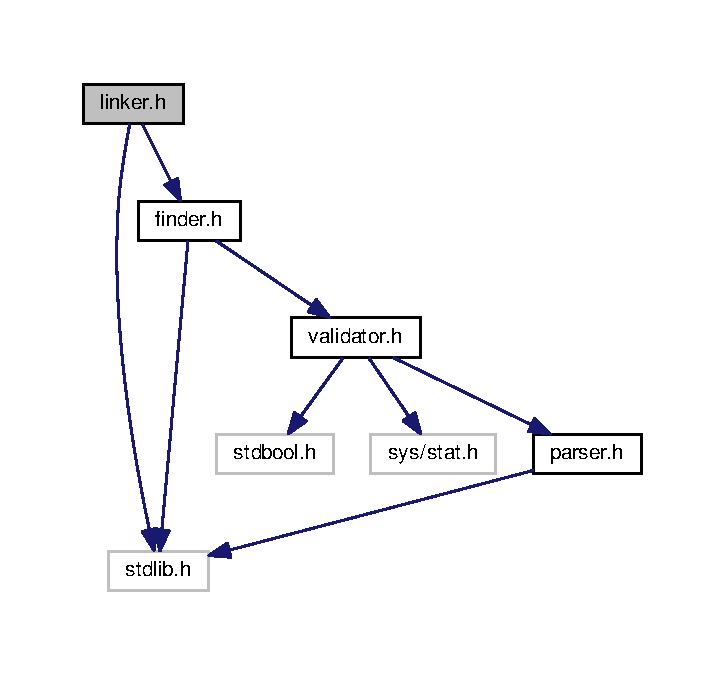
\includegraphics[width=348pt]{linker_8h__incl}
\end{center}
\end{figure}
This graph shows which files directly or indirectly include this file\+:
\nopagebreak
\begin{figure}[H]
\begin{center}
\leavevmode
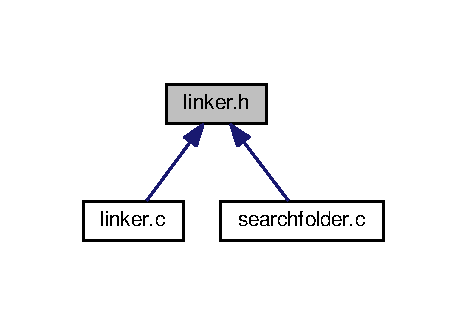
\includegraphics[width=224pt]{linker_8h__dep__incl}
\end{center}
\end{figure}
\subsection*{Functions}
\begin{DoxyCompactItemize}
\item 
void \hyperlink{linker_8h_a03bffbdcce1d8af640bd0cac561dfdae}{linker\+\_\+update} (char $\ast$dst\+\_\+path, \hyperlink{structfinder__t}{finder\+\_\+t} $\ast$files)
\begin{DoxyCompactList}\small\item\em Update the links in the destination folder (create new ones and purge older ones). \end{DoxyCompactList}\end{DoxyCompactItemize}


\subsection{Detailed Description}
The linker maintains an updated list of links to the found files. 

The linker has two jobs\+:
\begin{DoxyItemize}
\item creates the links for the provided list of files found;
\item deletes old links that are no longer present in the list.
\end{DoxyItemize}

In order to create the links, it simply take the base name of the target file and create the link with this name in the destination folder. But to manage duplicate, it count the number of files that has the same basename in the list before the current one and if it is not 0, append the number to the name.

To purge the destination folder, it gets all the links in it. Then, for each link, it determines whether a file is no longer here by searching the target of the link in the list. If it is not found, the linker deletes the link in the destination folder.

\begin{DoxyAuthor}{Author}
Claudio Sousa, Gonzalez David 
\end{DoxyAuthor}


\subsection{Function Documentation}
\index{linker.\+h@{linker.\+h}!linker\+\_\+update@{linker\+\_\+update}}
\index{linker\+\_\+update@{linker\+\_\+update}!linker.\+h@{linker.\+h}}
\subsubsection[{\texorpdfstring{linker\+\_\+update(char $\ast$dst\+\_\+path, finder\+\_\+t $\ast$files)}{linker_update(char *dst_path, finder_t *files)}}]{\setlength{\rightskip}{0pt plus 5cm}void linker\+\_\+update (
\begin{DoxyParamCaption}
\item[{char $\ast$}]{dst\+\_\+path, }
\item[{{\bf finder\+\_\+t} $\ast$}]{files}
\end{DoxyParamCaption}
)}\hypertarget{linker_8h_a03bffbdcce1d8af640bd0cac561dfdae}{}\label{linker_8h_a03bffbdcce1d8af640bd0cac561dfdae}


Update the links in the destination folder (create new ones and purge older ones). 


\begin{DoxyParams}{Parameters}
{\em dst\+\_\+path} & Where to put the links \\
\hline
{\em files} & List of files to link \\
\hline
\end{DoxyParams}


Definition at line 66 of file linker.\+c.


\hypertarget{logger_8c}{}\section{logger.\+c File Reference}
\label{logger_8c}\index{logger.\+c@{logger.\+c}}


Simple logger functions that allow logging of various informations and errors.  


{\ttfamily \#include $<$stdio.\+h$>$}\\*
{\ttfamily \#include $<$unistd.\+h$>$}\\*
{\ttfamily \#include $<$stdarg.\+h$>$}\\*
{\ttfamily \#include $<$errno.\+h$>$}\\*
{\ttfamily \#include $<$string.\+h$>$}\\*
{\ttfamily \#include \char`\"{}logger.\+h\char`\"{}}\\*
{\ttfamily \#include \char`\"{}io.\+h\char`\"{}}\\*
Include dependency graph for logger.\+c\+:\nopagebreak
\begin{figure}[H]
\begin{center}
\leavevmode
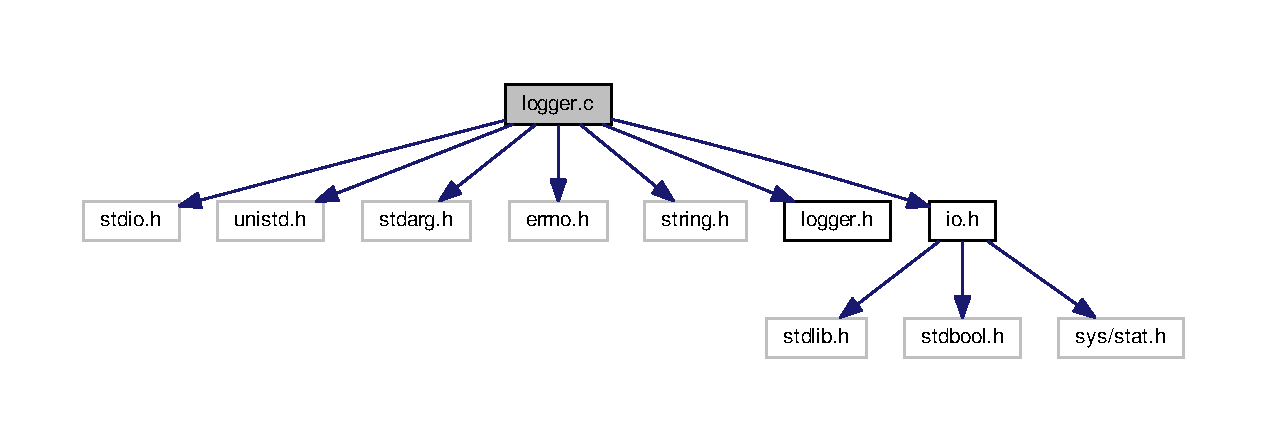
\includegraphics[width=350pt]{logger_8c__incl}
\end{center}
\end{figure}
\subsection*{Macros}
\begin{DoxyCompactItemize}
\item 
\#define {\bfseries L\+O\+G\+G\+E\+R\+\_\+\+M\+S\+G\+\_\+\+M\+AX}~256\hypertarget{logger_8c_a862c89f441ad8b4a6c2249b0ef3effe7}{}\label{logger_8c_a862c89f441ad8b4a6c2249b0ef3effe7}

\end{DoxyCompactItemize}
\subsection*{Functions}
\begin{DoxyCompactItemize}
\item 
void \hyperlink{logger_8c_a31cd41f12696a1cfa8f3d0ee7271eacd}{logger\+\_\+debug} (char $\ast$fmt,...)
\begin{DoxyCompactList}\small\item\em Log a message on S\+T\+D\+O\+UT if debug mode is enabled. \end{DoxyCompactList}\item 
void \hyperlink{logger_8c_a251077259cd16790866368555b1ade54}{logger\+\_\+info} (char $\ast$fmt,...)
\begin{DoxyCompactList}\small\item\em Log a message on S\+T\+D\+O\+UT. \end{DoxyCompactList}\item 
void \hyperlink{logger_8c_ae3babed41be6499526f89c1acf2ec37f}{logger\+\_\+error} (char $\ast$fmt,...)
\begin{DoxyCompactList}\small\item\em Log an error message on S\+T\+D\+E\+RR. \end{DoxyCompactList}\item 
void \hyperlink{logger_8c_a8fea334aadc9bc5d968de863481b5f0a}{logger\+\_\+perror} (char $\ast$msg)
\begin{DoxyCompactList}\small\item\em Log an error message on S\+T\+D\+E\+RR using perror (P\+O\+S\+IX) \end{DoxyCompactList}\end{DoxyCompactItemize}


\subsection{Detailed Description}
Simple logger functions that allow logging of various informations and errors. 

\begin{DoxyAuthor}{Author}
Claudio Sousa, Gonzalez David 
\end{DoxyAuthor}


\subsection{Function Documentation}
\index{logger.\+c@{logger.\+c}!logger\+\_\+debug@{logger\+\_\+debug}}
\index{logger\+\_\+debug@{logger\+\_\+debug}!logger.\+c@{logger.\+c}}
\subsubsection[{\texorpdfstring{logger\+\_\+debug(char $\ast$fmt,...)}{logger_debug(char *fmt,...)}}]{\setlength{\rightskip}{0pt plus 5cm}void logger\+\_\+debug (
\begin{DoxyParamCaption}
\item[{char $\ast$}]{fmt, }
\item[{}]{...}
\end{DoxyParamCaption}
)}\hypertarget{logger_8c_a31cd41f12696a1cfa8f3d0ee7271eacd}{}\label{logger_8c_a31cd41f12696a1cfa8f3d0ee7271eacd}


Log a message on S\+T\+D\+O\+UT if debug mode is enabled. 


\begin{DoxyParams}{Parameters}
{\em fmt} & Message to log with printf() format allowed \\
\hline
{\em ...} & Format args \\
\hline
\end{DoxyParams}


Definition at line 17 of file logger.\+c.

\index{logger.\+c@{logger.\+c}!logger\+\_\+error@{logger\+\_\+error}}
\index{logger\+\_\+error@{logger\+\_\+error}!logger.\+c@{logger.\+c}}
\subsubsection[{\texorpdfstring{logger\+\_\+error(char $\ast$fmt,...)}{logger_error(char *fmt,...)}}]{\setlength{\rightskip}{0pt plus 5cm}void logger\+\_\+error (
\begin{DoxyParamCaption}
\item[{char $\ast$}]{fmt, }
\item[{}]{...}
\end{DoxyParamCaption}
)}\hypertarget{logger_8c_ae3babed41be6499526f89c1acf2ec37f}{}\label{logger_8c_ae3babed41be6499526f89c1acf2ec37f}


Log an error message on S\+T\+D\+E\+RR. 


\begin{DoxyParams}{Parameters}
{\em fmt} & Message to log with printf() format allowed \\
\hline
{\em ...} & Format args \\
\hline
\end{DoxyParams}


Definition at line 43 of file logger.\+c.

\index{logger.\+c@{logger.\+c}!logger\+\_\+info@{logger\+\_\+info}}
\index{logger\+\_\+info@{logger\+\_\+info}!logger.\+c@{logger.\+c}}
\subsubsection[{\texorpdfstring{logger\+\_\+info(char $\ast$fmt,...)}{logger_info(char *fmt,...)}}]{\setlength{\rightskip}{0pt plus 5cm}void logger\+\_\+info (
\begin{DoxyParamCaption}
\item[{char $\ast$}]{fmt, }
\item[{}]{...}
\end{DoxyParamCaption}
)}\hypertarget{logger_8c_a251077259cd16790866368555b1ade54}{}\label{logger_8c_a251077259cd16790866368555b1ade54}


Log a message on S\+T\+D\+O\+UT. 


\begin{DoxyParams}{Parameters}
{\em fmt} & Message to log with printf() format allowed \\
\hline
{\em ...} & Format args \\
\hline
\end{DoxyParams}


Definition at line 32 of file logger.\+c.

\index{logger.\+c@{logger.\+c}!logger\+\_\+perror@{logger\+\_\+perror}}
\index{logger\+\_\+perror@{logger\+\_\+perror}!logger.\+c@{logger.\+c}}
\subsubsection[{\texorpdfstring{logger\+\_\+perror(char $\ast$msg)}{logger_perror(char *msg)}}]{\setlength{\rightskip}{0pt plus 5cm}void logger\+\_\+perror (
\begin{DoxyParamCaption}
\item[{char $\ast$}]{msg}
\end{DoxyParamCaption}
)}\hypertarget{logger_8c_a8fea334aadc9bc5d968de863481b5f0a}{}\label{logger_8c_a8fea334aadc9bc5d968de863481b5f0a}


Log an error message on S\+T\+D\+E\+RR using perror (P\+O\+S\+IX) 


\begin{DoxyParams}{Parameters}
{\em msg} & Message to log \\
\hline
\end{DoxyParams}


Definition at line 54 of file logger.\+c.


\hypertarget{logger_8h}{}\section{logger.\+h File Reference}
\label{logger_8h}\index{logger.\+h@{logger.\+h}}


Simple logger functions that allow logging of various informations and errors.  


This graph shows which files directly or indirectly include this file\+:
\nopagebreak
\begin{figure}[H]
\begin{center}
\leavevmode
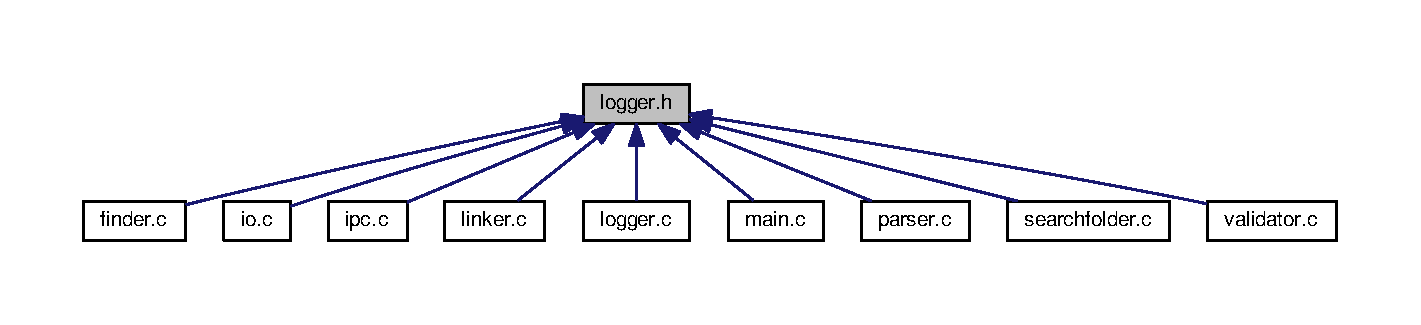
\includegraphics[width=350pt]{logger_8h__dep__incl}
\end{center}
\end{figure}
\subsection*{Functions}
\begin{DoxyCompactItemize}
\item 
void \hyperlink{logger_8h_a31cd41f12696a1cfa8f3d0ee7271eacd}{logger\+\_\+debug} (char $\ast$fmt,...)
\begin{DoxyCompactList}\small\item\em Log a message on S\+T\+D\+O\+UT if debug mode is enabled. \end{DoxyCompactList}\item 
void \hyperlink{logger_8h_a251077259cd16790866368555b1ade54}{logger\+\_\+info} (char $\ast$fmt,...)
\begin{DoxyCompactList}\small\item\em Log a message on S\+T\+D\+O\+UT. \end{DoxyCompactList}\item 
void \hyperlink{logger_8h_ae3babed41be6499526f89c1acf2ec37f}{logger\+\_\+error} (char $\ast$fmt,...)
\begin{DoxyCompactList}\small\item\em Log an error message on S\+T\+D\+E\+RR. \end{DoxyCompactList}\item 
void \hyperlink{logger_8h_a8fea334aadc9bc5d968de863481b5f0a}{logger\+\_\+perror} (char $\ast$msg)
\begin{DoxyCompactList}\small\item\em Log an error message on S\+T\+D\+E\+RR using perror (P\+O\+S\+IX) \end{DoxyCompactList}\end{DoxyCompactItemize}


\subsection{Detailed Description}
Simple logger functions that allow logging of various informations and errors. 

\begin{DoxyAuthor}{Author}
Claudio Sousa, Gonzalez David 
\end{DoxyAuthor}


\subsection{Function Documentation}
\index{logger.\+h@{logger.\+h}!logger\+\_\+debug@{logger\+\_\+debug}}
\index{logger\+\_\+debug@{logger\+\_\+debug}!logger.\+h@{logger.\+h}}
\subsubsection[{\texorpdfstring{logger\+\_\+debug(char $\ast$fmt,...)}{logger_debug(char *fmt,...)}}]{\setlength{\rightskip}{0pt plus 5cm}void logger\+\_\+debug (
\begin{DoxyParamCaption}
\item[{char $\ast$}]{fmt, }
\item[{}]{...}
\end{DoxyParamCaption}
)}\hypertarget{logger_8h_a31cd41f12696a1cfa8f3d0ee7271eacd}{}\label{logger_8h_a31cd41f12696a1cfa8f3d0ee7271eacd}


Log a message on S\+T\+D\+O\+UT if debug mode is enabled. 


\begin{DoxyParams}{Parameters}
{\em fmt} & Message to log with printf() format allowed \\
\hline
{\em ...} & Format args \\
\hline
\end{DoxyParams}


Definition at line 17 of file logger.\+c.

\index{logger.\+h@{logger.\+h}!logger\+\_\+error@{logger\+\_\+error}}
\index{logger\+\_\+error@{logger\+\_\+error}!logger.\+h@{logger.\+h}}
\subsubsection[{\texorpdfstring{logger\+\_\+error(char $\ast$fmt,...)}{logger_error(char *fmt,...)}}]{\setlength{\rightskip}{0pt plus 5cm}void logger\+\_\+error (
\begin{DoxyParamCaption}
\item[{char $\ast$}]{fmt, }
\item[{}]{...}
\end{DoxyParamCaption}
)}\hypertarget{logger_8h_ae3babed41be6499526f89c1acf2ec37f}{}\label{logger_8h_ae3babed41be6499526f89c1acf2ec37f}


Log an error message on S\+T\+D\+E\+RR. 


\begin{DoxyParams}{Parameters}
{\em fmt} & Message to log with printf() format allowed \\
\hline
{\em ...} & Format args \\
\hline
\end{DoxyParams}


Definition at line 43 of file logger.\+c.

\index{logger.\+h@{logger.\+h}!logger\+\_\+info@{logger\+\_\+info}}
\index{logger\+\_\+info@{logger\+\_\+info}!logger.\+h@{logger.\+h}}
\subsubsection[{\texorpdfstring{logger\+\_\+info(char $\ast$fmt,...)}{logger_info(char *fmt,...)}}]{\setlength{\rightskip}{0pt plus 5cm}void logger\+\_\+info (
\begin{DoxyParamCaption}
\item[{char $\ast$}]{fmt, }
\item[{}]{...}
\end{DoxyParamCaption}
)}\hypertarget{logger_8h_a251077259cd16790866368555b1ade54}{}\label{logger_8h_a251077259cd16790866368555b1ade54}


Log a message on S\+T\+D\+O\+UT. 


\begin{DoxyParams}{Parameters}
{\em fmt} & Message to log with printf() format allowed \\
\hline
{\em ...} & Format args \\
\hline
\end{DoxyParams}


Definition at line 32 of file logger.\+c.

\index{logger.\+h@{logger.\+h}!logger\+\_\+perror@{logger\+\_\+perror}}
\index{logger\+\_\+perror@{logger\+\_\+perror}!logger.\+h@{logger.\+h}}
\subsubsection[{\texorpdfstring{logger\+\_\+perror(char $\ast$msg)}{logger_perror(char *msg)}}]{\setlength{\rightskip}{0pt plus 5cm}void logger\+\_\+perror (
\begin{DoxyParamCaption}
\item[{char $\ast$}]{msg}
\end{DoxyParamCaption}
)}\hypertarget{logger_8h_a8fea334aadc9bc5d968de863481b5f0a}{}\label{logger_8h_a8fea334aadc9bc5d968de863481b5f0a}


Log an error message on S\+T\+D\+E\+RR using perror (P\+O\+S\+IX) 


\begin{DoxyParams}{Parameters}
{\em msg} & Message to log \\
\hline
\end{DoxyParams}


Definition at line 54 of file logger.\+c.


\hypertarget{main_8c}{}\section{main.\+c File Reference}
\label{main_8c}\index{main.\+c@{main.\+c}}


Main program\+: deamonise, parse argument and launch the search.  


{\ttfamily \#include $<$stdio.\+h$>$}\\*
{\ttfamily \#include $<$stdlib.\+h$>$}\\*
{\ttfamily \#include $<$string.\+h$>$}\\*
{\ttfamily \#include $<$unistd.\+h$>$}\\*
{\ttfamily \#include \char`\"{}ipc.\+h\char`\"{}}\\*
{\ttfamily \#include \char`\"{}parser.\+h\char`\"{}}\\*
{\ttfamily \#include \char`\"{}searchfolder.\+h\char`\"{}}\\*
{\ttfamily \#include \char`\"{}io.\+h\char`\"{}}\\*
{\ttfamily \#include \char`\"{}logger.\+h\char`\"{}}\\*
Include dependency graph for main.\+c\+:\nopagebreak
\begin{figure}[H]
\begin{center}
\leavevmode
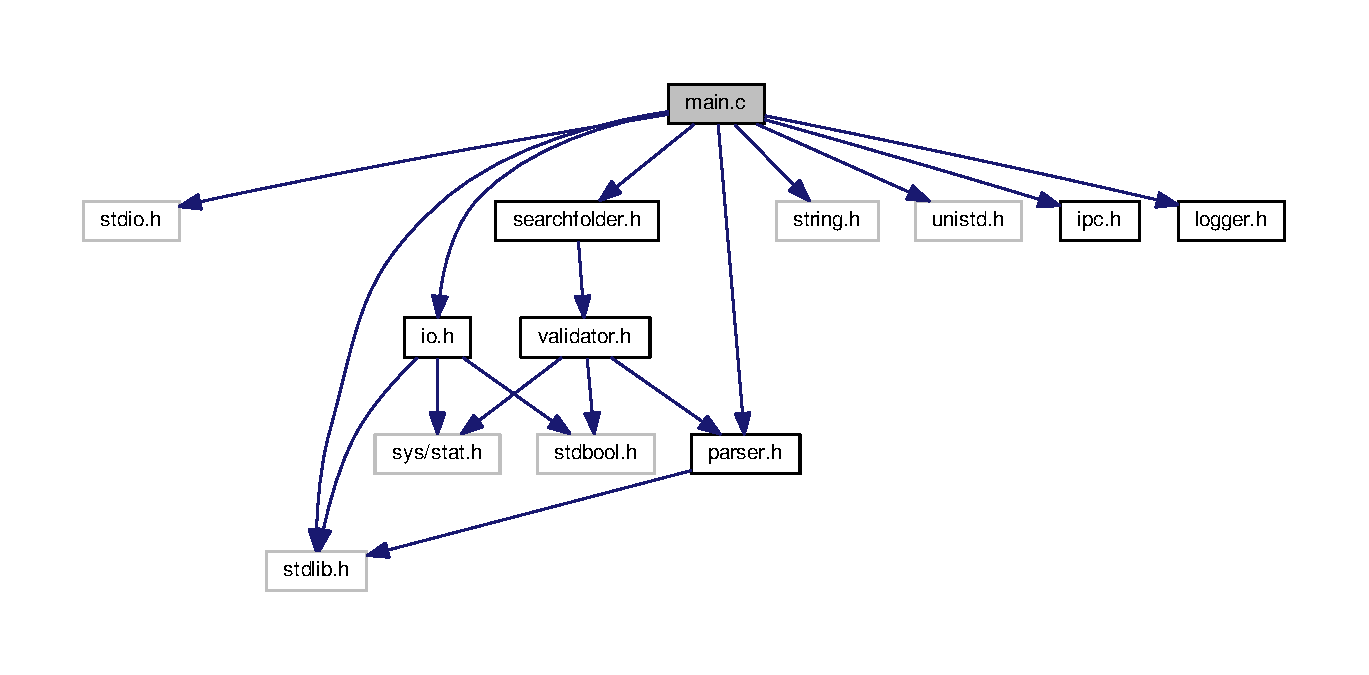
\includegraphics[width=350pt]{main_8c__incl}
\end{center}
\end{figure}
\subsection*{Functions}
\begin{DoxyCompactItemize}
\item 
void \hyperlink{main_8c_a5724b5d5bd1fb93f9ae44b8d46b64328}{print\+\_\+usage} (char $\ast$prog\+\_\+name)
\begin{DoxyCompactList}\small\item\em Prints program usage. \end{DoxyCompactList}\item 
int \hyperlink{main_8c_a0ddf1224851353fc92bfbff6f499fa97}{main} (int argc, char $\ast$argv\mbox{[}$\,$\mbox{]})
\begin{DoxyCompactList}\small\item\em Program entry-\/point. \end{DoxyCompactList}\end{DoxyCompactItemize}


\subsection{Detailed Description}
Main program\+: deamonise, parse argument and launch the search. 

Its role is to parse command-\/line arguments and\+:
\begin{DoxyItemize}
\item launch the parser to create the expression to validate against files;
\item set up the communication channel between instance;
\item launch the main searchfoler loop. Also, it can run in two mode\+:
\item normal\+: do what is above;
\item kill (-\/d)\+: use the communication channel to stop the designated instance. \begin{DoxyAuthor}{Author}
Claudio Sousa, Gonzalez David 
\end{DoxyAuthor}

\end{DoxyItemize}

\subsection{Function Documentation}
\index{main.\+c@{main.\+c}!main@{main}}
\index{main@{main}!main.\+c@{main.\+c}}
\subsubsection[{\texorpdfstring{main(int argc, char $\ast$argv[])}{main(int argc, char *argv[])}}]{\setlength{\rightskip}{0pt plus 5cm}int main (
\begin{DoxyParamCaption}
\item[{int}]{argc, }
\item[{char $\ast$}]{argv\mbox{[}$\,$\mbox{]}}
\end{DoxyParamCaption}
)}\hypertarget{main_8c_a0ddf1224851353fc92bfbff6f499fa97}{}\label{main_8c_a0ddf1224851353fc92bfbff6f499fa97}


Program entry-\/point. 


\begin{DoxyParams}{Parameters}
{\em argc} & Number of arguments \\
\hline
{\em argv} & Array of arguments \\
\hline
\end{DoxyParams}


Definition at line 41 of file main.\+c.

\index{main.\+c@{main.\+c}!print\+\_\+usage@{print\+\_\+usage}}
\index{print\+\_\+usage@{print\+\_\+usage}!main.\+c@{main.\+c}}
\subsubsection[{\texorpdfstring{print\+\_\+usage(char $\ast$prog\+\_\+name)}{print_usage(char *prog_name)}}]{\setlength{\rightskip}{0pt plus 5cm}void print\+\_\+usage (
\begin{DoxyParamCaption}
\item[{char $\ast$}]{prog\+\_\+name}
\end{DoxyParamCaption}
)}\hypertarget{main_8c_a5724b5d5bd1fb93f9ae44b8d46b64328}{}\label{main_8c_a5724b5d5bd1fb93f9ae44b8d46b64328}


Prints program usage. 


\begin{DoxyParams}{Parameters}
{\em prog\+\_\+name} & Program name \\
\hline
\end{DoxyParams}


Definition at line 28 of file main.\+c.


\hypertarget{parser_8c}{}\section{parser.\+c File Reference}
\label{parser_8c}\index{parser.\+c@{parser.\+c}}


Parses a string expression and return a formal representation.  


{\ttfamily \#include $<$string.\+h$>$}\\*
{\ttfamily \#include $<$stdlib.\+h$>$}\\*
{\ttfamily \#include $<$math.\+h$>$}\\*
{\ttfamily \#include $<$pwd.\+h$>$}\\*
{\ttfamily \#include $<$grp.\+h$>$}\\*
{\ttfamily \#include \char`\"{}parser.\+h\char`\"{}}\\*
{\ttfamily \#include \char`\"{}logger.\+h\char`\"{}}\\*
Include dependency graph for parser.\+c\+:\nopagebreak
\begin{figure}[H]
\begin{center}
\leavevmode
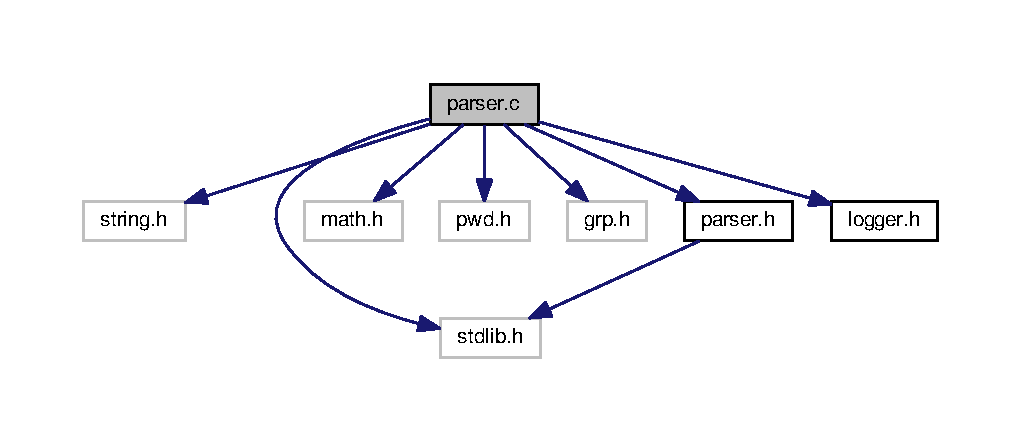
\includegraphics[width=350pt]{parser_8c__incl}
\end{center}
\end{figure}
\subsection*{Macros}
\begin{DoxyCompactItemize}
\item 
\#define \hyperlink{parser_8c_a20f8a4e237e6918372da5e1aec3426c8}{C\+R\+I\+T\+E\+R\+I\+A\+\_\+\+C\+O\+U\+NT}~8
\begin{DoxyCompactList}\small\item\em Number of criteria belonging to the C\+R\+I\+T\+E\+R\+IA criteria type. \end{DoxyCompactList}\item 
\#define \hyperlink{parser_8c_aa072d0e80f3a95589705ecb2000fbe03}{O\+P\+E\+R\+A\+T\+O\+R\+S\+\_\+\+C\+O\+U\+NT}~5
\begin{DoxyCompactList}\small\item\em Number of criteria belonging to the O\+P\+E\+R\+A\+T\+OR criteria type. \end{DoxyCompactList}\item 
\#define \hyperlink{parser_8c_af5463cdb2a7f99c341f1c577749bd411}{M\+I\+N\+\_\+\+OP}~\textquotesingle{}-\/\textquotesingle{}
\begin{DoxyCompactList}\small\item\em Symbol for M\+IN comparison operator. \end{DoxyCompactList}\item 
\#define \hyperlink{parser_8c_af82bd7ec45d35820df88615c2eeb716e}{M\+A\+X\+\_\+\+OP}~\textquotesingle{}+\textquotesingle{}
\begin{DoxyCompactList}\small\item\em Symbol for M\+AX comparison operator. \end{DoxyCompactList}\end{DoxyCompactItemize}
\subsection*{Typedefs}
\begin{DoxyCompactItemize}
\item 
typedef \hyperlink{structparser__t}{parser\+\_\+t} $\ast$($\ast$ \hyperlink{parser_8c_ac724e9bd64934497a297ce90c3d1033e}{parse\+\_\+fn\+\_\+t}) (char $\ast$)\hypertarget{parser_8c_ac724e9bd64934497a297ce90c3d1033e}{}\label{parser_8c_ac724e9bd64934497a297ce90c3d1033e}

\begin{DoxyCompactList}\small\item\em Function pointer for token parser functions. \end{DoxyCompactList}\end{DoxyCompactItemize}
\subsection*{Functions}
\begin{DoxyCompactItemize}
\item 
static \hyperlink{structparser__t}{parser\+\_\+t} $\ast$ \hyperlink{parser_8c_a47b4c85a9d0396d24026547068b0f819}{parse\+\_\+value} (char $\ast$argv, \hyperlink{parser_8h_a4dcbe7148b91f50b0e7f3e08e780861d}{parser\+\_\+crit\+\_\+t} \hyperlink{parser_8c_a763a1adefb032e8ebd05b1acfe86d7f8}{criteria})
\begin{DoxyCompactList}\small\item\em Parses an expression value and evaluates value prefix. \end{DoxyCompactList}\item 
static \hyperlink{structparser__t}{parser\+\_\+t} $\ast$ \hyperlink{parser_8c_afe16485de5b439108774ac9009d8516c}{parse\+\_\+name} (char $\ast$argv)
\begin{DoxyCompactList}\small\item\em Parses N\+A\+ME criteria. \end{DoxyCompactList}\item 
static \hyperlink{structparser__t}{parser\+\_\+t} $\ast$ \hyperlink{parser_8c_aa9408aed6d30c7d254d95aae15594ff8}{parse\+\_\+group} (char $\ast$argv)
\begin{DoxyCompactList}\small\item\em Parses G\+R\+O\+UP criteria. \end{DoxyCompactList}\item 
static \hyperlink{structparser__t}{parser\+\_\+t} $\ast$ \hyperlink{parser_8c_a40f898b4a8a3f8a4f892f309d3568fa0}{parse\+\_\+user} (char $\ast$argv)
\begin{DoxyCompactList}\small\item\em Parses U\+S\+ER criteria. \end{DoxyCompactList}\item 
static \hyperlink{structparser__t}{parser\+\_\+t} $\ast$ \hyperlink{parser_8c_a62a2c8d6d820d3c8ddada3f9e3db3c81}{parse\+\_\+perm} (char $\ast$argv)
\begin{DoxyCompactList}\small\item\em Parses P\+E\+RM criteria. \end{DoxyCompactList}\item 
static char \hyperlink{parser_8c_a1855729ff4d2fb0fca6e84e89469eff9}{parse\+\_\+exp\+\_\+unity} (char $\ast$exp)
\begin{DoxyCompactList}\small\item\em Extracts the unity character of the value. \end{DoxyCompactList}\item 
static \hyperlink{structparser__t}{parser\+\_\+t} $\ast$ \hyperlink{parser_8c_aee42f858f9459f7affc7b3c95afd7b4d}{parse\+\_\+size} (char $\ast$argv)
\begin{DoxyCompactList}\small\item\em Parses S\+I\+ZE criteria. \end{DoxyCompactList}\item 
static \hyperlink{structparser__t}{parser\+\_\+t} $\ast$ \hyperlink{parser_8c_ab6c6e61351a1fd8002d093f890617d17}{parse\+\_\+time} (char $\ast$argv, \hyperlink{parser_8h_a4dcbe7148b91f50b0e7f3e08e780861d}{parser\+\_\+crit\+\_\+t} \hyperlink{parser_8c_a763a1adefb032e8ebd05b1acfe86d7f8}{criteria})
\begin{DoxyCompactList}\small\item\em Parses T\+I\+ME criteria. \end{DoxyCompactList}\item 
static \hyperlink{structparser__t}{parser\+\_\+t} $\ast$ \hyperlink{parser_8c_a93ea7c5840f4c1f42a6084459ed86cd3}{parse\+\_\+atime} (char $\ast$argv)
\begin{DoxyCompactList}\small\item\em Parses A\+T\+I\+ME criteria. \end{DoxyCompactList}\item 
static \hyperlink{structparser__t}{parser\+\_\+t} $\ast$ \hyperlink{parser_8c_a382db2f7e93c5300665f4460c58f34c8}{parse\+\_\+ctime} (char $\ast$argv)
\begin{DoxyCompactList}\small\item\em Parses C\+T\+I\+ME criteria. \end{DoxyCompactList}\item 
static \hyperlink{structparser__t}{parser\+\_\+t} $\ast$ \hyperlink{parser_8c_a1f92a14247cf2cfefef84007d82e3463}{parse\+\_\+mtime} (char $\ast$argv)
\begin{DoxyCompactList}\small\item\em Parses M\+T\+I\+ME criteria. \end{DoxyCompactList}\item 
static \hyperlink{structparser__t}{parser\+\_\+t} $\ast$ \hyperlink{parser_8c_a07a71747919666059eb75bde7432986a}{parse\+\_\+op} (\hyperlink{parser_8h_a4dcbe7148b91f50b0e7f3e08e780861d}{parser\+\_\+crit\+\_\+t} op)
\begin{DoxyCompactList}\small\item\em Parses operator. \end{DoxyCompactList}\item 
static char $\ast$ \hyperlink{parser_8c_acc7b54ce1cab8f6c383107595d1283c3}{operator\mbox{[}\+O\+P\+E\+R\+A\+T\+O\+R\+S\+\_\+\+C\+O\+U\+N\+T\mbox{]}=\{\char`\"{}-\/not\char`\"{},\char`\"{}-\/and\char`\"{},\char`\"{}-\/or\char`\"{},\char`\"{}} (\char`\"{}, \char`\"{})\char`\"{}\}
\begin{DoxyCompactList}\small\item\em List of operators and parenthesis string tokens. \end{DoxyCompactList}\item 
static \hyperlink{structparser__t}{parser\+\_\+t} $\ast$ \hyperlink{parser_8c_a57b8f2ef8e0428becf3401c85126b0cb}{parse\+\_\+token} (char $\ast$$\ast$expression\mbox{[}$\,$\mbox{]}, size\+\_\+t $\ast$size)
\begin{DoxyCompactList}\small\item\em Parses a token in the expression. \end{DoxyCompactList}\item 
static void \hyperlink{parser_8c_a1daa9e72258e5f6424fffab656b42b36}{move\+\_\+token} (\hyperlink{structparser__t}{parser\+\_\+t} $\ast$$\ast$to, \hyperlink{structparser__t}{parser\+\_\+t} $\ast$$\ast$from)\hypertarget{parser_8c_a1daa9e72258e5f6424fffab656b42b36}{}\label{parser_8c_a1daa9e72258e5f6424fffab656b42b36}

\begin{DoxyCompactList}\small\item\em Helper method to move the top {\ttfamily \hyperlink{structparser__t}{parser\+\_\+t}} from a stack to another. \end{DoxyCompactList}\item 
static \hyperlink{structparser__t}{parser\+\_\+t} $\ast$ \hyperlink{parser_8c_adf95518fbae3d3bc7a44815945197e33}{parser\+\_\+infix\+\_\+notation} (\hyperlink{structparser__t}{parser\+\_\+t} $\ast$exp)
\begin{DoxyCompactList}\small\item\em Orders a chained list of {\ttfamily \hyperlink{structparser__t}{parser\+\_\+t}}. \end{DoxyCompactList}\item 
\hyperlink{structparser__t}{parser\+\_\+t} $\ast$ \hyperlink{parser_8c_a570f8d50af35e4863518a619ef74d501}{parser\+\_\+parse} (char $\ast$expression\mbox{[}$\,$\mbox{]}, size\+\_\+t size)
\begin{DoxyCompactList}\small\item\em Parses the string expression, converting it to a {\ttfamily \hyperlink{structparser__t}{parser\+\_\+t}} representation. \end{DoxyCompactList}\item 
void \hyperlink{parser_8c_a680ceeada57c4645e365ba1745d41181}{parser\+\_\+free} (\hyperlink{structparser__t}{parser\+\_\+t} $\ast$expression)
\begin{DoxyCompactList}\small\item\em Frees the memory allocated for a {\ttfamily \hyperlink{structparser__t}{parser\+\_\+t}} instance. \end{DoxyCompactList}\end{DoxyCompactItemize}
\subsection*{Variables}
\begin{DoxyCompactItemize}
\item 
static \hyperlink{structparser__t}{parser\+\_\+t} char $\ast$ \hyperlink{parser_8c_a763a1adefb032e8ebd05b1acfe86d7f8}{criteria} \mbox{[}\hyperlink{validator_8c_a20f8a4e237e6918372da5e1aec3426c8}{C\+R\+I\+T\+E\+R\+I\+A\+\_\+\+C\+O\+U\+NT}\mbox{]} = \{\char`\"{}-\/name\char`\"{}, \char`\"{}-\/group\char`\"{}, \char`\"{}-\/user\char`\"{}, \char`\"{}-\/perm\char`\"{}, \char`\"{}-\/size\char`\"{}, \char`\"{}-\/atime\char`\"{}, \char`\"{}-\/ctime\char`\"{}, \char`\"{}-\/mtime\char`\"{}\}
\begin{DoxyCompactList}\small\item\em List of criteria string tokens. \end{DoxyCompactList}\item 
static \hyperlink{parser_8c_ac724e9bd64934497a297ce90c3d1033e}{parse\+\_\+fn\+\_\+t} \hyperlink{parser_8c_ab8af9d65906b7a6d27351b73bf215518}{criteria\+\_\+type} \mbox{[}\hyperlink{validator_8c_a20f8a4e237e6918372da5e1aec3426c8}{C\+R\+I\+T\+E\+R\+I\+A\+\_\+\+C\+O\+U\+NT}\mbox{]}
\begin{DoxyCompactList}\small\item\em List of of criteria parsing functions. \end{DoxyCompactList}\item 
static \hyperlink{parser_8h_a4dcbe7148b91f50b0e7f3e08e780861d}{parser\+\_\+crit\+\_\+t} \hyperlink{parser_8c_a40fc071998f92796527a47358d5ec42b}{operator\+\_\+type} \mbox{[}\hyperlink{parser_8c_aa072d0e80f3a95589705ecb2000fbe03}{O\+P\+E\+R\+A\+T\+O\+R\+S\+\_\+\+C\+O\+U\+NT}\mbox{]} = \{N\+OT, A\+ND, OR, L\+P\+A\+R\+E\+N\+T\+H\+E\+S\+IS, R\+P\+A\+R\+E\+N\+T\+H\+E\+S\+IS\}
\begin{DoxyCompactList}\small\item\em List of operators and parenthesis matching the operators in {\ttfamily operator}. \end{DoxyCompactList}\end{DoxyCompactItemize}


\subsection{Detailed Description}
Parses a string expression and return a formal representation. 

Full unit test coverage 

\subsection{Macro Definition Documentation}
\index{parser.\+c@{parser.\+c}!C\+R\+I\+T\+E\+R\+I\+A\+\_\+\+C\+O\+U\+NT@{C\+R\+I\+T\+E\+R\+I\+A\+\_\+\+C\+O\+U\+NT}}
\index{C\+R\+I\+T\+E\+R\+I\+A\+\_\+\+C\+O\+U\+NT@{C\+R\+I\+T\+E\+R\+I\+A\+\_\+\+C\+O\+U\+NT}!parser.\+c@{parser.\+c}}
\subsubsection[{\texorpdfstring{C\+R\+I\+T\+E\+R\+I\+A\+\_\+\+C\+O\+U\+NT}{CRITERIA_COUNT}}]{\setlength{\rightskip}{0pt plus 5cm}\#define C\+R\+I\+T\+E\+R\+I\+A\+\_\+\+C\+O\+U\+NT~8}\hypertarget{parser_8c_a20f8a4e237e6918372da5e1aec3426c8}{}\label{parser_8c_a20f8a4e237e6918372da5e1aec3426c8}


Number of criteria belonging to the C\+R\+I\+T\+E\+R\+IA criteria type. 

\begin{DoxySeeAlso}{See also}
\hyperlink{parser_8h_a4dcbe7148b91f50b0e7f3e08e780861d}{parser\+\_\+crit\+\_\+t} 

\hyperlink{parser_8h_a32088e9f194a33e050822b8c536e03cb}{parser\+\_\+crit\+\_\+type\+\_\+t} 
\end{DoxySeeAlso}


Definition at line 19 of file parser.\+c.

\index{parser.\+c@{parser.\+c}!M\+A\+X\+\_\+\+OP@{M\+A\+X\+\_\+\+OP}}
\index{M\+A\+X\+\_\+\+OP@{M\+A\+X\+\_\+\+OP}!parser.\+c@{parser.\+c}}
\subsubsection[{\texorpdfstring{M\+A\+X\+\_\+\+OP}{MAX_OP}}]{\setlength{\rightskip}{0pt plus 5cm}\#define M\+A\+X\+\_\+\+OP~\textquotesingle{}+\textquotesingle{}}\hypertarget{parser_8c_af82bd7ec45d35820df88615c2eeb716e}{}\label{parser_8c_af82bd7ec45d35820df88615c2eeb716e}


Symbol for M\+AX comparison operator. 

\begin{DoxySeeAlso}{See also}
\hyperlink{parser_8h_ac721d0db2049edef01e62a2e63ff0472}{parser\+\_\+comp\+\_\+t} 
\end{DoxySeeAlso}


Definition at line 30 of file parser.\+c.

\index{parser.\+c@{parser.\+c}!M\+I\+N\+\_\+\+OP@{M\+I\+N\+\_\+\+OP}}
\index{M\+I\+N\+\_\+\+OP@{M\+I\+N\+\_\+\+OP}!parser.\+c@{parser.\+c}}
\subsubsection[{\texorpdfstring{M\+I\+N\+\_\+\+OP}{MIN_OP}}]{\setlength{\rightskip}{0pt plus 5cm}\#define M\+I\+N\+\_\+\+OP~\textquotesingle{}-\/\textquotesingle{}}\hypertarget{parser_8c_af5463cdb2a7f99c341f1c577749bd411}{}\label{parser_8c_af5463cdb2a7f99c341f1c577749bd411}


Symbol for M\+IN comparison operator. 

\begin{DoxySeeAlso}{See also}
\hyperlink{parser_8h_ac721d0db2049edef01e62a2e63ff0472}{parser\+\_\+comp\+\_\+t} 
\end{DoxySeeAlso}


Definition at line 28 of file parser.\+c.

\index{parser.\+c@{parser.\+c}!O\+P\+E\+R\+A\+T\+O\+R\+S\+\_\+\+C\+O\+U\+NT@{O\+P\+E\+R\+A\+T\+O\+R\+S\+\_\+\+C\+O\+U\+NT}}
\index{O\+P\+E\+R\+A\+T\+O\+R\+S\+\_\+\+C\+O\+U\+NT@{O\+P\+E\+R\+A\+T\+O\+R\+S\+\_\+\+C\+O\+U\+NT}!parser.\+c@{parser.\+c}}
\subsubsection[{\texorpdfstring{O\+P\+E\+R\+A\+T\+O\+R\+S\+\_\+\+C\+O\+U\+NT}{OPERATORS_COUNT}}]{\setlength{\rightskip}{0pt plus 5cm}\#define O\+P\+E\+R\+A\+T\+O\+R\+S\+\_\+\+C\+O\+U\+NT~5}\hypertarget{parser_8c_aa072d0e80f3a95589705ecb2000fbe03}{}\label{parser_8c_aa072d0e80f3a95589705ecb2000fbe03}


Number of criteria belonging to the O\+P\+E\+R\+A\+T\+OR criteria type. 

\begin{DoxySeeAlso}{See also}
\hyperlink{parser_8h_a4dcbe7148b91f50b0e7f3e08e780861d}{parser\+\_\+crit\+\_\+t} 

\hyperlink{parser_8h_a32088e9f194a33e050822b8c536e03cb}{parser\+\_\+crit\+\_\+type\+\_\+t} 
\end{DoxySeeAlso}


Definition at line 25 of file parser.\+c.



\subsection{Function Documentation}
\index{parser.\+c@{parser.\+c}!operator\mbox{[}\+O\+P\+E\+R\+A\+T\+O\+R\+S\+\_\+\+C\+O\+U\+N\+T\mbox{]}=\lcurly{}\char`\"{}-\/not\char`\"{},\char`\"{}-\/and\char`\"{},\char`\"{}-\/or\char`\"{},\char`\"{}@{operator[O\+P\+E\+R\+A\+T\+O\+R\+S\+\_\+\+C\+O\+U\+NT]=\lcurly{}""-\/not"",""-\/and"",""-\/or"",""}}
\index{operator\mbox{[}\+O\+P\+E\+R\+A\+T\+O\+R\+S\+\_\+\+C\+O\+U\+N\+T\mbox{]}=\lcurly{}\char`\"{}-\/not\char`\"{},\char`\"{}-\/and\char`\"{},\char`\"{}-\/or\char`\"{},\char`\"{}@{operator[O\+P\+E\+R\+A\+T\+O\+R\+S\+\_\+\+C\+O\+U\+NT]=\lcurly{}""-\/not"",""-\/and"",""-\/or"",""}!parser.\+c@{parser.\+c}}
\subsubsection[{\texorpdfstring{operator[O\+P\+E\+R\+A\+T\+O\+R\+S\+\_\+\+C\+O\+U\+NT]=\lcurly{}""-\/not"",""-\/and"",""-\/or"",""("", "")""\rcurly{}}{operator[OPERATORS_COUNT]=\{"-not","-and","-or","(", ")"\}}}]{\setlength{\rightskip}{0pt plus 5cm}static char$\ast$ operator\mbox{[}{\bf O\+P\+E\+R\+A\+T\+O\+R\+S\+\_\+\+C\+O\+U\+NT}\mbox{]}=\{\char`\"{}-\/not\char`\"{},\char`\"{}-\/and\char`\"{},\char`\"{}-\/or\char`\"{},\char`\"{} (
\begin{DoxyParamCaption}
\item[{\char`\"{}}]{, }
\item[{\char`\"{}}]{}
\end{DoxyParamCaption}
)\hspace{0.3cm}{\ttfamily [static]}}\hypertarget{parser_8c_acc7b54ce1cab8f6c383107595d1283c3}{}\label{parser_8c_acc7b54ce1cab8f6c383107595d1283c3}


List of operators and parenthesis string tokens. 

Used for recognizing then in the given expression.

\begin{DoxySeeAlso}{See also}
\hyperlink{parser_8h_a4dcbe7148b91f50b0e7f3e08e780861d}{parser\+\_\+crit\+\_\+t} 

\hyperlink{parser_8c_a57b8f2ef8e0428becf3401c85126b0cb}{parse\+\_\+token} 
\end{DoxySeeAlso}
\index{parser.\+c@{parser.\+c}!parse\+\_\+atime@{parse\+\_\+atime}}
\index{parse\+\_\+atime@{parse\+\_\+atime}!parser.\+c@{parser.\+c}}
\subsubsection[{\texorpdfstring{parse\+\_\+atime(char $\ast$argv)}{parse_atime(char *argv)}}]{\setlength{\rightskip}{0pt plus 5cm}static {\bf parser\+\_\+t}$\ast$ parse\+\_\+atime (
\begin{DoxyParamCaption}
\item[{char $\ast$}]{argv}
\end{DoxyParamCaption}
)\hspace{0.3cm}{\ttfamily [static]}}\hypertarget{parser_8c_a93ea7c5840f4c1f42a6084459ed86cd3}{}\label{parser_8c_a93ea7c5840f4c1f42a6084459ed86cd3}


Parses A\+T\+I\+ME criteria. 



Definition at line 199 of file parser.\+c.

\index{parser.\+c@{parser.\+c}!parse\+\_\+ctime@{parse\+\_\+ctime}}
\index{parse\+\_\+ctime@{parse\+\_\+ctime}!parser.\+c@{parser.\+c}}
\subsubsection[{\texorpdfstring{parse\+\_\+ctime(char $\ast$argv)}{parse_ctime(char *argv)}}]{\setlength{\rightskip}{0pt plus 5cm}static {\bf parser\+\_\+t}$\ast$ parse\+\_\+ctime (
\begin{DoxyParamCaption}
\item[{char $\ast$}]{argv}
\end{DoxyParamCaption}
)\hspace{0.3cm}{\ttfamily [static]}}\hypertarget{parser_8c_a382db2f7e93c5300665f4460c58f34c8}{}\label{parser_8c_a382db2f7e93c5300665f4460c58f34c8}


Parses C\+T\+I\+ME criteria. 



Definition at line 204 of file parser.\+c.

\index{parser.\+c@{parser.\+c}!parse\+\_\+exp\+\_\+unity@{parse\+\_\+exp\+\_\+unity}}
\index{parse\+\_\+exp\+\_\+unity@{parse\+\_\+exp\+\_\+unity}!parser.\+c@{parser.\+c}}
\subsubsection[{\texorpdfstring{parse\+\_\+exp\+\_\+unity(char $\ast$exp)}{parse_exp_unity(char *exp)}}]{\setlength{\rightskip}{0pt plus 5cm}static char parse\+\_\+exp\+\_\+unity (
\begin{DoxyParamCaption}
\item[{char $\ast$}]{exp}
\end{DoxyParamCaption}
)\hspace{0.3cm}{\ttfamily [static]}}\hypertarget{parser_8c_a1855729ff4d2fb0fca6e84e89469eff9}{}\label{parser_8c_a1855729ff4d2fb0fca6e84e89469eff9}


Extracts the unity character of the value. 


\begin{DoxyParams}{Parameters}
{\em exp} & The criteria value \\
\hline
\end{DoxyParams}
\begin{DoxyReturn}{Returns}
The unity character if found. 0 If no unity character found. -\/1 if error 
\end{DoxyReturn}


Definition at line 116 of file parser.\+c.

\index{parser.\+c@{parser.\+c}!parse\+\_\+group@{parse\+\_\+group}}
\index{parse\+\_\+group@{parse\+\_\+group}!parser.\+c@{parser.\+c}}
\subsubsection[{\texorpdfstring{parse\+\_\+group(char $\ast$argv)}{parse_group(char *argv)}}]{\setlength{\rightskip}{0pt plus 5cm}static {\bf parser\+\_\+t}$\ast$ parse\+\_\+group (
\begin{DoxyParamCaption}
\item[{char $\ast$}]{argv}
\end{DoxyParamCaption}
)\hspace{0.3cm}{\ttfamily [static]}}\hypertarget{parser_8c_aa9408aed6d30c7d254d95aae15594ff8}{}\label{parser_8c_aa9408aed6d30c7d254d95aae15594ff8}


Parses G\+R\+O\+UP criteria. 



Definition at line 62 of file parser.\+c.

\index{parser.\+c@{parser.\+c}!parse\+\_\+mtime@{parse\+\_\+mtime}}
\index{parse\+\_\+mtime@{parse\+\_\+mtime}!parser.\+c@{parser.\+c}}
\subsubsection[{\texorpdfstring{parse\+\_\+mtime(char $\ast$argv)}{parse_mtime(char *argv)}}]{\setlength{\rightskip}{0pt plus 5cm}static {\bf parser\+\_\+t}$\ast$ parse\+\_\+mtime (
\begin{DoxyParamCaption}
\item[{char $\ast$}]{argv}
\end{DoxyParamCaption}
)\hspace{0.3cm}{\ttfamily [static]}}\hypertarget{parser_8c_a1f92a14247cf2cfefef84007d82e3463}{}\label{parser_8c_a1f92a14247cf2cfefef84007d82e3463}


Parses M\+T\+I\+ME criteria. 



Definition at line 209 of file parser.\+c.

\index{parser.\+c@{parser.\+c}!parse\+\_\+name@{parse\+\_\+name}}
\index{parse\+\_\+name@{parse\+\_\+name}!parser.\+c@{parser.\+c}}
\subsubsection[{\texorpdfstring{parse\+\_\+name(char $\ast$argv)}{parse_name(char *argv)}}]{\setlength{\rightskip}{0pt plus 5cm}static {\bf parser\+\_\+t}$\ast$ parse\+\_\+name (
\begin{DoxyParamCaption}
\item[{char $\ast$}]{argv}
\end{DoxyParamCaption}
)\hspace{0.3cm}{\ttfamily [static]}}\hypertarget{parser_8c_afe16485de5b439108774ac9009d8516c}{}\label{parser_8c_afe16485de5b439108774ac9009d8516c}


Parses N\+A\+ME criteria. 



Definition at line 53 of file parser.\+c.

\index{parser.\+c@{parser.\+c}!parse\+\_\+op@{parse\+\_\+op}}
\index{parse\+\_\+op@{parse\+\_\+op}!parser.\+c@{parser.\+c}}
\subsubsection[{\texorpdfstring{parse\+\_\+op(parser\+\_\+crit\+\_\+t op)}{parse_op(parser_crit_t op)}}]{\setlength{\rightskip}{0pt plus 5cm}static {\bf parser\+\_\+t}$\ast$ parse\+\_\+op (
\begin{DoxyParamCaption}
\item[{{\bf parser\+\_\+crit\+\_\+t}}]{op}
\end{DoxyParamCaption}
)\hspace{0.3cm}{\ttfamily [static]}}\hypertarget{parser_8c_a07a71747919666059eb75bde7432986a}{}\label{parser_8c_a07a71747919666059eb75bde7432986a}


Parses operator. 



Definition at line 214 of file parser.\+c.

\index{parser.\+c@{parser.\+c}!parse\+\_\+perm@{parse\+\_\+perm}}
\index{parse\+\_\+perm@{parse\+\_\+perm}!parser.\+c@{parser.\+c}}
\subsubsection[{\texorpdfstring{parse\+\_\+perm(char $\ast$argv)}{parse_perm(char *argv)}}]{\setlength{\rightskip}{0pt plus 5cm}static {\bf parser\+\_\+t}$\ast$ parse\+\_\+perm (
\begin{DoxyParamCaption}
\item[{char $\ast$}]{argv}
\end{DoxyParamCaption}
)\hspace{0.3cm}{\ttfamily [static]}}\hypertarget{parser_8c_a62a2c8d6d820d3c8ddada3f9e3db3c81}{}\label{parser_8c_a62a2c8d6d820d3c8ddada3f9e3db3c81}


Parses P\+E\+RM criteria. 



Definition at line 98 of file parser.\+c.

\index{parser.\+c@{parser.\+c}!parse\+\_\+size@{parse\+\_\+size}}
\index{parse\+\_\+size@{parse\+\_\+size}!parser.\+c@{parser.\+c}}
\subsubsection[{\texorpdfstring{parse\+\_\+size(char $\ast$argv)}{parse_size(char *argv)}}]{\setlength{\rightskip}{0pt plus 5cm}static {\bf parser\+\_\+t}$\ast$ parse\+\_\+size (
\begin{DoxyParamCaption}
\item[{char $\ast$}]{argv}
\end{DoxyParamCaption}
)\hspace{0.3cm}{\ttfamily [static]}}\hypertarget{parser_8c_aee42f858f9459f7affc7b3c95afd7b4d}{}\label{parser_8c_aee42f858f9459f7affc7b3c95afd7b4d}


Parses S\+I\+ZE criteria. 



Definition at line 134 of file parser.\+c.

\index{parser.\+c@{parser.\+c}!parse\+\_\+time@{parse\+\_\+time}}
\index{parse\+\_\+time@{parse\+\_\+time}!parser.\+c@{parser.\+c}}
\subsubsection[{\texorpdfstring{parse\+\_\+time(char $\ast$argv, parser\+\_\+crit\+\_\+t criteria)}{parse_time(char *argv, parser_crit_t criteria)}}]{\setlength{\rightskip}{0pt plus 5cm}static {\bf parser\+\_\+t}$\ast$ parse\+\_\+time (
\begin{DoxyParamCaption}
\item[{char $\ast$}]{argv, }
\item[{{\bf parser\+\_\+crit\+\_\+t}}]{criteria}
\end{DoxyParamCaption}
)\hspace{0.3cm}{\ttfamily [static]}}\hypertarget{parser_8c_ab6c6e61351a1fd8002d093f890617d17}{}\label{parser_8c_ab6c6e61351a1fd8002d093f890617d17}


Parses T\+I\+ME criteria. 



Definition at line 167 of file parser.\+c.

\index{parser.\+c@{parser.\+c}!parse\+\_\+token@{parse\+\_\+token}}
\index{parse\+\_\+token@{parse\+\_\+token}!parser.\+c@{parser.\+c}}
\subsubsection[{\texorpdfstring{parse\+\_\+token(char $\ast$$\ast$expression[], size\+\_\+t $\ast$size)}{parse_token(char **expression[], size_t *size)}}]{\setlength{\rightskip}{0pt plus 5cm}static {\bf parser\+\_\+t}$\ast$ parse\+\_\+token (
\begin{DoxyParamCaption}
\item[{char $\ast$$\ast$}]{expression\mbox{[}$\,$\mbox{]}, }
\item[{size\+\_\+t $\ast$}]{size}
\end{DoxyParamCaption}
)\hspace{0.3cm}{\ttfamily [static]}}\hypertarget{parser_8c_a57b8f2ef8e0428becf3401c85126b0cb}{}\label{parser_8c_a57b8f2ef8e0428becf3401c85126b0cb}


Parses a token in the expression. 

The token in the expression in compared against {\ttfamily criteria} and {\ttfamily operator}. Once a token has been recognized, the corresponding function in {\ttfamily criteria\+\_\+type} or {\ttfamily parse\+\_\+op} is called.


\begin{DoxyParams}{Parameters}
{\em expression} & Pointer to the current token to be parsed \\
\hline
{\em size} & Current tokens left to be parsed \\
\hline
\end{DoxyParams}
\begin{DoxyReturn}{Returns}
The corresponding {\ttfamily \hyperlink{structparser__t}{parser\+\_\+t}} instance 
\end{DoxyReturn}


Definition at line 264 of file parser.\+c.

\index{parser.\+c@{parser.\+c}!parse\+\_\+user@{parse\+\_\+user}}
\index{parse\+\_\+user@{parse\+\_\+user}!parser.\+c@{parser.\+c}}
\subsubsection[{\texorpdfstring{parse\+\_\+user(char $\ast$argv)}{parse_user(char *argv)}}]{\setlength{\rightskip}{0pt plus 5cm}static {\bf parser\+\_\+t}$\ast$ parse\+\_\+user (
\begin{DoxyParamCaption}
\item[{char $\ast$}]{argv}
\end{DoxyParamCaption}
)\hspace{0.3cm}{\ttfamily [static]}}\hypertarget{parser_8c_a40f898b4a8a3f8a4f892f309d3568fa0}{}\label{parser_8c_a40f898b4a8a3f8a4f892f309d3568fa0}


Parses U\+S\+ER criteria. 



Definition at line 80 of file parser.\+c.

\index{parser.\+c@{parser.\+c}!parse\+\_\+value@{parse\+\_\+value}}
\index{parse\+\_\+value@{parse\+\_\+value}!parser.\+c@{parser.\+c}}
\subsubsection[{\texorpdfstring{parse\+\_\+value(char $\ast$argv, parser\+\_\+crit\+\_\+t criteria)}{parse_value(char *argv, parser_crit_t criteria)}}]{\setlength{\rightskip}{0pt plus 5cm}static {\bf parser\+\_\+t}$\ast$ parse\+\_\+value (
\begin{DoxyParamCaption}
\item[{char $\ast$}]{argv, }
\item[{{\bf parser\+\_\+crit\+\_\+t}}]{criteria}
\end{DoxyParamCaption}
)\hspace{0.3cm}{\ttfamily [static]}}\hypertarget{parser_8c_a47b4c85a9d0396d24026547068b0f819}{}\label{parser_8c_a47b4c85a9d0396d24026547068b0f819}


Parses an expression value and evaluates value prefix. 


\begin{DoxyParams}{Parameters}
{\em argv} & Argument for value token \\
\hline
{\em criteria} & The criteria type to use \\
\hline
\end{DoxyParams}
\begin{DoxyReturn}{Returns}
The resulting {\ttfamily \hyperlink{structparser__t}{parser\+\_\+t}}instance 
\end{DoxyReturn}


Definition at line 37 of file parser.\+c.

\index{parser.\+c@{parser.\+c}!parser\+\_\+free@{parser\+\_\+free}}
\index{parser\+\_\+free@{parser\+\_\+free}!parser.\+c@{parser.\+c}}
\subsubsection[{\texorpdfstring{parser\+\_\+free(parser\+\_\+t $\ast$expression)}{parser_free(parser_t *expression)}}]{\setlength{\rightskip}{0pt plus 5cm}void parser\+\_\+free (
\begin{DoxyParamCaption}
\item[{{\bf parser\+\_\+t} $\ast$}]{expression}
\end{DoxyParamCaption}
)}\hypertarget{parser_8c_a680ceeada57c4645e365ba1745d41181}{}\label{parser_8c_a680ceeada57c4645e365ba1745d41181}


Frees the memory allocated for a {\ttfamily \hyperlink{structparser__t}{parser\+\_\+t}} instance. 

\begin{DoxySeeAlso}{See also}
\hyperlink{structparser__t}{parser\+\_\+t} 
\end{DoxySeeAlso}

\begin{DoxyParams}{Parameters}
{\em expression} & The `parser\+\_\+t instance to free \\
\hline
\end{DoxyParams}


Definition at line 366 of file parser.\+c.

\index{parser.\+c@{parser.\+c}!parser\+\_\+infix\+\_\+notation@{parser\+\_\+infix\+\_\+notation}}
\index{parser\+\_\+infix\+\_\+notation@{parser\+\_\+infix\+\_\+notation}!parser.\+c@{parser.\+c}}
\subsubsection[{\texorpdfstring{parser\+\_\+infix\+\_\+notation(parser\+\_\+t $\ast$exp)}{parser_infix_notation(parser_t *exp)}}]{\setlength{\rightskip}{0pt plus 5cm}static {\bf parser\+\_\+t}$\ast$ parser\+\_\+infix\+\_\+notation (
\begin{DoxyParamCaption}
\item[{{\bf parser\+\_\+t} $\ast$}]{exp}
\end{DoxyParamCaption}
)\hspace{0.3cm}{\ttfamily [static]}}\hypertarget{parser_8c_adf95518fbae3d3bc7a44815945197e33}{}\label{parser_8c_adf95518fbae3d3bc7a44815945197e33}


Orders a chained list of {\ttfamily \hyperlink{structparser__t}{parser\+\_\+t}}. 

The chained list is reordered in a infix notation that encodes the priority depending on the operators relative priority and the usage of parenthesis. Therefor, by using the perfect ordering, parenthesis can be stripted out and consequently the returned ordered chained list does not contain any parenthesis tokens.

Based on the \href{https://en.wikipedia.org/wiki/Shunting-yard_algorithm}{\tt Shunting yard algorithm} by Edsger Dijkstra.


\begin{DoxyParams}{Parameters}
{\em exp} & Chained list of {\ttfamily \hyperlink{structparser__t}{parser\+\_\+t}} to order \\
\hline
\end{DoxyParams}
\begin{DoxyReturn}{Returns}
The ordered {\ttfamily \hyperlink{structparser__t}{parser\+\_\+t}} chained list 
\end{DoxyReturn}


Definition at line 310 of file parser.\+c.

\index{parser.\+c@{parser.\+c}!parser\+\_\+parse@{parser\+\_\+parse}}
\index{parser\+\_\+parse@{parser\+\_\+parse}!parser.\+c@{parser.\+c}}
\subsubsection[{\texorpdfstring{parser\+\_\+parse(char $\ast$expression[], size\+\_\+t size)}{parser_parse(char *expression[], size_t size)}}]{\setlength{\rightskip}{0pt plus 5cm}{\bf parser\+\_\+t}$\ast$ parser\+\_\+parse (
\begin{DoxyParamCaption}
\item[{char $\ast$}]{expression\mbox{[}$\,$\mbox{]}, }
\item[{size\+\_\+t}]{size}
\end{DoxyParamCaption}
)}\hypertarget{parser_8c_a570f8d50af35e4863518a619ef74d501}{}\label{parser_8c_a570f8d50af35e4863518a619ef74d501}


Parses the string expression, converting it to a {\ttfamily \hyperlink{structparser__t}{parser\+\_\+t}} representation. 

This is done in multiple steps\+:
\begin{DoxyEnumerate}
\item tokens syntax is verified
\item criteria values units and comparison characters are verified
\item a object representation is created for each token
\item tokens are reordered to an infix notation encoding the operators priority and parenthesis
\end{DoxyEnumerate}

The algorithm used in step {\itshape 4} is based on the \href{https://en.wikipedia.org/wiki/Shunting-yard_algorithm}{\tt Shunting yard algorithm} (by Edsger Dijkstra). The original algorithm is intended to parse mathematical expressions and was adapt to parse our boolean expressions. \begin{DoxySeeAlso}{See also}
\hyperlink{structparser__t}{parser\+\_\+t}
\end{DoxySeeAlso}

\begin{DoxyParams}{Parameters}
{\em expression} & The list of tokens forming the expression (space splitted) \\
\hline
{\em size} & The number of elements in {\ttfamily expression} \\
\hline
\end{DoxyParams}
\begin{DoxyReturn}{Returns}
A {\ttfamily \hyperlink{structparser__t}{parser\+\_\+t}} representation of the expression, or {\itshape N\+U\+LL} is the expression is invalid 
\end{DoxyReturn}


Definition at line 339 of file parser.\+c.



\subsection{Variable Documentation}
\index{parser.\+c@{parser.\+c}!criteria@{criteria}}
\index{criteria@{criteria}!parser.\+c@{parser.\+c}}
\subsubsection[{\texorpdfstring{criteria}{criteria}}]{\setlength{\rightskip}{0pt plus 5cm}{\bf parser\+\_\+t} char$\ast$ criteria\mbox{[}{\bf C\+R\+I\+T\+E\+R\+I\+A\+\_\+\+C\+O\+U\+NT}\mbox{]} = \{\char`\"{}-\/name\char`\"{}, \char`\"{}-\/group\char`\"{}, \char`\"{}-\/user\char`\"{}, \char`\"{}-\/perm\char`\"{}, \char`\"{}-\/size\char`\"{}, \char`\"{}-\/atime\char`\"{}, \char`\"{}-\/ctime\char`\"{}, \char`\"{}-\/mtime\char`\"{}\}\hspace{0.3cm}{\ttfamily [static]}}\hypertarget{parser_8c_a763a1adefb032e8ebd05b1acfe86d7f8}{}\label{parser_8c_a763a1adefb032e8ebd05b1acfe86d7f8}


List of criteria string tokens. 

The criteria in their string representation are used for recognizing then in the given expression. \begin{DoxySeeAlso}{See also}
\hyperlink{parser_8h_a4dcbe7148b91f50b0e7f3e08e780861d}{parser\+\_\+crit\+\_\+t} 
\end{DoxySeeAlso}


Definition at line 228 of file parser.\+c.

\index{parser.\+c@{parser.\+c}!criteria\+\_\+type@{criteria\+\_\+type}}
\index{criteria\+\_\+type@{criteria\+\_\+type}!parser.\+c@{parser.\+c}}
\subsubsection[{\texorpdfstring{criteria\+\_\+type}{criteria_type}}]{\setlength{\rightskip}{0pt plus 5cm}{\bf parse\+\_\+fn\+\_\+t} criteria\+\_\+type\mbox{[}{\bf C\+R\+I\+T\+E\+R\+I\+A\+\_\+\+C\+O\+U\+NT}\mbox{]}\hspace{0.3cm}{\ttfamily [static]}}\hypertarget{parser_8c_ab8af9d65906b7a6d27351b73bf215518}{}\label{parser_8c_ab8af9d65906b7a6d27351b73bf215518}
{\bfseries Initial value\+:}
\begin{DoxyCode}
= \{&\hyperlink{parser_8c_afe16485de5b439108774ac9009d8516c}{parse\_name}, &\hyperlink{parser_8c_aa9408aed6d30c7d254d95aae15594ff8}{parse\_group}, &\hyperlink{parser_8c_a40f898b4a8a3f8a4f892f309d3568fa0}{parse\_user},  &
      \hyperlink{parser_8c_a62a2c8d6d820d3c8ddada3f9e3db3c81}{parse\_perm},
                                                   &\hyperlink{parser_8c_aee42f858f9459f7affc7b3c95afd7b4d}{parse\_size}, &
      \hyperlink{parser_8c_a93ea7c5840f4c1f42a6084459ed86cd3}{parse\_atime}, &\hyperlink{parser_8c_a382db2f7e93c5300665f4460c58f34c8}{parse\_ctime}, &\hyperlink{parser_8c_a1f92a14247cf2cfefef84007d82e3463}{parse\_mtime}\}
\end{DoxyCode}


List of of criteria parsing functions. 

When a token from {\ttfamily criteria} is found in the expression, the function in {\ttfamily criteria\+\_\+type} at the same position is used to parse the next criteria value.

\begin{DoxySeeAlso}{See also}
\hyperlink{parser_8h_a4dcbe7148b91f50b0e7f3e08e780861d}{parser\+\_\+crit\+\_\+t} 

\hyperlink{parser_8c_a57b8f2ef8e0428becf3401c85126b0cb}{parse\+\_\+token} 
\end{DoxySeeAlso}


Definition at line 237 of file parser.\+c.

\index{parser.\+c@{parser.\+c}!operator\+\_\+type@{operator\+\_\+type}}
\index{operator\+\_\+type@{operator\+\_\+type}!parser.\+c@{parser.\+c}}
\subsubsection[{\texorpdfstring{operator\+\_\+type}{operator_type}}]{\setlength{\rightskip}{0pt plus 5cm}{\bf parser\+\_\+crit\+\_\+t} operator\+\_\+type\mbox{[}{\bf O\+P\+E\+R\+A\+T\+O\+R\+S\+\_\+\+C\+O\+U\+NT}\mbox{]} = \{N\+OT, A\+ND, OR, L\+P\+A\+R\+E\+N\+T\+H\+E\+S\+IS, R\+P\+A\+R\+E\+N\+T\+H\+E\+S\+IS\}\hspace{0.3cm}{\ttfamily [static]}}\hypertarget{parser_8c_a40fc071998f92796527a47358d5ec42b}{}\label{parser_8c_a40fc071998f92796527a47358d5ec42b}


List of operators and parenthesis matching the operators in {\ttfamily operator}. 

\begin{DoxySeeAlso}{See also}
\hyperlink{parser_8h_a4dcbe7148b91f50b0e7f3e08e780861d}{parser\+\_\+crit\+\_\+t} 

\hyperlink{parser_8c_a57b8f2ef8e0428becf3401c85126b0cb}{parse\+\_\+token} 
\end{DoxySeeAlso}


Definition at line 253 of file parser.\+c.


\hypertarget{parser_8h}{}\section{parser.\+h File Reference}
\label{parser_8h}\index{parser.\+h@{parser.\+h}}


Parses a string expression and return a formal representation.  


{\ttfamily \#include $<$stdlib.\+h$>$}\\*
Include dependency graph for parser.\+h\+:\nopagebreak
\begin{figure}[H]
\begin{center}
\leavevmode
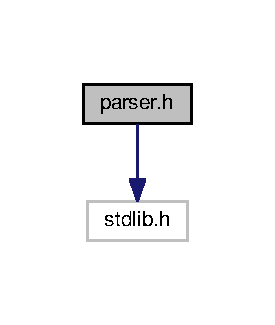
\includegraphics[width=132pt]{parser_8h__incl}
\end{center}
\end{figure}
This graph shows which files directly or indirectly include this file\+:
\nopagebreak
\begin{figure}[H]
\begin{center}
\leavevmode
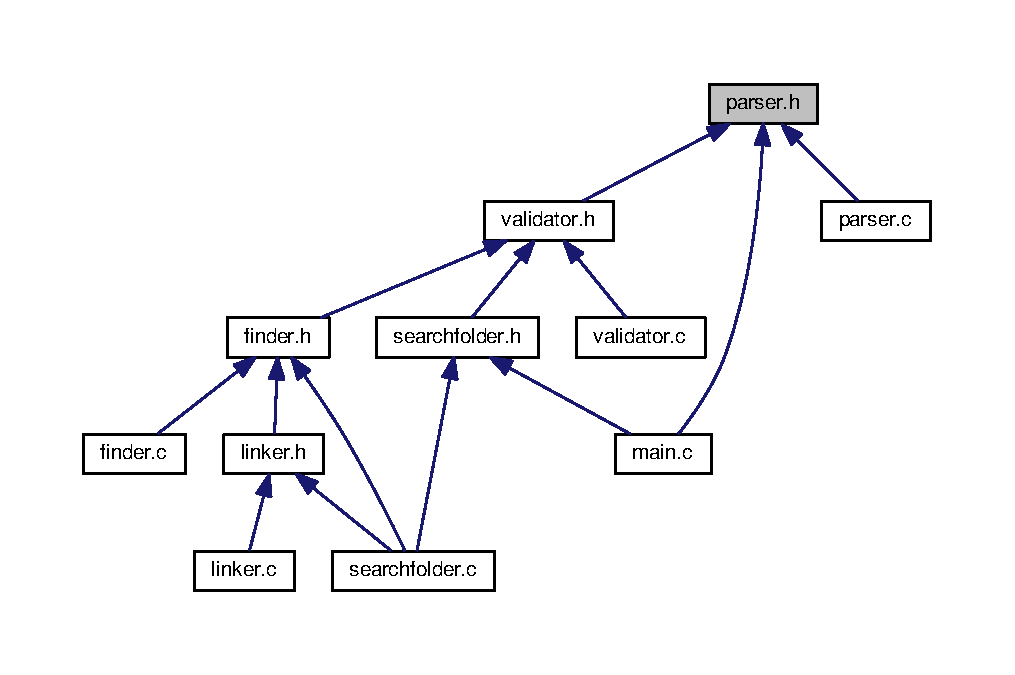
\includegraphics[width=350pt]{parser_8h__dep__incl}
\end{center}
\end{figure}
\subsection*{Data Structures}
\begin{DoxyCompactItemize}
\item 
struct \hyperlink{structparser__t}{parser\+\_\+t}
\begin{DoxyCompactList}\small\item\em Formal expression representation. \end{DoxyCompactList}\end{DoxyCompactItemize}
\subsection*{Typedefs}
\begin{DoxyCompactItemize}
\item 
typedef struct \hyperlink{structparser__t}{parser\+\_\+t} \hyperlink{parser_8h_a402117b92426b41469190a0d4d4397f0}{parser\+\_\+t}
\begin{DoxyCompactList}\small\item\em Formal expression representation. \end{DoxyCompactList}\end{DoxyCompactItemize}
\subsection*{Enumerations}
\begin{DoxyCompactItemize}
\item 
enum \hyperlink{parser_8h_a32088e9f194a33e050822b8c536e03cb}{parser\+\_\+crit\+\_\+type\+\_\+t} \{ {\bfseries O\+P\+E\+R\+A\+T\+OR} = 1 $<$$<$ 7, 
{\bfseries P\+A\+R\+E\+N\+T\+H\+E\+S\+IS} = 1 $<$$<$ 6, 
{\bfseries C\+R\+I\+T\+E\+R\+IA} = 1 $<$$<$ 5
 \}\begin{DoxyCompactList}\small\item\em Type of expression token. \end{DoxyCompactList}
\item 
enum \hyperlink{parser_8h_a4dcbe7148b91f50b0e7f3e08e780861d}{parser\+\_\+crit\+\_\+t} \{ \\*
{\bfseries OR} = O\+P\+E\+R\+A\+T\+OR, 
{\bfseries A\+ND}, 
{\bfseries N\+OT}, 
{\bfseries N\+A\+ME} = C\+R\+I\+T\+E\+R\+IA $\vert$ 3, 
\\*
{\bfseries U\+S\+ER}, 
{\bfseries G\+R\+O\+UP}, 
{\bfseries P\+E\+RM}, 
{\bfseries S\+I\+ZE}, 
\\*
{\bfseries A\+T\+I\+ME}, 
{\bfseries M\+T\+I\+ME}, 
{\bfseries C\+T\+I\+ME}, 
{\bfseries L\+P\+A\+R\+E\+N\+T\+H\+E\+S\+IS} = P\+A\+R\+E\+N\+T\+H\+E\+S\+IS, 
\\*
{\bfseries R\+P\+A\+R\+E\+N\+T\+H\+E\+S\+IS}
 \}\begin{DoxyCompactList}\small\item\em List of possible expression tokens. \end{DoxyCompactList}
\item 
enum \hyperlink{parser_8h_ac721d0db2049edef01e62a2e63ff0472}{parser\+\_\+comp\+\_\+t} \{ {\bfseries M\+AX}, 
{\bfseries M\+IN}, 
{\bfseries E\+X\+A\+CT}
 \}\begin{DoxyCompactList}\small\item\em The comparator used to evaluate criteria values. \end{DoxyCompactList}
\end{DoxyCompactItemize}
\subsection*{Functions}
\begin{DoxyCompactItemize}
\item 
\hyperlink{structparser__t}{parser\+\_\+t} $\ast$ \hyperlink{parser_8h_a570f8d50af35e4863518a619ef74d501}{parser\+\_\+parse} (char $\ast$expression\mbox{[}$\,$\mbox{]}, size\+\_\+t size)
\begin{DoxyCompactList}\small\item\em Parses the string expression, converting it to a {\ttfamily \hyperlink{structparser__t}{parser\+\_\+t}} representation. \end{DoxyCompactList}\item 
void \hyperlink{parser_8h_a680ceeada57c4645e365ba1745d41181}{parser\+\_\+free} (\hyperlink{structparser__t}{parser\+\_\+t} $\ast$expression)
\begin{DoxyCompactList}\small\item\em Frees the memory allocated for a {\ttfamily \hyperlink{structparser__t}{parser\+\_\+t}} instance. \end{DoxyCompactList}\end{DoxyCompactItemize}


\subsection{Detailed Description}
Parses a string expression and return a formal representation. 

Full unit test coverage 

\subsection{Typedef Documentation}
\index{parser.\+h@{parser.\+h}!parser\+\_\+t@{parser\+\_\+t}}
\index{parser\+\_\+t@{parser\+\_\+t}!parser.\+h@{parser.\+h}}
\subsubsection[{\texorpdfstring{parser\+\_\+t}{parser_t}}]{\setlength{\rightskip}{0pt plus 5cm}typedef struct {\bf parser\+\_\+t}  {\bf parser\+\_\+t}}\hypertarget{parser_8h_a402117b92426b41469190a0d4d4397f0}{}\label{parser_8h_a402117b92426b41469190a0d4d4397f0}


Formal expression representation. 

Contains the formal representation of the parsed expression in a ordered chained list. Each instance contains the information about a parsed expression token and the pointer to the {\ttfamily next} parsed expression token.

The order of the tokens in the chained list is not the same as the in the original string representation. Is has been reordered to encoded the priority of the operators and parenthesis in a infix notation 

\subsection{Enumeration Type Documentation}
\index{parser.\+h@{parser.\+h}!parser\+\_\+comp\+\_\+t@{parser\+\_\+comp\+\_\+t}}
\index{parser\+\_\+comp\+\_\+t@{parser\+\_\+comp\+\_\+t}!parser.\+h@{parser.\+h}}
\subsubsection[{\texorpdfstring{parser\+\_\+comp\+\_\+t}{parser_comp_t}}]{\setlength{\rightskip}{0pt plus 5cm}enum {\bf parser\+\_\+comp\+\_\+t}}\hypertarget{parser_8h_ac721d0db2049edef01e62a2e63ff0472}{}\label{parser_8h_ac721d0db2049edef01e62a2e63ff0472}


The comparator used to evaluate criteria values. 

Calculated for criteria that accepts the  in the values.
\begin{DoxyItemize}
\item Example\+: {\ttfamily -\/\+S\+I\+ZE +20k} or {\ttfamily -\/\+N\+A\+ME -\/.\+txt}
\end{DoxyItemize}

\begin{DoxySeeAlso}{See also}
\hyperlink{structparser__t}{parser\+\_\+t} 
\end{DoxySeeAlso}


Definition at line 60 of file parser.\+h.

\index{parser.\+h@{parser.\+h}!parser\+\_\+crit\+\_\+t@{parser\+\_\+crit\+\_\+t}}
\index{parser\+\_\+crit\+\_\+t@{parser\+\_\+crit\+\_\+t}!parser.\+h@{parser.\+h}}
\subsubsection[{\texorpdfstring{parser\+\_\+crit\+\_\+t}{parser_crit_t}}]{\setlength{\rightskip}{0pt plus 5cm}enum {\bf parser\+\_\+crit\+\_\+t}}\hypertarget{parser_8h_a4dcbe7148b91f50b0e7f3e08e780861d}{}\label{parser_8h_a4dcbe7148b91f50b0e7f3e08e780861d}


List of possible expression tokens. 

The enum values encode information\+:
\begin{DoxyItemize}
\item the 3 most significant bits hold the category (operator, criteria or parenthesis)
\item the 4 least significant bits hold the token order
\begin{DoxyItemize}
\item must start at 0 and be consecutive
\end{DoxyItemize}
\item operators are listed by priority A\+SC
\begin{DoxyItemize}
\item the encoded priority information is used in the parsing algorithm
\end{DoxyItemize}
\end{DoxyItemize}

\begin{DoxySeeAlso}{See also}
\hyperlink{parser_8h_a32088e9f194a33e050822b8c536e03cb}{parser\+\_\+crit\+\_\+type\+\_\+t} 

\hyperlink{structparser__t}{parser\+\_\+t} 
\end{DoxySeeAlso}


Definition at line 37 of file parser.\+h.

\index{parser.\+h@{parser.\+h}!parser\+\_\+crit\+\_\+type\+\_\+t@{parser\+\_\+crit\+\_\+type\+\_\+t}}
\index{parser\+\_\+crit\+\_\+type\+\_\+t@{parser\+\_\+crit\+\_\+type\+\_\+t}!parser.\+h@{parser.\+h}}
\subsubsection[{\texorpdfstring{parser\+\_\+crit\+\_\+type\+\_\+t}{parser_crit_type_t}}]{\setlength{\rightskip}{0pt plus 5cm}enum {\bf parser\+\_\+crit\+\_\+type\+\_\+t}}\hypertarget{parser_8h_a32088e9f194a33e050822b8c536e03cb}{}\label{parser_8h_a32088e9f194a33e050822b8c536e03cb}


Type of expression token. 

Used to flag bitwise the {\ttfamily parser\+\_\+crit\+\_\+t} enum values, and later to obtain the category of a given {\ttfamily parser\+\_\+crit\+\_\+t} enum value

\begin{DoxySeeAlso}{See also}
\hyperlink{parser_8h_a4dcbe7148b91f50b0e7f3e08e780861d}{parser\+\_\+crit\+\_\+t} 
\end{DoxySeeAlso}


Definition at line 19 of file parser.\+h.



\subsection{Function Documentation}
\index{parser.\+h@{parser.\+h}!parser\+\_\+free@{parser\+\_\+free}}
\index{parser\+\_\+free@{parser\+\_\+free}!parser.\+h@{parser.\+h}}
\subsubsection[{\texorpdfstring{parser\+\_\+free(parser\+\_\+t $\ast$expression)}{parser_free(parser_t *expression)}}]{\setlength{\rightskip}{0pt plus 5cm}void parser\+\_\+free (
\begin{DoxyParamCaption}
\item[{{\bf parser\+\_\+t} $\ast$}]{expression}
\end{DoxyParamCaption}
)}\hypertarget{parser_8h_a680ceeada57c4645e365ba1745d41181}{}\label{parser_8h_a680ceeada57c4645e365ba1745d41181}


Frees the memory allocated for a {\ttfamily \hyperlink{structparser__t}{parser\+\_\+t}} instance. 

\begin{DoxySeeAlso}{See also}
\hyperlink{structparser__t}{parser\+\_\+t} 
\end{DoxySeeAlso}

\begin{DoxyParams}{Parameters}
{\em expression} & The `parser\+\_\+t instance to free \\
\hline
\end{DoxyParams}


Definition at line 366 of file parser.\+c.

\index{parser.\+h@{parser.\+h}!parser\+\_\+parse@{parser\+\_\+parse}}
\index{parser\+\_\+parse@{parser\+\_\+parse}!parser.\+h@{parser.\+h}}
\subsubsection[{\texorpdfstring{parser\+\_\+parse(char $\ast$expression[], size\+\_\+t size)}{parser_parse(char *expression[], size_t size)}}]{\setlength{\rightskip}{0pt plus 5cm}{\bf parser\+\_\+t}$\ast$ parser\+\_\+parse (
\begin{DoxyParamCaption}
\item[{char $\ast$}]{expression\mbox{[}$\,$\mbox{]}, }
\item[{size\+\_\+t}]{size}
\end{DoxyParamCaption}
)}\hypertarget{parser_8h_a570f8d50af35e4863518a619ef74d501}{}\label{parser_8h_a570f8d50af35e4863518a619ef74d501}


Parses the string expression, converting it to a {\ttfamily \hyperlink{structparser__t}{parser\+\_\+t}} representation. 

This is done in multiple steps\+:
\begin{DoxyEnumerate}
\item tokens syntax is verified
\item criteria values units and comparison characters are verified
\item a object representation is created for each token
\item tokens are reordered to an infix notation encoding the operators priority and parenthesis
\end{DoxyEnumerate}

The algorithm used in step {\itshape 4} is based on the \href{https://en.wikipedia.org/wiki/Shunting-yard_algorithm}{\tt Shunting yard algorithm} (by Edsger Dijkstra). The original algorithm is intended to parse mathematical expressions and was adapt to parse our boolean expressions. \begin{DoxySeeAlso}{See also}
\hyperlink{structparser__t}{parser\+\_\+t}
\end{DoxySeeAlso}

\begin{DoxyParams}{Parameters}
{\em expression} & The list of tokens forming the expression (space splitted) \\
\hline
{\em size} & The number of elements in {\ttfamily expression} \\
\hline
\end{DoxyParams}
\begin{DoxyReturn}{Returns}
A {\ttfamily \hyperlink{structparser__t}{parser\+\_\+t}} representation of the expression, or {\itshape N\+U\+LL} is the expression is invalid 
\end{DoxyReturn}


Definition at line 339 of file parser.\+c.


\hypertarget{validator_8c}{}\section{/home/claudio/git/smart-\/folder/src/validator.c File Reference}
\label{validator_8c}\index{/home/claudio/git/smart-\/folder/src/validator.\+c@{/home/claudio/git/smart-\/folder/src/validator.\+c}}


Critera and operator evaludation functions.  


{\ttfamily \#include $<$string.\+h$>$}\\*
{\ttfamily \#include $<$time.\+h$>$}\\*
{\ttfamily \#include $<$sys/types.\+h$>$}\\*
{\ttfamily \#include \char`\"{}validator.\+h\char`\"{}}\\*
{\ttfamily \#include \char`\"{}logger.\+h\char`\"{}}\\*
Include dependency graph for validator.\+c\+:\nopagebreak
\begin{figure}[H]
\begin{center}
\leavevmode
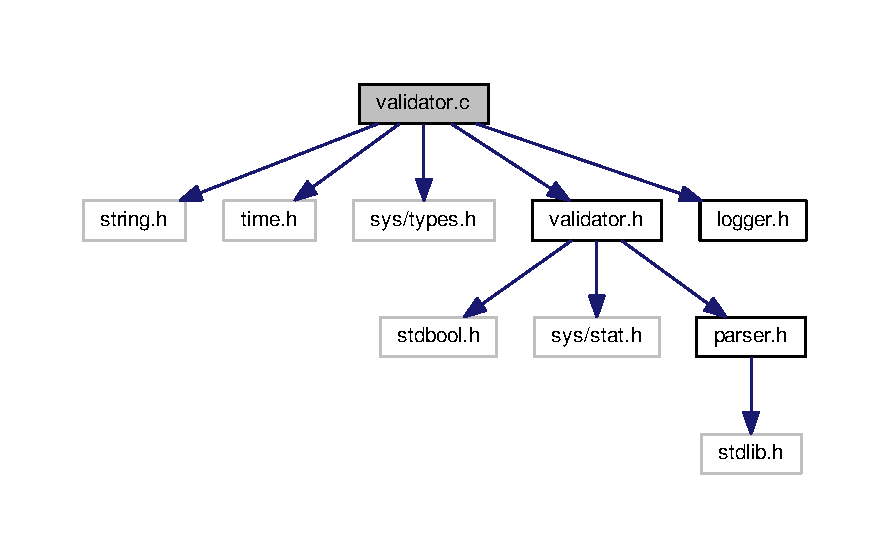
\includegraphics[width=350pt]{validator_8c__incl}
\end{center}
\end{figure}
\subsection*{Macros}
\begin{DoxyCompactItemize}
\item 
\#define \hyperlink{validator_8c_a20f8a4e237e6918372da5e1aec3426c8}{C\+R\+I\+T\+E\+R\+I\+A\+\_\+\+C\+O\+U\+NT}~11\hypertarget{validator_8c_a20f8a4e237e6918372da5e1aec3426c8}{}\label{validator_8c_a20f8a4e237e6918372da5e1aec3426c8}

\begin{DoxyCompactList}\small\item\em Number of criteria/operators. \end{DoxyCompactList}\item 
\#define \hyperlink{validator_8c_abe2627a9935b96daef8d9a2478934647}{P\+E\+R\+M\+\_\+\+O\+P\+T\+I\+O\+N\+S\+\_\+\+C\+O\+U\+NT}~9\hypertarget{validator_8c_abe2627a9935b96daef8d9a2478934647}{}\label{validator_8c_abe2627a9935b96daef8d9a2478934647}

\begin{DoxyCompactList}\small\item\em Number of permission options. \end{DoxyCompactList}\item 
\#define \hyperlink{validator_8c_a77d91bcc6068803c9eff253b1028073e}{C\+R\+I\+T\+E\+R\+I\+A\+\_\+\+O\+R\+D\+E\+R\+\_\+\+M\+A\+SK}~0b1111
\begin{DoxyCompactList}\small\item\em Mask that to apply to {\ttfamily parser\+\_\+crit\+\_\+t} to get criteria index in the enum. \end{DoxyCompactList}\end{DoxyCompactItemize}
\subsection*{Typedefs}
\begin{DoxyCompactItemize}
\item 
typedef bool($\ast$ \hyperlink{validator_8c_ad99afbcae8ae7f7cfee6a97184d5861b}{validate\+\_\+fn\+\_\+t}) (char $\ast$, struct stat $\ast$, \hyperlink{structparser__t}{parser\+\_\+t} $\ast$)\hypertarget{validator_8c_ad99afbcae8ae7f7cfee6a97184d5861b}{}\label{validator_8c_ad99afbcae8ae7f7cfee6a97184d5861b}

\begin{DoxyCompactList}\small\item\em Function pointer for criteria validate functions. \end{DoxyCompactList}\end{DoxyCompactItemize}
\subsection*{Enumerations}
\begin{DoxyCompactItemize}
\item 
enum \hyperlink{validator_8c_a156f9580ff03fe2c43a04418b103e97c}{validate\+\_\+perm\+\_\+type\+\_\+t} \{ {\bfseries R} = 4, 
{\bfseries W} = 2, 
{\bfseries X} = 1
 \}\begin{DoxyCompactList}\small\item\em List of permission types. \end{DoxyCompactList}
\item 
enum \hyperlink{validator_8c_a5de95e832572a2d519fc383840461239}{validate\+\_\+perm\+\_\+owner\+\_\+t} \{ {\bfseries U} = 6, 
{\bfseries G} = 3, 
{\bfseries O} = 0
 \}\begin{DoxyCompactList}\small\item\em List of permission targets. \end{DoxyCompactList}
\end{DoxyCompactItemize}
\subsection*{Functions}
\begin{DoxyCompactItemize}
\item 
static bool \hyperlink{validator_8c_a862284e5fc7d85e05483740c503ef148}{validate\+\_\+exp\+\_\+token} (char $\ast$filename, struct stat $\ast$filestat, \hyperlink{structparser__t}{parser\+\_\+t} $\ast$exp)
\begin{DoxyCompactList}\small\item\em Validates an expression token. \end{DoxyCompactList}\item 
static bool \hyperlink{validator_8c_adaa4bce57cef9baefdf7746d43e0c213}{validate\+\_\+or} (char $\ast$filename, struct stat $\ast$filestat, \hyperlink{structparser__t}{parser\+\_\+t} $\ast$exp)
\begin{DoxyCompactList}\small\item\em Validates OR operators. \end{DoxyCompactList}\item 
static bool \hyperlink{validator_8c_a95a034664a3f37186e065b898fc3d041}{validate\+\_\+and} (char $\ast$filename, struct stat $\ast$filestat, \hyperlink{structparser__t}{parser\+\_\+t} $\ast$exp)
\begin{DoxyCompactList}\small\item\em Validates A\+ND operators. \end{DoxyCompactList}\item 
static bool \hyperlink{validator_8c_a8341e1b958e2ec8cd5d5167212473731}{validate\+\_\+not} (char $\ast$filename, struct stat $\ast$filestat, \hyperlink{structparser__t}{parser\+\_\+t} $\ast$exp)
\begin{DoxyCompactList}\small\item\em Validates N\+OT operators. \end{DoxyCompactList}\item 
static bool \hyperlink{validator_8c_abd410628fdfe4e5df774cc57c13fa88e}{validate\+\_\+name} (char $\ast$filename, struct stat $\ast$filestat, \hyperlink{structparser__t}{parser\+\_\+t} $\ast$exp)
\begin{DoxyCompactList}\small\item\em Validates N\+A\+ME criteria. \end{DoxyCompactList}\item 
static bool \hyperlink{validator_8c_adca99e4146bc36bfb1ea9cd6a1335801}{validate\+\_\+user} (char $\ast$filename, struct stat $\ast$filestat, \hyperlink{structparser__t}{parser\+\_\+t} $\ast$exp)
\begin{DoxyCompactList}\small\item\em Validates U\+S\+ER criteria. \end{DoxyCompactList}\item 
static bool \hyperlink{validator_8c_a372b7bb2456d5211c7dac83eaaa4aec1}{validate\+\_\+group} (char $\ast$filename, struct stat $\ast$filestat, \hyperlink{structparser__t}{parser\+\_\+t} $\ast$exp)
\begin{DoxyCompactList}\small\item\em Validates G\+R\+O\+UP criteria. \end{DoxyCompactList}\item 
static bool \hyperlink{validator_8c_ab8e50ae831fd783fc9d455494d26b905}{validate\+\_\+perm} (char $\ast$filename, struct stat $\ast$filestat, \hyperlink{structparser__t}{parser\+\_\+t} $\ast$exp)
\begin{DoxyCompactList}\small\item\em Validates P\+E\+RM criteria. \end{DoxyCompactList}\item 
static bool \hyperlink{validator_8c_aa410d57420af99c3bdf2e174f3ab3321}{validate\+\_\+size} (char $\ast$filename, struct stat $\ast$filestat, \hyperlink{structparser__t}{parser\+\_\+t} $\ast$exp)
\begin{DoxyCompactList}\small\item\em Validates S\+I\+ZE criteria. \end{DoxyCompactList}\item 
static bool \hyperlink{validator_8c_a09e5b757b61865f2fe4f913e476db459}{validate\+\_\+time} (time\+\_\+t comp\+\_\+time, parser\+\_\+comp\+\_\+t comp, long refseconds)
\begin{DoxyCompactList}\small\item\em Factorizes time related validation. \end{DoxyCompactList}\item 
static bool \hyperlink{validator_8c_a8ca6f2c0ab321df18548c3e12c87b703}{validate\+\_\+atime} (char $\ast$filename, struct stat $\ast$filestat, \hyperlink{structparser__t}{parser\+\_\+t} $\ast$exp)
\begin{DoxyCompactList}\small\item\em Validates A\+T\+I\+ME criteria. \end{DoxyCompactList}\item 
static bool \hyperlink{validator_8c_aee84fd5cf26129acf79e7dfd2a5185c1}{validate\+\_\+mtime} (char $\ast$filename, struct stat $\ast$filestat, \hyperlink{structparser__t}{parser\+\_\+t} $\ast$exp)
\begin{DoxyCompactList}\small\item\em Validates M\+T\+I\+ME criteria. \end{DoxyCompactList}\item 
static bool \hyperlink{validator_8c_aa717edec98675daa659c16a1e51d2fc0}{validate\+\_\+ctime} (char $\ast$filename, struct stat $\ast$filestat, \hyperlink{structparser__t}{parser\+\_\+t} $\ast$exp)
\begin{DoxyCompactList}\small\item\em Validates C\+T\+I\+ME criteria. \end{DoxyCompactList}\item 
bool \hyperlink{validator_8c_aa0281da3748596d0f34db26d16661771}{validator\+\_\+validate} (char $\ast$filename, struct stat $\ast$filestat, \hyperlink{structparser__t}{parser\+\_\+t} $\ast$exp)
\begin{DoxyCompactList}\small\item\em Validates a file against an expression. \end{DoxyCompactList}\end{DoxyCompactItemize}
\subsection*{Variables}
\begin{DoxyCompactItemize}
\item 
static int \hyperlink{validator_8c_a59a13bfa9a783bc3c4d64cc8671db7ba}{P\+E\+R\+M\+\_\+\+O\+P\+T\+I\+O\+NS} \mbox{[}\hyperlink{validator_8c_abe2627a9935b96daef8d9a2478934647}{P\+E\+R\+M\+\_\+\+O\+P\+T\+I\+O\+N\+S\+\_\+\+C\+O\+U\+NT}\mbox{]} = \{R $<$$<$ U, W $<$$<$ U, X $<$$<$ U, R $<$$<$ G, W $<$$<$ G, X $<$$<$ G, R $<$$<$ O, W $<$$<$ O, X $<$$<$ O\}
\begin{DoxyCompactList}\small\item\em List of all permission options. \end{DoxyCompactList}\item 
static int \hyperlink{validator_8c_a119982f507a1f4dbe52025a97a127f9f}{P\+E\+R\+M\+\_\+\+F\+L\+A\+GS} \mbox{[}\hyperlink{validator_8c_abe2627a9935b96daef8d9a2478934647}{P\+E\+R\+M\+\_\+\+O\+P\+T\+I\+O\+N\+S\+\_\+\+C\+O\+U\+NT}\mbox{]}
\begin{DoxyCompactList}\small\item\em List of all \href{http://pubs.opengroup.org/onlinepubs/7908799/xsh/sysstat.h.html}{\tt OS permission flags} matching the permission options. \end{DoxyCompactList}\item 
static \hyperlink{validator_8c_ad99afbcae8ae7f7cfee6a97184d5861b}{validate\+\_\+fn\+\_\+t} \hyperlink{validator_8c_a9839e177025c582f4ad9d7c007141636}{validators} \mbox{[}\hyperlink{validator_8c_a20f8a4e237e6918372da5e1aec3426c8}{C\+R\+I\+T\+E\+R\+I\+A\+\_\+\+C\+O\+U\+NT}\mbox{]}
\begin{DoxyCompactList}\small\item\em List of of criteria validate functions. \end{DoxyCompactList}\end{DoxyCompactItemize}


\subsection{Detailed Description}
Critera and operator evaludation functions. 

Contains the logic to evaluate each possible critera and operator. 

\subsection{Macro Definition Documentation}
\index{validator.\+c@{validator.\+c}!C\+R\+I\+T\+E\+R\+I\+A\+\_\+\+O\+R\+D\+E\+R\+\_\+\+M\+A\+SK@{C\+R\+I\+T\+E\+R\+I\+A\+\_\+\+O\+R\+D\+E\+R\+\_\+\+M\+A\+SK}}
\index{C\+R\+I\+T\+E\+R\+I\+A\+\_\+\+O\+R\+D\+E\+R\+\_\+\+M\+A\+SK@{C\+R\+I\+T\+E\+R\+I\+A\+\_\+\+O\+R\+D\+E\+R\+\_\+\+M\+A\+SK}!validator.\+c@{validator.\+c}}
\subsubsection[{\texorpdfstring{C\+R\+I\+T\+E\+R\+I\+A\+\_\+\+O\+R\+D\+E\+R\+\_\+\+M\+A\+SK}{CRITERIA_ORDER_MASK}}]{\setlength{\rightskip}{0pt plus 5cm}\#define C\+R\+I\+T\+E\+R\+I\+A\+\_\+\+O\+R\+D\+E\+R\+\_\+\+M\+A\+SK~0b1111}\hypertarget{validator_8c_a77d91bcc6068803c9eff253b1028073e}{}\label{validator_8c_a77d91bcc6068803c9eff253b1028073e}


Mask that to apply to {\ttfamily parser\+\_\+crit\+\_\+t} to get criteria index in the enum. 

\begin{DoxySeeAlso}{See also}
parser\+\_\+crit\+\_\+t 
\end{DoxySeeAlso}


Definition at line 18 of file validator.\+c.



\subsection{Enumeration Type Documentation}
\index{validator.\+c@{validator.\+c}!validate\+\_\+perm\+\_\+owner\+\_\+t@{validate\+\_\+perm\+\_\+owner\+\_\+t}}
\index{validate\+\_\+perm\+\_\+owner\+\_\+t@{validate\+\_\+perm\+\_\+owner\+\_\+t}!validator.\+c@{validator.\+c}}
\subsubsection[{\texorpdfstring{validate\+\_\+perm\+\_\+owner\+\_\+t}{validate_perm_owner_t}}]{\setlength{\rightskip}{0pt plus 5cm}enum {\bf validate\+\_\+perm\+\_\+owner\+\_\+t}}\hypertarget{validator_8c_a5de95e832572a2d519fc383840461239}{}\label{validator_8c_a5de95e832572a2d519fc383840461239}


List of permission targets. 


\begin{DoxyItemize}
\item user
\item group
\item owner
\end{DoxyItemize}

Used to shift {\ttfamily validate\+\_\+perm\+\_\+type\+\_\+t} bitwise \begin{DoxySeeAlso}{See also}
\hyperlink{validator_8c_a156f9580ff03fe2c43a04418b103e97c}{validate\+\_\+perm\+\_\+type\+\_\+t} 
\end{DoxySeeAlso}


Definition at line 41 of file validator.\+c.

\index{validator.\+c@{validator.\+c}!validate\+\_\+perm\+\_\+type\+\_\+t@{validate\+\_\+perm\+\_\+type\+\_\+t}}
\index{validate\+\_\+perm\+\_\+type\+\_\+t@{validate\+\_\+perm\+\_\+type\+\_\+t}!validator.\+c@{validator.\+c}}
\subsubsection[{\texorpdfstring{validate\+\_\+perm\+\_\+type\+\_\+t}{validate_perm_type_t}}]{\setlength{\rightskip}{0pt plus 5cm}enum {\bf validate\+\_\+perm\+\_\+type\+\_\+t}}\hypertarget{validator_8c_a156f9580ff03fe2c43a04418b103e97c}{}\label{validator_8c_a156f9580ff03fe2c43a04418b103e97c}


List of permission types. 


\begin{DoxyItemize}
\item read
\item write
\item execute
\end{DoxyItemize}

\begin{DoxySeeAlso}{See also}
\hyperlink{validator_8c_a5de95e832572a2d519fc383840461239}{validate\+\_\+perm\+\_\+owner\+\_\+t} 
\end{DoxySeeAlso}


Definition at line 27 of file validator.\+c.



\subsection{Function Documentation}
\index{validator.\+c@{validator.\+c}!validate\+\_\+and@{validate\+\_\+and}}
\index{validate\+\_\+and@{validate\+\_\+and}!validator.\+c@{validator.\+c}}
\subsubsection[{\texorpdfstring{validate\+\_\+and(char $\ast$filename, struct stat $\ast$filestat, parser\+\_\+t $\ast$exp)}{validate_and(char *filename, struct stat *filestat, parser_t *exp)}}]{\setlength{\rightskip}{0pt plus 5cm}static bool validate\+\_\+and (
\begin{DoxyParamCaption}
\item[{char $\ast$}]{filename, }
\item[{struct stat $\ast$}]{filestat, }
\item[{{\bf parser\+\_\+t} $\ast$}]{exp}
\end{DoxyParamCaption}
)\hspace{0.3cm}{\ttfamily [static]}}\hypertarget{validator_8c_a95a034664a3f37186e065b898fc3d041}{}\label{validator_8c_a95a034664a3f37186e065b898fc3d041}


Validates A\+ND operators. 



Definition at line 72 of file validator.\+c.

\index{validator.\+c@{validator.\+c}!validate\+\_\+atime@{validate\+\_\+atime}}
\index{validate\+\_\+atime@{validate\+\_\+atime}!validator.\+c@{validator.\+c}}
\subsubsection[{\texorpdfstring{validate\+\_\+atime(char $\ast$filename, struct stat $\ast$filestat, parser\+\_\+t $\ast$exp)}{validate_atime(char *filename, struct stat *filestat, parser_t *exp)}}]{\setlength{\rightskip}{0pt plus 5cm}static bool validate\+\_\+atime (
\begin{DoxyParamCaption}
\item[{char $\ast$}]{filename, }
\item[{struct stat $\ast$}]{filestat, }
\item[{{\bf parser\+\_\+t} $\ast$}]{exp}
\end{DoxyParamCaption}
)\hspace{0.3cm}{\ttfamily [static]}}\hypertarget{validator_8c_a8ca6f2c0ab321df18548c3e12c87b703}{}\label{validator_8c_a8ca6f2c0ab321df18548c3e12c87b703}


Validates A\+T\+I\+ME criteria. 



Definition at line 131 of file validator.\+c.

\index{validator.\+c@{validator.\+c}!validate\+\_\+ctime@{validate\+\_\+ctime}}
\index{validate\+\_\+ctime@{validate\+\_\+ctime}!validator.\+c@{validator.\+c}}
\subsubsection[{\texorpdfstring{validate\+\_\+ctime(char $\ast$filename, struct stat $\ast$filestat, parser\+\_\+t $\ast$exp)}{validate_ctime(char *filename, struct stat *filestat, parser_t *exp)}}]{\setlength{\rightskip}{0pt plus 5cm}static bool validate\+\_\+ctime (
\begin{DoxyParamCaption}
\item[{char $\ast$}]{filename, }
\item[{struct stat $\ast$}]{filestat, }
\item[{{\bf parser\+\_\+t} $\ast$}]{exp}
\end{DoxyParamCaption}
)\hspace{0.3cm}{\ttfamily [static]}}\hypertarget{validator_8c_aa717edec98675daa659c16a1e51d2fc0}{}\label{validator_8c_aa717edec98675daa659c16a1e51d2fc0}


Validates C\+T\+I\+ME criteria. 



Definition at line 143 of file validator.\+c.

\index{validator.\+c@{validator.\+c}!validate\+\_\+exp\+\_\+token@{validate\+\_\+exp\+\_\+token}}
\index{validate\+\_\+exp\+\_\+token@{validate\+\_\+exp\+\_\+token}!validator.\+c@{validator.\+c}}
\subsubsection[{\texorpdfstring{validate\+\_\+exp\+\_\+token(char $\ast$filename, struct stat $\ast$filestat, parser\+\_\+t $\ast$exp)}{validate_exp_token(char *filename, struct stat *filestat, parser_t *exp)}}]{\setlength{\rightskip}{0pt plus 5cm}static bool validate\+\_\+exp\+\_\+token (
\begin{DoxyParamCaption}
\item[{char $\ast$}]{filename, }
\item[{struct stat $\ast$}]{filestat, }
\item[{{\bf parser\+\_\+t} $\ast$}]{exp}
\end{DoxyParamCaption}
)\hspace{0.3cm}{\ttfamily [static]}}\hypertarget{validator_8c_a862284e5fc7d85e05483740c503ef148}{}\label{validator_8c_a862284e5fc7d85e05483740c503ef148}


Validates an expression token. 

Retrieves the validate function corrsponding to the expression token, which can be a criteria or an operator 

Definition at line 169 of file validator.\+c.

\index{validator.\+c@{validator.\+c}!validate\+\_\+group@{validate\+\_\+group}}
\index{validate\+\_\+group@{validate\+\_\+group}!validator.\+c@{validator.\+c}}
\subsubsection[{\texorpdfstring{validate\+\_\+group(char $\ast$filename, struct stat $\ast$filestat, parser\+\_\+t $\ast$exp)}{validate_group(char *filename, struct stat *filestat, parser_t *exp)}}]{\setlength{\rightskip}{0pt plus 5cm}static bool validate\+\_\+group (
\begin{DoxyParamCaption}
\item[{char $\ast$}]{filename, }
\item[{struct stat $\ast$}]{filestat, }
\item[{{\bf parser\+\_\+t} $\ast$}]{exp}
\end{DoxyParamCaption}
)\hspace{0.3cm}{\ttfamily [static]}}\hypertarget{validator_8c_a372b7bb2456d5211c7dac83eaaa4aec1}{}\label{validator_8c_a372b7bb2456d5211c7dac83eaaa4aec1}


Validates G\+R\+O\+UP criteria. 



Definition at line 96 of file validator.\+c.

\index{validator.\+c@{validator.\+c}!validate\+\_\+mtime@{validate\+\_\+mtime}}
\index{validate\+\_\+mtime@{validate\+\_\+mtime}!validator.\+c@{validator.\+c}}
\subsubsection[{\texorpdfstring{validate\+\_\+mtime(char $\ast$filename, struct stat $\ast$filestat, parser\+\_\+t $\ast$exp)}{validate_mtime(char *filename, struct stat *filestat, parser_t *exp)}}]{\setlength{\rightskip}{0pt plus 5cm}static bool validate\+\_\+mtime (
\begin{DoxyParamCaption}
\item[{char $\ast$}]{filename, }
\item[{struct stat $\ast$}]{filestat, }
\item[{{\bf parser\+\_\+t} $\ast$}]{exp}
\end{DoxyParamCaption}
)\hspace{0.3cm}{\ttfamily [static]}}\hypertarget{validator_8c_aee84fd5cf26129acf79e7dfd2a5185c1}{}\label{validator_8c_aee84fd5cf26129acf79e7dfd2a5185c1}


Validates M\+T\+I\+ME criteria. 



Definition at line 137 of file validator.\+c.

\index{validator.\+c@{validator.\+c}!validate\+\_\+name@{validate\+\_\+name}}
\index{validate\+\_\+name@{validate\+\_\+name}!validator.\+c@{validator.\+c}}
\subsubsection[{\texorpdfstring{validate\+\_\+name(char $\ast$filename, struct stat $\ast$filestat, parser\+\_\+t $\ast$exp)}{validate_name(char *filename, struct stat *filestat, parser_t *exp)}}]{\setlength{\rightskip}{0pt plus 5cm}static bool validate\+\_\+name (
\begin{DoxyParamCaption}
\item[{char $\ast$}]{filename, }
\item[{struct stat $\ast$}]{filestat, }
\item[{{\bf parser\+\_\+t} $\ast$}]{exp}
\end{DoxyParamCaption}
)\hspace{0.3cm}{\ttfamily [static]}}\hypertarget{validator_8c_abd410628fdfe4e5df774cc57c13fa88e}{}\label{validator_8c_abd410628fdfe4e5df774cc57c13fa88e}


Validates N\+A\+ME criteria. 



Definition at line 83 of file validator.\+c.

\index{validator.\+c@{validator.\+c}!validate\+\_\+not@{validate\+\_\+not}}
\index{validate\+\_\+not@{validate\+\_\+not}!validator.\+c@{validator.\+c}}
\subsubsection[{\texorpdfstring{validate\+\_\+not(char $\ast$filename, struct stat $\ast$filestat, parser\+\_\+t $\ast$exp)}{validate_not(char *filename, struct stat *filestat, parser_t *exp)}}]{\setlength{\rightskip}{0pt plus 5cm}static bool validate\+\_\+not (
\begin{DoxyParamCaption}
\item[{char $\ast$}]{filename, }
\item[{struct stat $\ast$}]{filestat, }
\item[{{\bf parser\+\_\+t} $\ast$}]{exp}
\end{DoxyParamCaption}
)\hspace{0.3cm}{\ttfamily [static]}}\hypertarget{validator_8c_a8341e1b958e2ec8cd5d5167212473731}{}\label{validator_8c_a8341e1b958e2ec8cd5d5167212473731}


Validates N\+OT operators. 



Definition at line 78 of file validator.\+c.

\index{validator.\+c@{validator.\+c}!validate\+\_\+or@{validate\+\_\+or}}
\index{validate\+\_\+or@{validate\+\_\+or}!validator.\+c@{validator.\+c}}
\subsubsection[{\texorpdfstring{validate\+\_\+or(char $\ast$filename, struct stat $\ast$filestat, parser\+\_\+t $\ast$exp)}{validate_or(char *filename, struct stat *filestat, parser_t *exp)}}]{\setlength{\rightskip}{0pt plus 5cm}static bool validate\+\_\+or (
\begin{DoxyParamCaption}
\item[{char $\ast$}]{filename, }
\item[{struct stat $\ast$}]{filestat, }
\item[{{\bf parser\+\_\+t} $\ast$}]{exp}
\end{DoxyParamCaption}
)\hspace{0.3cm}{\ttfamily [static]}}\hypertarget{validator_8c_adaa4bce57cef9baefdf7746d43e0c213}{}\label{validator_8c_adaa4bce57cef9baefdf7746d43e0c213}


Validates OR operators. 



Definition at line 66 of file validator.\+c.

\index{validator.\+c@{validator.\+c}!validate\+\_\+perm@{validate\+\_\+perm}}
\index{validate\+\_\+perm@{validate\+\_\+perm}!validator.\+c@{validator.\+c}}
\subsubsection[{\texorpdfstring{validate\+\_\+perm(char $\ast$filename, struct stat $\ast$filestat, parser\+\_\+t $\ast$exp)}{validate_perm(char *filename, struct stat *filestat, parser_t *exp)}}]{\setlength{\rightskip}{0pt plus 5cm}static bool validate\+\_\+perm (
\begin{DoxyParamCaption}
\item[{char $\ast$}]{filename, }
\item[{struct stat $\ast$}]{filestat, }
\item[{{\bf parser\+\_\+t} $\ast$}]{exp}
\end{DoxyParamCaption}
)\hspace{0.3cm}{\ttfamily [static]}}\hypertarget{validator_8c_ab8e50ae831fd783fc9d455494d26b905}{}\label{validator_8c_ab8e50ae831fd783fc9d455494d26b905}


Validates P\+E\+RM criteria. 



Definition at line 102 of file validator.\+c.

\index{validator.\+c@{validator.\+c}!validate\+\_\+size@{validate\+\_\+size}}
\index{validate\+\_\+size@{validate\+\_\+size}!validator.\+c@{validator.\+c}}
\subsubsection[{\texorpdfstring{validate\+\_\+size(char $\ast$filename, struct stat $\ast$filestat, parser\+\_\+t $\ast$exp)}{validate_size(char *filename, struct stat *filestat, parser_t *exp)}}]{\setlength{\rightskip}{0pt plus 5cm}static bool validate\+\_\+size (
\begin{DoxyParamCaption}
\item[{char $\ast$}]{filename, }
\item[{struct stat $\ast$}]{filestat, }
\item[{{\bf parser\+\_\+t} $\ast$}]{exp}
\end{DoxyParamCaption}
)\hspace{0.3cm}{\ttfamily [static]}}\hypertarget{validator_8c_aa410d57420af99c3bdf2e174f3ab3321}{}\label{validator_8c_aa410d57420af99c3bdf2e174f3ab3321}


Validates S\+I\+ZE criteria. 



Definition at line 117 of file validator.\+c.

\index{validator.\+c@{validator.\+c}!validate\+\_\+time@{validate\+\_\+time}}
\index{validate\+\_\+time@{validate\+\_\+time}!validator.\+c@{validator.\+c}}
\subsubsection[{\texorpdfstring{validate\+\_\+time(time\+\_\+t comp\+\_\+time, parser\+\_\+comp\+\_\+t comp, long refseconds)}{validate_time(time_t comp_time, parser_comp_t comp, long refseconds)}}]{\setlength{\rightskip}{0pt plus 5cm}static bool validate\+\_\+time (
\begin{DoxyParamCaption}
\item[{time\+\_\+t}]{comp\+\_\+time, }
\item[{parser\+\_\+comp\+\_\+t}]{comp, }
\item[{long}]{refseconds}
\end{DoxyParamCaption}
)\hspace{0.3cm}{\ttfamily [static]}}\hypertarget{validator_8c_a09e5b757b61865f2fe4f913e476db459}{}\label{validator_8c_a09e5b757b61865f2fe4f913e476db459}


Factorizes time related validation. 



Definition at line 124 of file validator.\+c.

\index{validator.\+c@{validator.\+c}!validate\+\_\+user@{validate\+\_\+user}}
\index{validate\+\_\+user@{validate\+\_\+user}!validator.\+c@{validator.\+c}}
\subsubsection[{\texorpdfstring{validate\+\_\+user(char $\ast$filename, struct stat $\ast$filestat, parser\+\_\+t $\ast$exp)}{validate_user(char *filename, struct stat *filestat, parser_t *exp)}}]{\setlength{\rightskip}{0pt plus 5cm}static bool validate\+\_\+user (
\begin{DoxyParamCaption}
\item[{char $\ast$}]{filename, }
\item[{struct stat $\ast$}]{filestat, }
\item[{{\bf parser\+\_\+t} $\ast$}]{exp}
\end{DoxyParamCaption}
)\hspace{0.3cm}{\ttfamily [static]}}\hypertarget{validator_8c_adca99e4146bc36bfb1ea9cd6a1335801}{}\label{validator_8c_adca99e4146bc36bfb1ea9cd6a1335801}


Validates U\+S\+ER criteria. 



Definition at line 90 of file validator.\+c.

\index{validator.\+c@{validator.\+c}!validator\+\_\+validate@{validator\+\_\+validate}}
\index{validator\+\_\+validate@{validator\+\_\+validate}!validator.\+c@{validator.\+c}}
\subsubsection[{\texorpdfstring{validator\+\_\+validate(char $\ast$filename, struct stat $\ast$filestat, parser\+\_\+t $\ast$exp)}{validator_validate(char *filename, struct stat *filestat, parser_t *exp)}}]{\setlength{\rightskip}{0pt plus 5cm}bool validator\+\_\+validate (
\begin{DoxyParamCaption}
\item[{char $\ast$}]{filename, }
\item[{struct stat $\ast$}]{filestat, }
\item[{{\bf parser\+\_\+t} $\ast$}]{exp}
\end{DoxyParamCaption}
)}\hypertarget{validator_8c_aa0281da3748596d0f34db26d16661771}{}\label{validator_8c_aa0281da3748596d0f34db26d16661771}


Validates a file against an expression. 



Definition at line 179 of file validator.\+c.



\subsection{Variable Documentation}
\index{validator.\+c@{validator.\+c}!P\+E\+R\+M\+\_\+\+F\+L\+A\+GS@{P\+E\+R\+M\+\_\+\+F\+L\+A\+GS}}
\index{P\+E\+R\+M\+\_\+\+F\+L\+A\+GS@{P\+E\+R\+M\+\_\+\+F\+L\+A\+GS}!validator.\+c@{validator.\+c}}
\subsubsection[{\texorpdfstring{P\+E\+R\+M\+\_\+\+F\+L\+A\+GS}{PERM_FLAGS}}]{\setlength{\rightskip}{0pt plus 5cm}int P\+E\+R\+M\+\_\+\+F\+L\+A\+GS\mbox{[}{\bf P\+E\+R\+M\+\_\+\+O\+P\+T\+I\+O\+N\+S\+\_\+\+C\+O\+U\+NT}\mbox{]}\hspace{0.3cm}{\ttfamily [static]}}\hypertarget{validator_8c_a119982f507a1f4dbe52025a97a127f9f}{}\label{validator_8c_a119982f507a1f4dbe52025a97a127f9f}
{\bfseries Initial value\+:}
\begin{DoxyCode}
= \{S\_IRUSR, S\_IWUSR, S\_IXUSR, S\_IRGRP, S\_IWGRP,
                                             S\_IXGRP, S\_IROTH, S\_IWOTH, S\_IXOTH\}
\end{DoxyCode}


List of all \href{http://pubs.opengroup.org/onlinepubs/7908799/xsh/sysstat.h.html}{\tt OS permission flags} matching the permission options. 

\begin{DoxySeeAlso}{See also}
\hyperlink{validator_8c_a156f9580ff03fe2c43a04418b103e97c}{validate\+\_\+perm\+\_\+type\+\_\+t} 

\hyperlink{validator_8c_a59a13bfa9a783bc3c4d64cc8671db7ba}{P\+E\+R\+M\+\_\+\+O\+P\+T\+I\+O\+NS} 
\end{DoxySeeAlso}


Definition at line 60 of file validator.\+c.

\index{validator.\+c@{validator.\+c}!P\+E\+R\+M\+\_\+\+O\+P\+T\+I\+O\+NS@{P\+E\+R\+M\+\_\+\+O\+P\+T\+I\+O\+NS}}
\index{P\+E\+R\+M\+\_\+\+O\+P\+T\+I\+O\+NS@{P\+E\+R\+M\+\_\+\+O\+P\+T\+I\+O\+NS}!validator.\+c@{validator.\+c}}
\subsubsection[{\texorpdfstring{P\+E\+R\+M\+\_\+\+O\+P\+T\+I\+O\+NS}{PERM_OPTIONS}}]{\setlength{\rightskip}{0pt plus 5cm}int P\+E\+R\+M\+\_\+\+O\+P\+T\+I\+O\+NS\mbox{[}{\bf P\+E\+R\+M\+\_\+\+O\+P\+T\+I\+O\+N\+S\+\_\+\+C\+O\+U\+NT}\mbox{]} = \{R $<$$<$ U, W $<$$<$ U, X $<$$<$ U, R $<$$<$ G, W $<$$<$ G, X $<$$<$ G, R $<$$<$ O, W $<$$<$ O, X $<$$<$ O\}\hspace{0.3cm}{\ttfamily [static]}}\hypertarget{validator_8c_a59a13bfa9a783bc3c4d64cc8671db7ba}{}\label{validator_8c_a59a13bfa9a783bc3c4d64cc8671db7ba}


List of all permission options. 

Composed by combining {\ttfamily validate\+\_\+perm\+\_\+type\+\_\+t} and {\ttfamily validate\+\_\+perm\+\_\+owner\+\_\+t} \begin{DoxySeeAlso}{See also}
\hyperlink{validator_8c_a156f9580ff03fe2c43a04418b103e97c}{validate\+\_\+perm\+\_\+type\+\_\+t} 

\hyperlink{validator_8c_a5de95e832572a2d519fc383840461239}{validate\+\_\+perm\+\_\+owner\+\_\+t} 
\end{DoxySeeAlso}


Definition at line 53 of file validator.\+c.

\index{validator.\+c@{validator.\+c}!validators@{validators}}
\index{validators@{validators}!validator.\+c@{validator.\+c}}
\subsubsection[{\texorpdfstring{validators}{validators}}]{\setlength{\rightskip}{0pt plus 5cm}{\bf validate\+\_\+fn\+\_\+t} validators\mbox{[}{\bf C\+R\+I\+T\+E\+R\+I\+A\+\_\+\+C\+O\+U\+NT}\mbox{]}\hspace{0.3cm}{\ttfamily [static]}}\hypertarget{validator_8c_a9839e177025c582f4ad9d7c007141636}{}\label{validator_8c_a9839e177025c582f4ad9d7c007141636}
{\bfseries Initial value\+:}
\begin{DoxyCode}
= \{&\hyperlink{validator_8c_adaa4bce57cef9baefdf7746d43e0c213}{validate\_or},    &\hyperlink{validator_8c_a95a034664a3f37186e065b898fc3d041}{validate\_and},   &\hyperlink{validator_8c_a8341e1b958e2ec8cd5d5167212473731}{validate\_not},  &
      \hyperlink{validator_8c_abd410628fdfe4e5df774cc57c13fa88e}{validate\_name},
                                                   &\hyperlink{validator_8c_adca99e4146bc36bfb1ea9cd6a1335801}{validate\_user},  &
      \hyperlink{validator_8c_a372b7bb2456d5211c7dac83eaaa4aec1}{validate\_group}, &\hyperlink{validator_8c_ab8e50ae831fd783fc9d455494d26b905}{validate\_perm}, &\hyperlink{validator_8c_aa410d57420af99c3bdf2e174f3ab3321}{validate\_size},
                                                   &\hyperlink{validator_8c_a8ca6f2c0ab321df18548c3e12c87b703}{validate\_atime}, &
      \hyperlink{validator_8c_aee84fd5cf26129acf79e7dfd2a5185c1}{validate\_mtime}, &\hyperlink{validator_8c_aa717edec98675daa659c16a1e51d2fc0}{validate\_ctime}\}
\end{DoxyCode}


List of of criteria validate functions. 

Array contained the list of all the criteria specific validate functions The order is important as it must match the index of the criteria in {\ttfamily parser\+\_\+crit\+\_\+t}

\begin{DoxySeeAlso}{See also}
parser\+\_\+crit\+\_\+t 

\hyperlink{validator_8c_ad99afbcae8ae7f7cfee6a97184d5861b}{validate\+\_\+fn\+\_\+t} 

\hyperlink{validator_8c_a77d91bcc6068803c9eff253b1028073e}{C\+R\+I\+T\+E\+R\+I\+A\+\_\+\+O\+R\+D\+E\+R\+\_\+\+M\+A\+SK} 
\end{DoxySeeAlso}


Definition at line 160 of file validator.\+c.


\hypertarget{validator_8h}{}\section{validator.\+h File Reference}
\label{validator_8h}\index{validator.\+h@{validator.\+h}}


Validates files against a parsed criteria expression.  


{\ttfamily \#include $<$stdbool.\+h$>$}\\*
{\ttfamily \#include $<$sys/stat.\+h$>$}\\*
{\ttfamily \#include \char`\"{}parser.\+h\char`\"{}}\\*
Include dependency graph for validator.\+h\+:\nopagebreak
\begin{figure}[H]
\begin{center}
\leavevmode
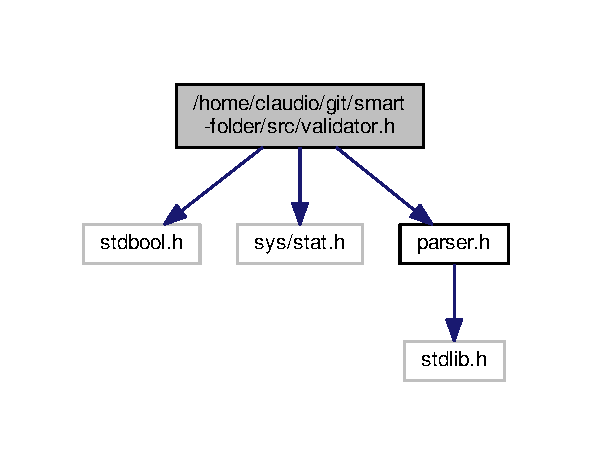
\includegraphics[width=284pt]{validator_8h__incl}
\end{center}
\end{figure}
This graph shows which files directly or indirectly include this file\+:
\nopagebreak
\begin{figure}[H]
\begin{center}
\leavevmode
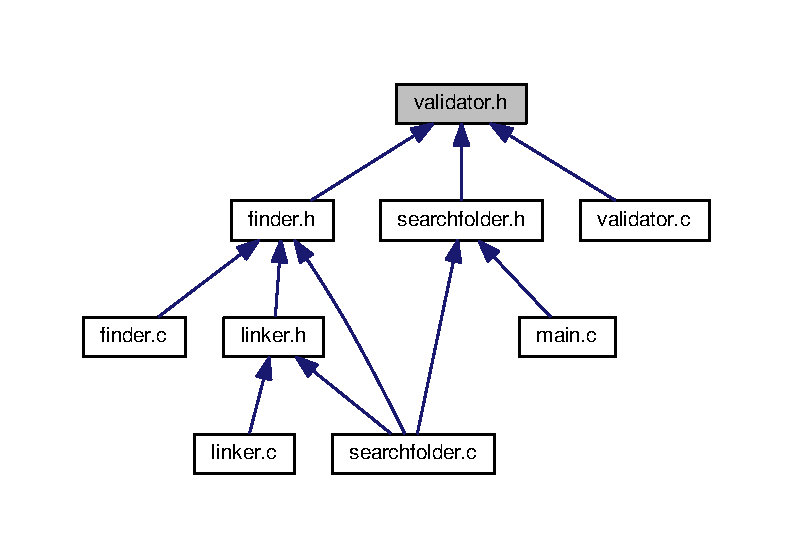
\includegraphics[width=350pt]{validator_8h__dep__incl}
\end{center}
\end{figure}
\subsection*{Functions}
\begin{DoxyCompactItemize}
\item 
bool \hyperlink{validator_8h_a0abc93342b9898145ea067c4a538022a}{validator\+\_\+validate} (char $\ast$filename, struct stat $\ast$filestat, \hyperlink{structparser__t}{parser\+\_\+t} $\ast$expression)
\begin{DoxyCompactList}\small\item\em Validates a file against an expression. \end{DoxyCompactList}\end{DoxyCompactItemize}


\subsection{Detailed Description}
Validates files against a parsed criteria expression. 



\subsection{Function Documentation}
\index{validator.\+h@{validator.\+h}!validator\+\_\+validate@{validator\+\_\+validate}}
\index{validator\+\_\+validate@{validator\+\_\+validate}!validator.\+h@{validator.\+h}}
\subsubsection[{\texorpdfstring{validator\+\_\+validate(char $\ast$filename, struct stat $\ast$filestat, parser\+\_\+t $\ast$expression)}{validator_validate(char *filename, struct stat *filestat, parser_t *expression)}}]{\setlength{\rightskip}{0pt plus 5cm}bool validator\+\_\+validate (
\begin{DoxyParamCaption}
\item[{char $\ast$}]{filename, }
\item[{struct stat $\ast$}]{filestat, }
\item[{{\bf parser\+\_\+t} $\ast$}]{exp}
\end{DoxyParamCaption}
)}\hypertarget{validator_8h_a0abc93342b9898145ea067c4a538022a}{}\label{validator_8h_a0abc93342b9898145ea067c4a538022a}


Validates a file against an expression. 


\begin{DoxyParams}{Parameters}
{\em filename} & The file\textquotesingle{}s name \\
\hline
{\em filestat} & The file\textquotesingle{}s attributes \\
\hline
{\em expression} & The expression used to validate the file \\
\hline
\end{DoxyParams}
\begin{DoxyReturn}{Returns}
If the file is valid
\end{DoxyReturn}


Definition at line 179 of file validator.\+c.


%--- End generated contents ---

% Index
\backmatter
\newpage
\phantomsection
\clearemptydoublepage
\addcontentsline{toc}{chapter}{Index}
\printindex

\end{document}
